%
%DIF LATEXDIFF DIFFERENCE FILE
%DIF DEL report-slides_old.tex   Sat Aug 13 02:40:26 2022
%DIF ADD report-slides_new.tex   Tue Aug  9 13:16:08 2022
% ---------------------------------------------------------------
% Copyright (C) 2012-2018 Gang Li
% ---------------------------------------------------------------
%
% This work is the default powerdot-tuliplab style test file and may be
% distributed and/or modified under the conditions of the LaTeX Project Public
% License, either version 1.3 of this license or (at your option) any later
% version. The latest version of this license is in
% http://www.latex-project.org/lppl.txt and version 1.3 or later is part of all
% distributions of LaTeX version 2003/12/01 or later.
%
% This work has the LPPL maintenance status "maintained".
%
% This Current Maintainer of this work is Gang Li.
%
%

\documentclass[
 size=14pt,
 paper=smartboard,  %a4paper, smartboard, screen
 mode=present, 		%present, handout, print
 display=slides, 	% slidesnotes, notes, slides
 style=tuliplab,  	% TULIP Lab style
 pauseslide,
 fleqn,leqno]{powerdot}


\usepackage{cancel}
\usepackage{caption}
\usepackage{stackengine}
\usepackage{smartdiagram}
\usepackage{attrib}
\usepackage{amssymb}
\usepackage{amsmath} 
\usepackage{amsthm} 
\usepackage{mathtools}
\usepackage{rotating}
\usepackage{graphicx}
\usepackage{boxedminipage}
\usepackage{rotate}
\usepackage{calc}
\usepackage[absolute]{textpos}
\usepackage{psfrag,overpic}
\usepackage{fouriernc}
\usepackage{pstricks,pst-3d,pst-grad,pstricks-add,pst-text,pst-node,pst-tree}
\usepackage{moreverb,epsfig,subfigure}
\usepackage{color}
\usepackage{booktabs}
\usepackage{etex}
\usepackage{breqn}
\usepackage{multirow}
\usepackage{natbib}
\usepackage{bibentry}
\usepackage{gitinfo2}
\usepackage{siunitx}
\usepackage{nicefrac}
%\usepackage{geometry}
%\geometry{verbose,letterpaper}
\usepackage{media9}
\usepackage{animate}
%\usepackage{movie15}
\usepackage{auto-pst-pdf}

\usepackage{breakurl}
\usepackage{fontawesome}
\usepackage{xcolor}
\usepackage{multicol}



\usepackage{verbatim}
\usepackage[utf8]{inputenc}
\usepackage{dtk-logos}
\usepackage{tikz}
\usepackage{adigraph}
%\usepackage{tkz-graph}
\usepackage{hyperref}
%\usepackage{ulem}
\usepackage{pgfplots}
\usepackage{verbatim}
\usepackage{fontawesome}


\usepackage{todonotes}
% \usepackage{pst-rel-points}
\usepackage{animate}
\usepackage{fontawesome}

\usepackage{listings}
\lstset{frameround=fttt,
frame=trBL,
stringstyle=\ttfamily,
backgroundcolor=\color{yellow!20},
basicstyle=\footnotesize\ttfamily}
\lstnewenvironment{code}{
\lstset{frame=single,escapeinside=`',
backgroundcolor=\color{yellow!20},
basicstyle=\footnotesize\ttfamily}
}{}


\usepackage{hyperref}
\hypersetup{ % TODO: PDF meta Data
  pdftitle={Presentation Title},
  pdfauthor={Gang Li},
  pdfpagemode={FullScreen},
  pdfborder={0 0 0}
}


% \usepackage{auto-pst-pdf}
% package to show source code

\definecolor{LightGray}{rgb}{0.9,0.9,0.9}
\newlength{\pixel}\setlength\pixel{0.000714285714\slidewidth}
\setlength{\TPHorizModule}{\slidewidth}
\setlength{\TPVertModule}{\slideheight}
\newcommand\highlight[1]{\fbox{#1}}
\newcommand\icite[1]{{\footnotesize [#1]}}

\newcommand\twotonebox[2]{\fcolorbox{pdcolor2}{pdcolor2}
{#1\vphantom{#2}}\fcolorbox{pdcolor2}{white}{#2\vphantom{#1}}}
\newcommand\twotoneboxo[2]{\fcolorbox{pdcolor2}{pdcolor2}
{#1}\fcolorbox{pdcolor2}{white}{#2}}
\newcommand\vpspace[1]{\vphantom{\vspace{#1}}}
\newcommand\hpspace[1]{\hphantom{\hspace{#1}}}
\newcommand\COMMENT[1]{}

\newcommand\placepos[3]{\hbox to\z@{\kern#1
        \raisebox{-#2}[\z@][\z@]{#3}\hss}\ignorespaces}

\renewcommand{\baselinestretch}{1.2}


\newcommand{\draftnote}[3]{
	\todo[author=#2,color=#1!30,size=\footnotesize]{\textsf{#3}}	}
% TODO: add yourself here:
%
\newcommand{\gangli}[1]{\draftnote{blue}{GLi:}{#1}}
\newcommand{\shaoni}[1]{\draftnote{green}{sn:}{#1}}
\newcommand{\gliMarker}
	{\todo[author=GLi,size=\tiny,inline,color=blue!40]
	{Gang Li has worked up to here.}}
\newcommand{\snMarker}
	{\todo[author=Sn,size=\tiny,inline,color=green!40]
	{Shaoni has worked up to here.}}

%%%%%%%%%%%%%%%%%%%%%%%%%%%%%%%%%%%%%%%%%%%%%%%%%%%%%%%%%%%%%%%%%%%%%%%%
% title
% TODO: Customize to your Own Title, Name, Address
%
\title{\DIFdelbegin \DIFdel{Kaggle Project}\DIFdelend \DIFaddbegin \DIFadd{Titanic Survial Prediction}\DIFaddend }
\author{
Pratikshya Parajuli
\\
\\Ministry of Finance
\\Governmnet of Nepal
\\
}
%\date{\gitCommitterDate}


% Customize the setting of slides
\pdsetup{
% TODO: Customize the left footer, and right footer
rf=\href{http://www.tulip.org.au}{
Last Changed by: \textsc{\gitCommitterName}\ \gitVtagn-\gitAbbrevHash\ (\gitAuthorDate)
},
%DIF 170c170
%DIF < cf={Kaggle Project},
%DIF -------
cf={Titanic Survial Prediction}, %DIF > 
%DIF -------
}
%DIF PREAMBLE EXTENSION ADDED BY LATEXDIFF
%DIF UNDERLINE PREAMBLE %DIF PREAMBLE
\RequirePackage[normalem]{ulem} %DIF PREAMBLE
\RequirePackage{color}\definecolor{RED}{rgb}{1,0,0}\definecolor{BLUE}{rgb}{0,0,1} %DIF PREAMBLE
\providecommand{\DIFaddtex}[1]{{\protect\color{blue}\uwave{#1}}} %DIF PREAMBLE
\providecommand{\DIFdeltex}[1]{{\protect\color{red}\sout{#1}}}                      %DIF PREAMBLE
%DIF SAFE PREAMBLE %DIF PREAMBLE
\providecommand{\DIFaddbegin}{} %DIF PREAMBLE
\providecommand{\DIFaddend}{} %DIF PREAMBLE
\providecommand{\DIFdelbegin}{} %DIF PREAMBLE
\providecommand{\DIFdelend}{} %DIF PREAMBLE
\providecommand{\DIFmodbegin}{} %DIF PREAMBLE
\providecommand{\DIFmodend}{} %DIF PREAMBLE
%DIF FLOATSAFE PREAMBLE %DIF PREAMBLE
\providecommand{\DIFaddFL}[1]{\DIFadd{#1}} %DIF PREAMBLE
\providecommand{\DIFdelFL}[1]{\DIFdel{#1}} %DIF PREAMBLE
\providecommand{\DIFaddbeginFL}{} %DIF PREAMBLE
\providecommand{\DIFaddendFL}{} %DIF PREAMBLE
\providecommand{\DIFdelbeginFL}{} %DIF PREAMBLE
\providecommand{\DIFdelendFL}{} %DIF PREAMBLE
%DIF HYPERREF PREAMBLE %DIF PREAMBLE
\providecommand{\DIFadd}[1]{\texorpdfstring{\DIFaddtex{#1}}{#1}} %DIF PREAMBLE
\providecommand{\DIFdel}[1]{\texorpdfstring{\DIFdeltex{#1}}{}} %DIF PREAMBLE
\newcommand{\DIFscaledelfig}{0.5}
%DIF HIGHLIGHTGRAPHICS PREAMBLE %DIF PREAMBLE
\RequirePackage{settobox} %DIF PREAMBLE
\RequirePackage{letltxmacro} %DIF PREAMBLE
\newsavebox{\DIFdelgraphicsbox} %DIF PREAMBLE
\newlength{\DIFdelgraphicswidth} %DIF PREAMBLE
\newlength{\DIFdelgraphicsheight} %DIF PREAMBLE
% store original definition of \includegraphics %DIF PREAMBLE
\LetLtxMacro{\DIFOincludegraphics}{\includegraphics} %DIF PREAMBLE
\newcommand{\DIFaddincludegraphics}[2][]{{\color{blue}\fbox{\DIFOincludegraphics[#1]{#2}}}} %DIF PREAMBLE
\newcommand{\DIFdelincludegraphics}[2][]{% %DIF PREAMBLE
\sbox{\DIFdelgraphicsbox}{\DIFOincludegraphics[#1]{#2}}% %DIF PREAMBLE
\settoboxwidth{\DIFdelgraphicswidth}{\DIFdelgraphicsbox} %DIF PREAMBLE
\settoboxtotalheight{\DIFdelgraphicsheight}{\DIFdelgraphicsbox} %DIF PREAMBLE
\scalebox{\DIFscaledelfig}{% %DIF PREAMBLE
\parbox[b]{\DIFdelgraphicswidth}{\usebox{\DIFdelgraphicsbox}\\[-\baselineskip] \rule{\DIFdelgraphicswidth}{0em}}\llap{\resizebox{\DIFdelgraphicswidth}{\DIFdelgraphicsheight}{% %DIF PREAMBLE
\setlength{\unitlength}{\DIFdelgraphicswidth}% %DIF PREAMBLE
\begin{picture}(1,1)% %DIF PREAMBLE
\thicklines\linethickness{2pt} %DIF PREAMBLE
{\color[rgb]{1,0,0}\put(0,0){\framebox(1,1){}}}% %DIF PREAMBLE
{\color[rgb]{1,0,0}\put(0,0){\line( 1,1){1}}}% %DIF PREAMBLE
{\color[rgb]{1,0,0}\put(0,1){\line(1,-1){1}}}% %DIF PREAMBLE
\end{picture}% %DIF PREAMBLE
}\hspace*{3pt}}} %DIF PREAMBLE
} %DIF PREAMBLE
\LetLtxMacro{\DIFOaddbegin}{\DIFaddbegin} %DIF PREAMBLE
\LetLtxMacro{\DIFOaddend}{\DIFaddend} %DIF PREAMBLE
\LetLtxMacro{\DIFOdelbegin}{\DIFdelbegin} %DIF PREAMBLE
\LetLtxMacro{\DIFOdelend}{\DIFdelend} %DIF PREAMBLE
\DeclareRobustCommand{\DIFaddbegin}{\DIFOaddbegin \let\includegraphics\DIFaddincludegraphics} %DIF PREAMBLE
\DeclareRobustCommand{\DIFaddend}{\DIFOaddend \let\includegraphics\DIFOincludegraphics} %DIF PREAMBLE
\DeclareRobustCommand{\DIFdelbegin}{\DIFOdelbegin \let\includegraphics\DIFdelincludegraphics} %DIF PREAMBLE
\DeclareRobustCommand{\DIFdelend}{\DIFOaddend \let\includegraphics\DIFOincludegraphics} %DIF PREAMBLE
\LetLtxMacro{\DIFOaddbeginFL}{\DIFaddbeginFL} %DIF PREAMBLE
\LetLtxMacro{\DIFOaddendFL}{\DIFaddendFL} %DIF PREAMBLE
\LetLtxMacro{\DIFOdelbeginFL}{\DIFdelbeginFL} %DIF PREAMBLE
\LetLtxMacro{\DIFOdelendFL}{\DIFdelendFL} %DIF PREAMBLE
\DeclareRobustCommand{\DIFaddbeginFL}{\DIFOaddbeginFL \let\includegraphics\DIFaddincludegraphics} %DIF PREAMBLE
\DeclareRobustCommand{\DIFaddendFL}{\DIFOaddendFL \let\includegraphics\DIFOincludegraphics} %DIF PREAMBLE
\DeclareRobustCommand{\DIFdelbeginFL}{\DIFOdelbeginFL \let\includegraphics\DIFdelincludegraphics} %DIF PREAMBLE
\DeclareRobustCommand{\DIFdelendFL}{\DIFOaddendFL \let\includegraphics\DIFOincludegraphics} %DIF PREAMBLE
%DIF COLORLISTINGS PREAMBLE %DIF PREAMBLE
\RequirePackage{listings} %DIF PREAMBLE
\RequirePackage{color} %DIF PREAMBLE
\lstdefinelanguage{DIFcode}{ %DIF PREAMBLE
%DIF DIFCODE_UNDERLINE %DIF PREAMBLE
  moredelim=[il][\color{red}\sout]{\%DIF\ <\ }, %DIF PREAMBLE
  moredelim=[il][\color{blue}\uwave]{\%DIF\ >\ } %DIF PREAMBLE
} %DIF PREAMBLE
\lstdefinestyle{DIFverbatimstyle}{ %DIF PREAMBLE
	language=DIFcode, %DIF PREAMBLE
	basicstyle=\ttfamily, %DIF PREAMBLE
	columns=fullflexible, %DIF PREAMBLE
	keepspaces=true %DIF PREAMBLE
} %DIF PREAMBLE
\lstnewenvironment{DIFverbatim}{\lstset{style=DIFverbatimstyle}}{} %DIF PREAMBLE
\lstnewenvironment{DIFverbatim*}{\lstset{style=DIFverbatimstyle,showspaces=true}}{} %DIF PREAMBLE
%DIF END PREAMBLE EXTENSION ADDED BY LATEXDIFF

\begin{document}

\maketitle

%DIF < \begin{slide}{Overview}
%DIF < \tableofcontents[content=sections]
%DIF < \end{slide}
\DIFaddbegin \begin{slide}{Overview}
\tableofcontents[content=sections]
\end{slide}
\DIFaddend 


%%==========================================================================================
%DIF < %
\DIFdelbegin %DIFDELCMD < \begin{slide}[toc=,bm=]{Overview}
%DIFDELCMD < \tableofcontents[content=currentsection,type=1]
%DIFDELCMD < \end{slide}
%DIFDELCMD < %%%
%DIF < %
\DIFdelend \DIFaddbegin 

\DIFaddend %%==========================================================================================


\section{\DIFdelbegin \DIFdel{Problem Definition1111}\DIFdelend \DIFaddbegin \DIFadd{Introduction}\DIFaddend }


%%==========================================================================================
%%
\DIFdelbegin %DIFDELCMD < \begin{slide}{information security}
%DIFDELCMD < %%%
\DIFdelend \DIFaddbegin \begin{slide}{Overview}
\DIFaddend \begin{center}
\DIFdelbegin %DIFDELCMD < \twotonebox{\rotatebox{90}{Defn}}{\parbox{.86\textwidth}
%DIFDELCMD < {Outlying Aspects Mining aims to
%DIFDELCMD < identify the outstanding features of the query object1111.
%DIFDELCMD < \begin{itemize}
\begin{itemize}%DIFAUXCMD
%DIFDELCMD < \item A teacher may be interested in the \textcolor{orange}{characteristics} that
%DIFDELCMD < make \textcolor{orange}{one student} \textcolor{orange}{distinctive} from others.
%DIFDELCMD < \item NBA coaches would prefer to
%DIFDELCMD < find out the strengths and weaknesses of the player (a query object).

\end{itemize}%DIFAUXCMD
%DIFDELCMD < \end{itemize}
%DIFDELCMD < }}
%DIFDELCMD < %%%
\DIFdelend \DIFaddbegin \twotonebox{\rotatebox{90}{}}{\parbox{.86\textwidth}
{The sinking of the Titanic is one of the most infamous shipwrecks in history. This project aims to create a model that predicts which passengers survived the disaster.
\begin{itemize}
\item Useful features are \textcolor{orange}{Pclass, Name, Sex, Age, SibSp, Parch, Ticket, Fare, Cabin, Embarked} 
\item Target feature is \textcolor{orange}{Survived}
\end{itemize}
}}
\DIFaddend 

\end{center}
\bigskip
\DIFdelbegin %DIFDELCMD < \begin{center}
%DIFDELCMD < \begin{tabular}{c| c c c c }
%DIFDELCMD < \toprule
%DIFDELCMD < %%%
\DIFdel{Player }\DIFdelend %DIF >  \begin{figure}
%DIF >     \centering
%DIF >     \selectcolormodel{rgb}
%DIF >     \centerline{\includegraphics[width=1.5\textwidth,height=.5\textwidth]{/Users/pratikshyaparajuli/Desktop/kaggle/KaggleProject/Code/templatex/graphics/titanicimg/feature-data.png}}
%DIF >   \end{figure}
\DIFaddbegin \bigskip
\end{slide}

%DIF > %
%DIF > %==========================================================================================
\section{\DIFadd{Exploratory Data Analysis(EDA)}}

\begin{slide}{Dataset}
  \twocolumn[
\savevalue{lfrheight}=4.6cm,
\savevalue{lfrprop}={
linestyle=solid,framearc=.2,linewidth=1pt},
rfrheight=\usevalue{lfrheight},
rfrprop=\usevalue{lfrprop}
]{
  \begin{figure}
    \centering
    %\selectcolormodel{rgb}
    \centerline{\includegraphics[width=1.0\textwidth,height=0.4\textwidth]{/Users/pratikshyaparajuli/Desktop/kaggle/KaggleProject/Code/templatex/graphics/titanicimg/datatable.eps}}
  \end{figure}
  }{
  \begin{figure}
    %\centering
    %\selectcolormodel{rgb}
    \centerline{\includegraphics[width=1.0\textwidth,height=0.4\textwidth]{/Users/pratikshyaparajuli/Desktop/kaggle/KaggleProject/Code/templatex/graphics/titanicimg/null_values.eps}}
  \end{figure}
  }
  \begin{itemize}
    \item
    \DIFadd{\textcolor{orange}{Age, Sex, Embarked}} \DIFadd{have null values.
    }\end{itemize}
  \end{slide}
%DIF > %==========================================================================================
%DIF > %
\begin{slide}{How many Survived?}

  \begin{figure}
    \centering
    %DIF > \selectcolormodel{rgb}
    \centerline{\includegraphics[width=1.0\textwidth,height=0.4\textwidth]{/Users/pratikshyaparajuli/Desktop/kaggle/KaggleProject/Code/templatex/graphics/titanicimg/Survived.eps}}
  \end{figure}
  \begin{itemize}
    \item
    \DIFadd{We will try to check the survival rate by using the different features of the dataset. Some of the features being Sex, Port Of Embarcation, Age,etc.
    }\end{itemize}
  \end{slide}
%DIF > %==========================================================================================
%DIF > %
\begin{slide}{Analysis of the Features}
\begin{itemize}
\item
\DIFadd{Categorical Features in the dataset - \textcolor{orange}{Sex, Embarked}
}\item
\DIFadd{Ordinal Features in the dataset - \textcolor{orange}{Pclass}
}\item
\DIFadd{Continuous Features in the dataset - \textcolor{orange}{Age}
}\end{itemize}
\begin{figure}
  \centering
  %DIF > \selectcolormodel{rgb}
  \centerline{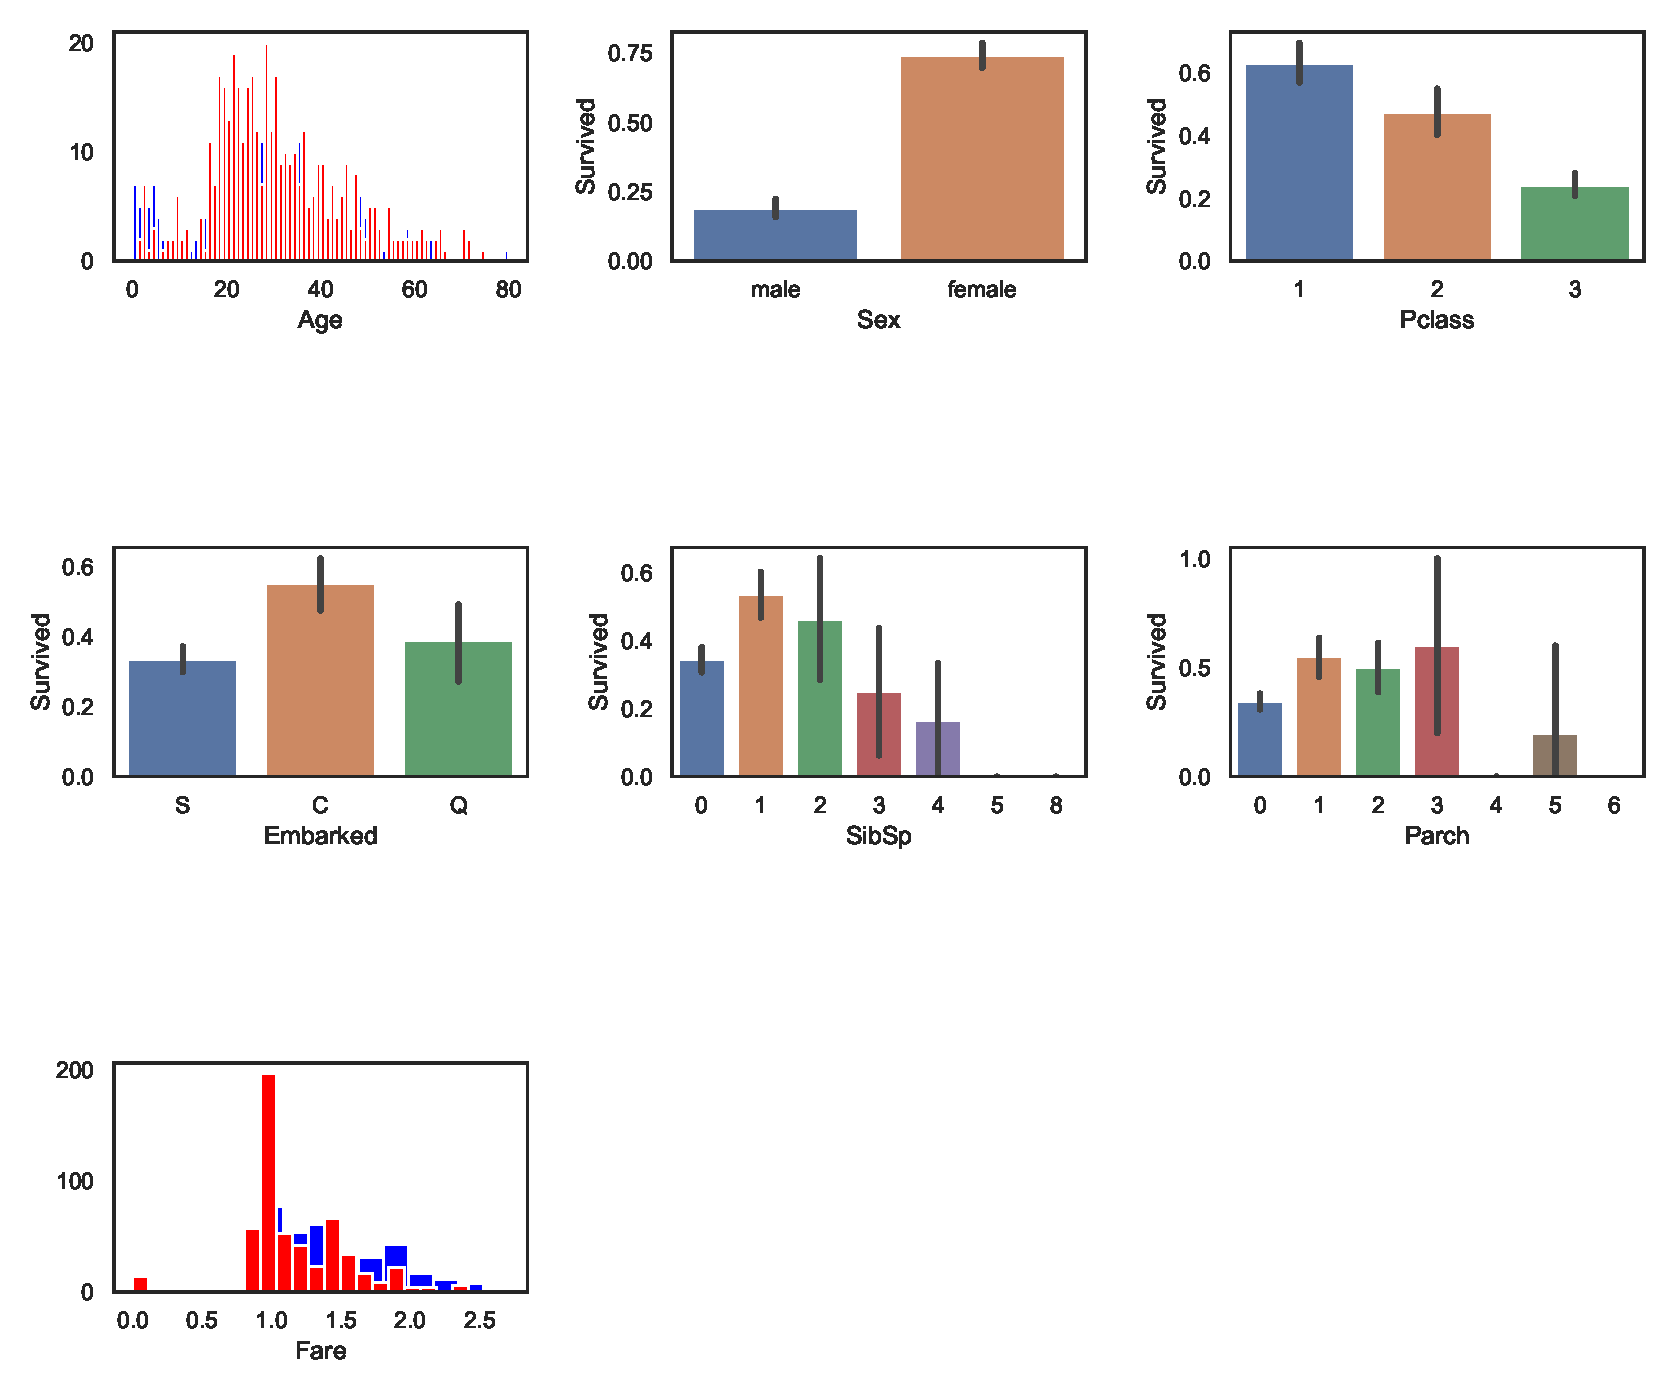
\includegraphics[width=1.0\textwidth,height=0.5\textwidth]{/Users/pratikshyaparajuli/Desktop/kaggle/KaggleProject/Code/templatex/graphics/titanicimg/allfeatures.eps}}
\end{figure}
\end{slide}
%DIF > %
%DIF > %
\begin{slide}[toc=,bm=]{Sex - Categorical Feature}
  \setlength{\abovecaptionskip}{0pt}
  \setlength{\belowcaptionskip}{10pt}
  \centering
  \begin{table}[tb]
    \setlength{\abovecaptionskip}{0pt}
    \setlength{\belowcaptionskip}{10pt}
    \centering
    \caption{\DIFaddFL{Survived vs. Sex}}

    \begin{tabular}{p{1.5cm}p{1.9cm}p{2.9cm}}
    \hline
      \DIFaddFL{Sex }\DIFaddendFL & \DIFdelbeginFL \texttt{\DIFdelFL{3PT\%}}  %DIFAUXCMD
\DIFdelendFL \DIFaddbeginFL \DIFaddFL{Survived }\DIFaddendFL & \DIFdelbeginFL \texttt{\DIFdelFL{FTA}} %DIFAUXCMD
\DIFdelendFL \DIFaddbeginFL \DIFaddFL{Numbers }\\
    \hline
      \DIFaddFL{Female   }\DIFaddendFL & \DIFdelbeginFL \texttt{\DIFdelFL{FT\%}} %DIFAUXCMD
\DIFdelendFL \DIFaddbeginFL \DIFaddFL{0    }\DIFaddendFL & \DIFdelbeginFL \texttt{\DIFdelFL{To}} %DIFAUXCMD
\DIFdelendFL \DIFaddbeginFL \DIFaddFL{81 }\DIFaddendFL \\
        \DIFdelbeginFL %DIFDELCMD < \midrule
%DIFDELCMD < %%%
\DIFdelFL{$P_1$
}\DIFdelendFL & \DIFdelbeginFL %DIFDELCMD < {%%%
\DIFdelFL{$65$}%DIFDELCMD < } %%%
\DIFdelendFL \DIFaddbeginFL \DIFaddFL{1 }\DIFaddendFL & \DIFdelbeginFL %DIFDELCMD < {%%%
\DIFdelFL{$4$}%DIFDELCMD < } %%%
\DIFdelendFL \DIFaddbeginFL \DIFaddFL{233 }\\
      \DIFaddFL{Male }\DIFaddendFL & \DIFdelbeginFL %DIFDELCMD < {%%%
\DIFdelFL{$33$}%DIFDELCMD < } %%%
\DIFdelendFL \DIFaddbeginFL \DIFaddFL{0  }\DIFaddendFL & \DIFdelbeginFL %DIFDELCMD < {%%%
\DIFdelFL{$8$}%DIFDELCMD < } %%%
\DIFdelendFL \DIFaddbeginFL \DIFaddFL{468 }\DIFaddendFL \\
        \DIFdelbeginFL \DIFdelFL{$P_2$
}\DIFdelendFL & \DIFdelbeginFL %DIFDELCMD < {%%%
\DIFdelFL{$78$}%DIFDELCMD < } %%%
\DIFdelendFL \DIFaddbeginFL \DIFaddFL{1  }\DIFaddendFL & \DIFdelbeginFL %DIFDELCMD < {%%%
\DIFdelFL{$1$}%DIFDELCMD < }%%%
\DIFdelendFL \DIFaddbeginFL \DIFaddFL{109  }\\
    \hline
    \end{tabular}
    \end{table}
    \begin{figure}
      \centering
      %DIF > \selectcolormodel{rgb}
      \centerline{\includegraphics[width=0.5\textwidth,height=.2\textwidth]{/Users/pratikshyaparajuli/Desktop/kaggle/KaggleProject/Code/templatex/graphics/titanicimg/survivedvsdead.eps}}
    \end{figure}
    \begin{itemize}
      \item
      \DIFadd{Survival rates for a women: \textcolor{orange}{75 percent and men: 18-19 percent}.
      }\end{itemize}
\end{slide}
%DIF > %
%DIF > %
\begin{slide}[toc=,bm=]{Pclass - Ordianal Feature}
  \setlength{\abovecaptionskip}{0pt}
  \setlength{\belowcaptionskip}{10pt}
  \centering
  \begin{table}[tb]
    \setlength{\abovecaptionskip}{0pt}
    \setlength{\belowcaptionskip}{10pt}
    \centering
    \caption{\DIFaddFL{Numbers of Passengers by Pclass}}

    \begin{tabular}{p{1.5cm}p{1.9cm}p{2.9cm}p{2.9cm}}
    \hline
    \DIFaddFL{Survived Pclass }\DIFaddendFL & \DIFdelbeginFL %DIFDELCMD < {%%%
\DIFdelFL{$65$}%DIFDELCMD < }%%%
\DIFdelendFL \DIFaddbeginFL \DIFaddFL{0 }\DIFaddendFL & \DIFdelbeginFL %DIFDELCMD < {%%%
\DIFdelFL{$5$}%DIFDELCMD < } %%%
\DIFdelendFL \DIFaddbeginFL \DIFaddFL{1 }& \DIFaddFL{All }\DIFaddendFL \\
    \DIFdelbeginFL \DIFdelFL{$P_3$
}\DIFdelendFL \DIFaddbeginFL \hline
      \DIFaddFL{1   }\DIFaddendFL & \DIFdelbeginFL %DIFDELCMD < {%%%
\DIFdelFL{$58$}%DIFDELCMD < } %%%
\DIFdelendFL \DIFaddbeginFL \DIFaddFL{80    }\DIFaddendFL & \DIFdelbeginFL %DIFDELCMD < {%%%
\DIFdelFL{$6$}%DIFDELCMD < } %%%
\DIFdelendFL \DIFaddbeginFL \DIFaddFL{136    }\DIFaddendFL &   \DIFdelbeginFL %DIFDELCMD < {%%%
\DIFdelFL{$46$}%DIFDELCMD < } &  {%%%
\DIFdelFL{$3$}%DIFDELCMD < } %%%
\DIFdelendFL \DIFaddbeginFL \DIFaddFL{216     }\DIFaddendFL \\
      \DIFdelbeginFL \DIFdelFL{$P_4$
}\DIFdelendFL \DIFaddbeginFL \DIFaddFL{2   }\DIFaddendFL & \DIFdelbeginFL %DIFDELCMD < {%%%
\DIFdelFL{$68$}%DIFDELCMD < } %%%
\DIFdelendFL \DIFaddbeginFL \DIFaddFL{97    }\DIFaddendFL & \DIFdelbeginFL %DIFDELCMD < {%%%
\DIFdelFL{$1.2$}%DIFDELCMD < }%%%
\DIFdelendFL \DIFaddbeginFL \DIFaddFL{87     }\DIFaddendFL &   \DIFdelbeginFL %DIFDELCMD < {%%%
\DIFdelFL{$85$}%DIFDELCMD < }&  {%%%
\DIFdelFL{$6.2$}%DIFDELCMD < } %%%
\DIFdelendFL \DIFaddbeginFL \DIFaddFL{184   }\DIFaddendFL \\
      \DIFdelbeginFL \DIFdelFL{$P_5$
}\DIFdelendFL \DIFaddbeginFL \DIFaddFL{3   }\DIFaddendFL & \DIFdelbeginFL %DIFDELCMD < {%%%
\DIFdelFL{$58$}%DIFDELCMD < } %%%
\DIFdelendFL \DIFaddbeginFL \DIFaddFL{372   }\DIFaddendFL & \DIFdelbeginFL %DIFDELCMD < {%%%
\DIFdelFL{$6.2$}%DIFDELCMD < } %%%
\DIFdelendFL \DIFaddbeginFL \DIFaddFL{119    }\DIFaddendFL &   \DIFdelbeginFL %DIFDELCMD < {%%%
\DIFdelFL{$36$}%DIFDELCMD < } %%%
\DIFdelendFL \DIFaddbeginFL \DIFaddFL{491  }\\
      \DIFaddFL{All }\DIFaddendFL & \DIFdelbeginFL %DIFDELCMD < {%%%
\DIFdelFL{$3.4$}%DIFDELCMD < }%%%
\DIFdelendFL \DIFaddbeginFL \DIFaddFL{549   }& \DIFaddFL{342    }&   \DIFaddFL{891 }\DIFaddendFL \\
    \DIFdelbeginFL %DIFDELCMD < \bottomrule
%DIFDELCMD < %%%
\DIFdelendFL \DIFaddbeginFL \hline
    \DIFaddendFL \end{tabular}
    \DIFdelbeginFL %DIFDELCMD < \end{center}
%DIFDELCMD < \bigskip
%DIFDELCMD < 

%DIFDELCMD < %%%
%DIF < %==========================================================================================
%DIFDELCMD < \begin{note}
%DIFDELCMD < %%%
\DIFdelFL{First, I will introduce the problem definition.
In the real life,
a teacher may be interested in the characteristics that
make one student obvious different from others.
Or,
NBA sports coaches would prefer to
know the advantages and disadvantages of one player.
Here, the player can be regarded as a query object.
}%DIFDELCMD < 

%DIFDELCMD < %%%
\DIFdelFL{For example, team A has five players,
each player has four features.
The NBA sports coaches may want to know the features of
player $1$ that are different from others.
}%DIFDELCMD < 

%DIFDELCMD < %%%
\DIFdelFL{The above example can be seen as outlying aspects mining.
The main purpose of outlying aspects mining is to identify
the outstanding features of the query object.
}%DIFDELCMD < \end{note}
%DIFDELCMD < %%%
%DIF < %==========================================================================================
%DIFDELCMD < 

%DIFDELCMD < %%%
\DIFdelendFL \DIFaddbeginFL \end{table}
    \vspace{0.2cm}
%DIF > \vspace{0.1cm}
\begin{figure}
  \centering
  %DIF > \selectcolormodel{rgb}
  \centerline{
    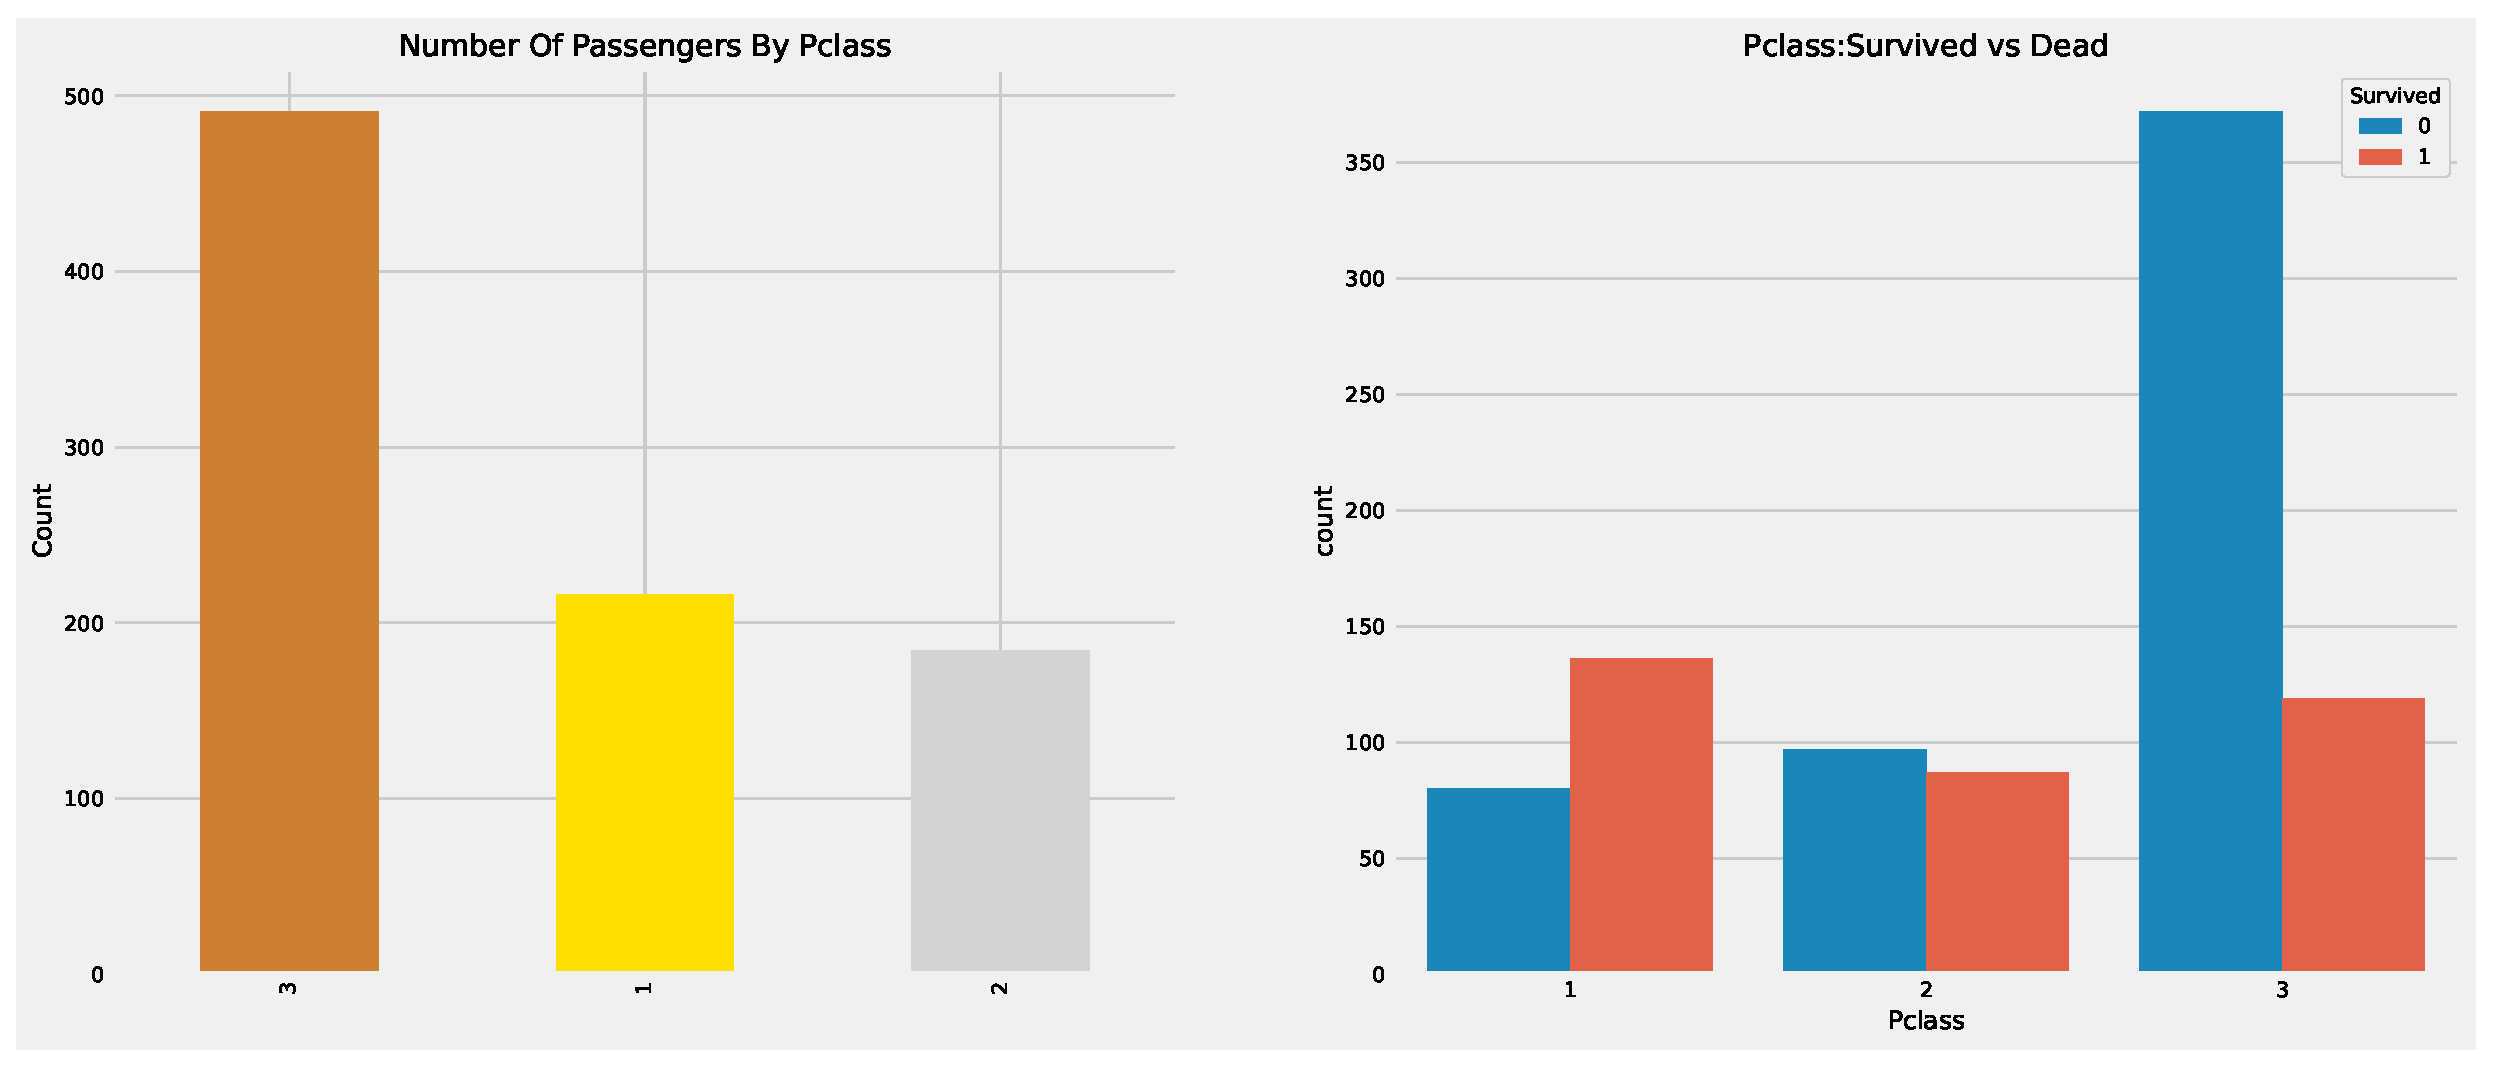
\includegraphics[width=0.5\textwidth,height=.2\textwidth]{/Users/pratikshyaparajuli/Desktop/kaggle/KaggleProject/Code/templatex/graphics/titanicimg/pclass.eps}
    }
    \caption{\DIFaddFL{Pclass:Survived vs Dead}}\label{fig:Pclass:Survived vs Dead}
\end{figure}
\DIFaddend \end{slide}
%%
%DIF < %==========================================================================================
\DIFdelbegin %DIFDELCMD < 

%DIFDELCMD < %%%
%DIF < %==========================================================================================
\DIFdelend %%
\DIFdelbegin %DIFDELCMD < \begin{slide}[toc=,bm=]{Outlying Aspects Mining vs Outlier Detection}
%DIFDELCMD < \begin{center}
%DIFDELCMD < \begin{tabular}{c| c c c c }
%DIFDELCMD < \toprule
%DIFDELCMD < %%%
%DIF < \centering
\DIFdel{Player }\DIFdelend \DIFaddbegin \begin{slide}[toc=,bm=]{Survival rate with Sex and Pclass Together}
  \setlength{\abovecaptionskip}{0pt}
  \setlength{\belowcaptionskip}{10pt}
  \centering
  \begin{table}[tb]
    \setlength{\abovecaptionskip}{0pt}
    \setlength{\belowcaptionskip}{10pt}
    \centering
    \caption{\DIFaddFL{Survival rate with Sex and Pclass Together}}

    \begin{tabular}{p{1.5cm}p{1.9cm}p{1.5cm}p{1.9cm}p{2.9cm}p{2.9cm}}
    \hline
     \DIFaddFL{Sex  }\DIFaddendFL & \DIFdelbeginFL \texttt{\DIFdelFL{3PT\%}}  %DIFAUXCMD
\DIFdelendFL \DIFaddbeginFL \DIFaddFL{PclassSurvived }\DIFaddendFL & \DIFdelbeginFL \texttt{\DIFdelFL{FTA}} %DIFAUXCMD
\DIFdelendFL \DIFaddbeginFL \DIFaddFL{1 }\DIFaddendFL & \DIFdelbeginFL \texttt{\DIFdelFL{FT\%}} %DIFAUXCMD
\DIFdelendFL \DIFaddbeginFL \DIFaddFL{2 }\DIFaddendFL &\DIFdelbeginFL \texttt{\DIFdelFL{To}} %DIFAUXCMD
\DIFdelendFL \DIFaddbeginFL \DIFaddFL{3  }& \DIFaddFL{All }\DIFaddendFL \\
    \DIFdelbeginFL %DIFDELCMD < \midrule
%DIFDELCMD < %%%
\DIFdelFL{$P_1$
}\DIFdelendFL \DIFaddbeginFL \hline
      \DIFaddFL{Female  }\DIFaddendFL & \DIFdelbeginFL %DIFDELCMD < {%%%
\DIFdelFL{$65$}%DIFDELCMD < } %%%
\DIFdelendFL \DIFaddbeginFL \DIFaddFL{0    }\DIFaddendFL & \DIFdelbeginFL %DIFDELCMD < {%%%
\DIFdelFL{$4$}%DIFDELCMD < } %%%
\DIFdelendFL \DIFaddbeginFL \DIFaddFL{3    }\DIFaddendFL &  \DIFdelbeginFL %DIFDELCMD < {%%%
\DIFdelFL{$33$}%DIFDELCMD < } %%%
\DIFdelendFL \DIFaddbeginFL \DIFaddFL{6    }\DIFaddendFL &  \DIFdelbeginFL %DIFDELCMD < {%%%
\DIFdelFL{$8$}%DIFDELCMD < } %%%
\DIFdelendFL \DIFaddbeginFL \DIFaddFL{72   }& \DIFaddFL{81  }\DIFaddendFL \\
              \DIFdelbeginFL \DIFdelFL{$P_2$
}\DIFdelendFL & \DIFdelbeginFL %DIFDELCMD < {%%%
\DIFdelFL{$78$}%DIFDELCMD < } %%%
\DIFdelendFL \DIFaddbeginFL \DIFaddFL{1    }\DIFaddendFL & \DIFdelbeginFL %DIFDELCMD < {%%%
\DIFdelFL{$1$}%DIFDELCMD < }%%%
\DIFdelendFL \DIFaddbeginFL \DIFaddFL{91   }\DIFaddendFL &  \DIFdelbeginFL %DIFDELCMD < {%%%
\DIFdelFL{$65$}%DIFDELCMD < }%%%
\DIFdelendFL \DIFaddbeginFL \DIFaddFL{70   }\DIFaddendFL &  \DIFdelbeginFL %DIFDELCMD < {%%%
\DIFdelFL{$5$}%DIFDELCMD < } %%%
\DIFdelendFL \DIFaddbeginFL \DIFaddFL{72   }& \DIFaddFL{233  }\DIFaddendFL \\
      \DIFdelbeginFL \DIFdelFL{$P_3$
}\DIFdelendFL \DIFaddbeginFL \DIFaddFL{Male    }\DIFaddendFL & \DIFdelbeginFL %DIFDELCMD < {%%%
\DIFdelFL{$58$}%DIFDELCMD < } %%%
\DIFdelendFL \DIFaddbeginFL \DIFaddFL{0    }\DIFaddendFL & \DIFdelbeginFL %DIFDELCMD < {%%%
\DIFdelFL{$6$}%DIFDELCMD < } %%%
\DIFdelendFL \DIFaddbeginFL \DIFaddFL{77   }\DIFaddendFL &  \DIFdelbeginFL %DIFDELCMD < {%%%
\DIFdelFL{$46$}%DIFDELCMD < } %%%
\DIFdelendFL \DIFaddbeginFL \DIFaddFL{91   }\DIFaddendFL &  \DIFdelbeginFL %DIFDELCMD < {%%%
\DIFdelFL{$3$}%DIFDELCMD < } %%%
\DIFdelendFL \DIFaddbeginFL \DIFaddFL{300  }& \DIFaddFL{468  }\DIFaddendFL \\
              \DIFdelbeginFL \DIFdelFL{$P_4$
}\DIFdelendFL & \DIFdelbeginFL %DIFDELCMD < {%%%
\DIFdelFL{$68$}%DIFDELCMD < } %%%
\DIFdelendFL \DIFaddbeginFL \DIFaddFL{1    }\DIFaddendFL & \DIFdelbeginFL %DIFDELCMD < {%%%
\DIFdelFL{$1.2$}%DIFDELCMD < }%%%
\DIFdelendFL \DIFaddbeginFL \DIFaddFL{45   }\DIFaddendFL &  \DIFdelbeginFL %DIFDELCMD < {%%%
\DIFdelFL{$85$}%DIFDELCMD < }%%%
\DIFdelendFL \DIFaddbeginFL \DIFaddFL{17   }\DIFaddendFL &  \DIFdelbeginFL %DIFDELCMD < {%%%
\DIFdelFL{$6.2$}%DIFDELCMD < } %%%
\DIFdelendFL \DIFaddbeginFL \DIFaddFL{47   }& \DIFaddFL{109  }\DIFaddendFL \\
      \DIFdelbeginFL \DIFdelFL{$P_5$
}\DIFdelendFL \DIFaddbeginFL \DIFaddFL{All     }\DIFaddendFL &      \DIFdelbeginFL %DIFDELCMD < {%%%
\DIFdelFL{$58$}%DIFDELCMD < } %%%
\DIFdelendFL & \DIFdelbeginFL %DIFDELCMD < {%%%
\DIFdelFL{$6.2$}%DIFDELCMD < } %%%
\DIFdelendFL \DIFaddbeginFL \DIFaddFL{216  }\DIFaddendFL &  \DIFdelbeginFL %DIFDELCMD < {%%%
\DIFdelFL{$36$}%DIFDELCMD < } %%%
\DIFdelendFL \DIFaddbeginFL \DIFaddFL{184  }\DIFaddendFL &  \DIFdelbeginFL %DIFDELCMD < {%%%
\DIFdelFL{$3.4$}%DIFDELCMD < }%%%
\DIFdelendFL \DIFaddbeginFL \DIFaddFL{491  }& \DIFaddFL{891  }\DIFaddendFL \\
    \DIFdelbeginFL %DIFDELCMD < \bottomrule
%DIFDELCMD < %%%
\DIFdelendFL \DIFaddbeginFL \hline
    \DIFaddendFL \end{tabular}
    \DIFdelbeginFL %DIFDELCMD < \end{center}
%DIFDELCMD < 

%DIFDELCMD < \bigskip
%DIFDELCMD < 

%DIFDELCMD < \twocolumn[
%DIFDELCMD < \savevalue{lfrheight}=4.6cm,
%DIFDELCMD < \savevalue{lfrprop}={
%DIFDELCMD < linestyle=solid,framearc=.2,linewidth=1pt},
%DIFDELCMD < rfrheight=\usevalue{lfrheight},
%DIFDELCMD < rfrprop=\usevalue{lfrprop}
%DIFDELCMD < ]{
%DIFDELCMD < Outlying Aspects Mining
%DIFDELCMD < \begin{itemize}
\begin{itemize}%DIFAUXCMD
%DIFDELCMD < \item
\item%DIFAUXCMD
%DIFDELCMD < \smallskip
%DIFDELCMD < Explain the distinctive \textcolor{orange}{aspects} of the query object.
%DIFDELCMD < \smallskip
%DIFDELCMD < \item
\item%DIFAUXCMD
%DIFDELCMD < \smallskip
%DIFDELCMD < The query object may (or may not) be an outlier.

\end{itemize}%DIFAUXCMD
%DIFDELCMD < \end{itemize}
%DIFDELCMD < }{
%DIFDELCMD < Outlier Detection
%DIFDELCMD < \begin{itemize}
\begin{itemize}%DIFAUXCMD
%DIFDELCMD < \item
\item%DIFAUXCMD
%DIFDELCMD < \smallskip
%DIFDELCMD < Find out \textcolor{orange}{all} unusual
%DIFDELCMD < \textcolor{orange}{objects} in the whole dataset.
%DIFDELCMD < \smallskip
%DIFDELCMD < \item
\item%DIFAUXCMD
%DIFDELCMD < \smallskip
%DIFDELCMD < \textcolor{orange}{No} explanation on how they are different.

\end{itemize}%DIFAUXCMD
%DIFDELCMD < \end{itemize}
%DIFDELCMD < }
%DIFDELCMD < 

%DIFDELCMD < %%%
%DIF < %==========================================================================================
%DIFDELCMD < \begin{note}
%DIFDELCMD < %%%
\DIFdelFL{Based on the above example,
I will compare the differences
between outlying aspects mining and outlier detection.
}%DIFDELCMD < 

%DIFDELCMD < %%%
\DIFdelFL{Outlying aspects mining aims to
explain the distinctive aspects of the query object.
The query object may or may not be an outlier.
In contrast,
Outlier detection aims to discover all possible
outlying objects in the dataset.
Without explaining how and why they are different.
}%DIFDELCMD < 

%DIFDELCMD < %%%
\DIFdelFL{Let's go back to the NBA example,
in that example,
the output of the outlying aspects mining may be
a combination of four features,
but the output of the outlier detection may be any of those five players.
}%DIFDELCMD < \end{note}
%DIFDELCMD < %%%
%DIF < %==========================================================================================
%DIFDELCMD < 

%DIFDELCMD < \end{slide}
%DIFDELCMD < %%%
%DIF < %
%DIF < %==========================================================================================
%DIFDELCMD < 

%DIFDELCMD < %%%
%DIF < %==========================================================================================
%DIF < %
%DIFDELCMD < \begin{slide}{Group Outlying Aspects Mining}
%DIFDELCMD < \twotonebox {\rotatebox{90}{Defn}}{%%%
\parbox{\DIFdelFL{.88\textwidth}}
%DIFAUXCMD
%DIFDELCMD < {
%DIFDELCMD < {%%%
\DIFdelFL{\textcolor{orange}{Group outlying aspects mining} aims to
identify the outstanding features of the group of query object.
}%DIFDELCMD < \begin{itemize}
\begin{itemize}%DIFAUXCMD
%DIFDELCMD < \item
\item%DIFAUXCMD
%DIFDELCMD < %%%
\DIFdelFL{Doctors desire to identify the merits \& demerits between
\textcolor{orange}{a group of cancer patients} and normal people.
    \item
NBA coaches are passionate about exploring the obvious advantages \&
disadvantages of \textcolor{orange}{the team}.
\end{itemize}
}
}%DIFDELCMD < }}
%DIFDELCMD < 

%DIFDELCMD < \vspace{1.5cm}
%DIFDELCMD < 

%DIFDELCMD < \twocolumn{
%DIFDELCMD < \begin{figure}
%DIFDELCMD <   \centering
%DIFDELCMD <   \selectcolormodel{rgb}
%DIFDELCMD <   \missingfigure{Testing.}
%DIFDELCMD <   %\includegraphics[width=0.6\textwidth]{figures//demical.eps}\\
%DIFDELCMD <   \caption{Medical}\label{fig:demical}
%DIFDELCMD < \end{figure}
%DIFDELCMD < }{
%DIFDELCMD < \begin{figure}
%DIFDELCMD <   \centering
%DIFDELCMD <   \selectcolormodel{rgb}
%DIFDELCMD <   \missingfigure{Testing.}
%DIFDELCMD <   %\includegraphics[width=0.6\textwidth]{figures//NBA_team.eps}\\
%DIFDELCMD <   \caption{NBA-Team}\label{fig:timg}
%DIFDELCMD < \end{figure}
%DIFDELCMD < }
%DIFDELCMD < 

%DIFDELCMD < %%%
%DIF < %==========================================================================================
%DIFDELCMD < \begin{note}
%DIFDELCMD < %%%
\DIFdelFL{However,
there is such a phenomenon in real life.
Doctors desire to identify the characteristics between
a group of cancer patients and normal people.
NBA coaches are passionate about exploring the obvious strengths and
weaknesses of the team compared with other teams.
}%DIFDELCMD < 

%DIFDELCMD < %%%
\DIFdelFL{Based on such a phenomenon in the real life,
we proposed the concept of group outlying aspects mining.
}%DIFDELCMD < \end{note}
%DIFDELCMD < %%%
%DIF < %==========================================================================================
%DIFDELCMD < 

%DIFDELCMD < \end{slide}
%DIFDELCMD < %%%
%DIF < %
%DIF < %==========================================================================================
%DIFDELCMD < 

%DIFDELCMD < %%%
%DIF < %==========================================================================================
%DIF < %
%DIFDELCMD < \begin{slide}[toc=,bm=]{Problem Formalization}
%DIFDELCMD < \twotonebox {\rotatebox{90}{Defn}}{%%%
\parbox{\DIFdelFL{.88\textwidth}}
%DIFAUXCMD
%DIFDELCMD < {
%DIFDELCMD < {%%%
\DIFdelFL{\textcolor{orange}{Group outlying aspects mining} aims to identify
the \textcolor{orange}{top-k group outlying subspace $s \subseteq F$} in
which the query group $G_q$ is \textcolor{orange} }%DIFDELCMD < {%%%
\DIFdelFL{distinctive with other groups}%DIFDELCMD < }%%%
\DIFdelFL{.
}%DIFDELCMD < \begin{itemize}
%DIFDELCMD < \item
%DIFDELCMD < %%%
\DIFdelFL{$G = \{G_q, G_2, G_3,..., G_n\}$ $\Leftrightarrow$ a set of groups.
}%DIFDELCMD < \item
%DIFDELCMD < %%%
\DIFdelFL{$G_q$ $\Leftrightarrow$ the query group.
}%DIFDELCMD < \item
%DIFDELCMD < %%%
\DIFdelFL{Other groups $\Leftrightarrow$ comparison groups.
}%DIFDELCMD < \item
%DIFDELCMD < %%%
\DIFdelFL{Each object in the group has $d$ features $F = \{f_1, f_2, ..., f_d\}$.
}
\end{itemize}%DIFAUXCMD
%DIFDELCMD < \end{itemize}
%DIFDELCMD < }
%DIFDELCMD < }}
%DIFDELCMD < 

%DIFDELCMD < %%%
%DIF < %==========================================================================================
%DIFDELCMD < \begin{note}
%DIFDELCMD < %%%
\DIFdelFL{Next,
let me talk about the concept of group outlying aspects mining.
}%DIFDELCMD < 

%DIFDELCMD < %%%
\DIFdelFL{For example,
Dataset $G$ has $n$ groups.
$G_q$ is the query group. and other groups are comparison groups.
Each object in the group has d features $F = $ $f_1$, $f_2$, $f_3$ to $f_d$.
The group outlying aspects mining is to identify the top-k group outlying subspaces,which are different from other groups.
    }%DIFDELCMD < 

%DIFDELCMD < %%%
\DIFdelFL{What does the top-k group outlying subspaces mean?
Next, I will explain it.
}%DIFDELCMD < \end{note}
%DIFDELCMD < 

%DIFDELCMD < %%%
%DIF < %==========================================================================================
%DIFDELCMD < \end{slide}
%DIFDELCMD < %%%
%DIF < %
%DIF < %==========================================================================================
%DIFDELCMD < 

%DIFDELCMD < %%%
%DIF < %==========================================================================================
%DIF < %
%DIFDELCMD < \begin{slide}[toc=,bm=]{Term Definition}
%DIFDELCMD < \begin{itemize}
\begin{itemize}%DIFAUXCMD
%DIFDELCMD < \item
\item%DIFAUXCMD
%DIFDELCMD < %%%
\DIFdelFL{Top-k group outlying subspaces
}%DIFDELCMD < 

%DIFDELCMD < \begin{itemize}
%DIFDELCMD < \item
\item%DIFAUXCMD
%DIFDELCMD < %%%
\DIFdelFL{$\rho_s(\cdot)$ $\Rightarrow$ outlying scoring function.
}%DIFDELCMD < 

%DIFDELCMD < \item
\item%DIFAUXCMD
%DIFDELCMD < %%%
\DIFdelFL{$\rho_s(\cdot)$ quantifies the outlying degree of the
query group $G_q$ in the subspace $s$.
}%DIFDELCMD < 

%DIFDELCMD < \item
\item%DIFAUXCMD
%DIFDELCMD < %%%
\DIFdelFL{Order by DESC using scoring function $\rho(\cdot)$
to identify top K group outlying subspaces.
}
\end{itemize}%DIFAUXCMD
%DIFDELCMD < \end{itemize}
%DIFDELCMD < \end{itemize}
%DIFDELCMD < 

%DIFDELCMD < \begin{figure}[htbp]
%DIFDELCMD <     %%%
\DIFdelendFL \DIFaddbeginFL \end{table}
    \vspace{0.1cm}
%DIF > \vspace{0.1cm}
\begin{figure}
  \DIFaddendFL \centering
  \DIFdelbeginFL %DIFDELCMD < \subfigure[Original Feature Spaces]{
%DIFDELCMD <       \selectcolormodel{rgb}
%DIFDELCMD <       \missingfigure[figwidth=5.5cm]{Test.}
%DIFDELCMD <         %\includegraphics[width=0.3\textwidth]{figures//example-basketball-original.eps}
%DIFDELCMD <         \label{fig:basketball-original}
%DIFDELCMD <     }
%DIFDELCMD <     \subfigure[Group Outlying Spaces]{
%DIFDELCMD <        \selectcolormodel{rgb}
%DIFDELCMD <        \missingfigure[figwidth=5.5cm]{Test.}
%DIFDELCMD <         %\includegraphics[width=0.3\textwidth]{figures//example-basketball-projection.eps}
%DIFDELCMD <         \label{fig:basketball-projection}
%DIFDELCMD <     }
%DIFDELCMD <     \subfigure[Another Subspaces]{
%DIFDELCMD <       \selectcolormodel{rgb}
%DIFDELCMD <       \missingfigure[figwidth=5.5cm]{Test.}
%DIFDELCMD <         %\includegraphics[width=0.28\textwidth]{figures//basketball-another-subspaces.eps}
%DIFDELCMD <         \label{fig:basketball-projection1}
%DIFDELCMD <     }
%DIFDELCMD < %%%
%DIF <     \caption{Histogram representation of a group on three single features}
    %DIFDELCMD < \label{fig:Basketball-Example}
%DIFDELCMD < %%%
\DIFdelendFL %DIF > \selectcolormodel{rgb}
  %DIF > \missingfigure{Testing a long text string.}
  \DIFaddbeginFL \centerline{
    \includegraphics[width=0.5\textwidth,height=.2\textwidth]{/Users/pratikshyaparajuli/Desktop/kaggle/KaggleProject/Code/templatex/graphics/titanicimg/pclassvssex.eps}
    }
  \caption{\DIFaddFL{Survival rate with Sex and Pclass Together}}\label{fig:sexvspclass}
\DIFaddendFL \end{figure}
\DIFdelbegin %DIFDELCMD < 

%DIFDELCMD < %%%
%DIF < %==========================================================================================
%DIFDELCMD < \begin{note}
%DIFDELCMD < %%%
\DIFdel{We use $\rho_s(\cdot)$ to describe an outlying scoring function.
$\rho_s(\cdot)$ quantifies the outlying degree of the query group in a subspaces $s$.
In addition,
we use the scoring function to make a descending order and at last
filter out the top k group outlying subspaces.
It is obvious that the outlying subspaces make the
query group different from other groups.
}%DIFDELCMD < \end{note}
%DIFDELCMD < %%%
%DIF < %==========================================================================================
%DIFDELCMD < 

%DIFDELCMD < %%%
\DIFdelend \end{slide}
%%
%DIF < %==========================================================================================
\DIFdelbegin %DIFDELCMD < 

%DIFDELCMD < %%%
%DIF < %==========================================================================================
\DIFdelend %%
\DIFdelbegin %DIFDELCMD < \begin{slide}[toc=,bm=]{Term Definition}
%DIFDELCMD < \begin{itemize}
\begin{itemize}%DIFAUXCMD
%DIFDELCMD < \item
\item%DIFAUXCMD
%DIFDELCMD < %%%
\DIFdel{Trivial Outlying Features
}%DIFDELCMD < 

%DIFDELCMD < \begin{itemize}
%DIFDELCMD < \item
\item%DIFAUXCMD
%DIFDELCMD < \smallskip
%DIFDELCMD < %%%
\DIFdel{One-dimension subspaces.
      }%DIFDELCMD < 

%DIFDELCMD < \item
\item%DIFAUXCMD
%DIFDELCMD < %%%
\DIFdel{${G_q}$'s outlying degree $\rho(\cdot)$ $>$ $\alpha$.
}
\end{itemize}%DIFAUXCMD
%DIFDELCMD < \end{itemize}
%DIFDELCMD < \end{itemize}
%DIFDELCMD < \begin{table}
%DIFDELCMD < \setlength{\abovecaptionskip}{0pt}
%DIFDELCMD < \setlength{\belowcaptionskip}{10pt}
%DIFDELCMD < %%%
\DIFdelendFL \DIFaddbeginFL \begin{slide}[toc=,bm=]{Age - Continuous Feature}
  \DIFaddFL{Oldest Passenger was of: 80.0 Years }\\
  \DIFaddFL{Youngest Passenger was of: 0.42 Years 
}\vspace{0.1cm}
\begin{figure}
  \DIFaddendFL \centering
  \DIFdelbeginFL %DIFDELCMD < \caption{%
{%DIFAUXCMD
\DIFdelFL{$\alpha = 4$}}
%DIFAUXCMD
%DIFDELCMD < 

%DIFDELCMD < \begin{tabular}{  c  |  c }
%DIFDELCMD < \toprule
%DIFDELCMD < \centering
%DIFDELCMD < %%%
\texttt{\DIFdelFL{Feature}}  %DIFAUXCMD
%DIFDELCMD < & %%%
\texttt{\DIFdelFL{Outlying Degree}}  %DIFAUXCMD
\DIFdelendFL %DIF > \selectcolormodel{rgb}
  %DIF > \missingfigure{Testing a long text string.}
  \DIFaddbeginFL \centerline{
    \includegraphics[width=0.6\textwidth,height=.2\textwidth]{/Users/pratikshyaparajuli/Desktop/kaggle/KaggleProject/Code/templatex/graphics/titanicimg/age.eps}
    }
  \caption{\DIFaddFL{Survival rate with Age }}\label{fig:age}
\end{figure}
\DIFaddFL{\textcolor{orange}{Observations:}}\DIFaddendFL \\
\DIFdelbeginFL %DIFDELCMD < \midrule
%DIFDELCMD <  {%%%
\DIFdelFL{\textcolor{orange}{\{$F_1$\}}}%DIFDELCMD < } & %%%
\DIFdelFL{$4.351$ }\DIFdelendFL \DIFaddbeginFL \DIFaddFL{1)The Toddlers(age<5) were saved in large numbers.}\DIFaddendFL \\
\DIFdelbeginFL %DIFDELCMD < {%%%
\DIFdelFL{\{$F_3, F_4$\}}%DIFDELCMD < }                & %%%
\DIFdelFL{$4.024$ }%DIFDELCMD < \\
%DIFDELCMD <  {%%%
\DIFdelFL{\{$F_2, F_4$\}}%DIFDELCMD < }                & %%%
\DIFdelFL{$2.318$ }%DIFDELCMD < \\
%DIFDELCMD <  {%%%
\DIFdelFL{\{$F_2$\}}%DIFDELCMD < }                     & %%%
\DIFdelFL{$2.002$ }%DIFDELCMD < \\
%DIFDELCMD <  {%%%
\DIFdelFL{\{$F_3$\}}%DIFDELCMD < }                     & %%%
\DIFdelFL{$1.028$ }%DIFDELCMD < \\
%DIFDELCMD < \bottomrule
%DIFDELCMD < \end{tabular}
%DIFDELCMD < \end{table}
%DIFDELCMD < 

%DIFDELCMD < %%%
%DIF < %==========================================================================================
%DIFDELCMD < \begin{note}
%DIFDELCMD < %%%
\DIFdel{In order to identify the top-k outlying subspaces,
we categorize the features into $2$ non-overlapping groups,
trivial outlying features and non-trivial outlying subspaces.
}%DIFDELCMD < 

%DIFDELCMD < %%%
\DIFdel{First, let me introduce the trivial outlying features.
}%DIFDELCMD < 

%DIFDELCMD < %%%
\DIFdel{Trivial outlying features are one-dimension subspaces.
In the subspace,
the query group's outlying degree is larger than the threshold $\alpha$}\DIFdelend \DIFaddbegin \DIFadd{2)The oldest Passenger was saved(80 years)}\DIFaddend .\DIFdelbegin %DIFDELCMD < 

%DIFDELCMD < %%%
\DIFdel{We can see from table $1$,
when the specified threshold $\alpha = 4$,
the trivial outlying feature is \{$F_1$\}.
}%DIFDELCMD < \end{note}
%DIFDELCMD < %%%
%DIF < %==========================================================================================
%DIFDELCMD < 

%DIFDELCMD < %%%
\DIFdelend \DIFaddbegin \\
\DIFadd{3)Maximum number of deaths were in the age group of 30-40.
}\DIFaddend \end{slide}
%%
%DIF < %==========================================================================================
\DIFdelbegin %DIFDELCMD < 

%DIFDELCMD < %%%
%DIF < %==========================================================================================
\DIFdelend %%
\DIFdelbegin %DIFDELCMD < \begin{slide}[toc=,bm=]{Term Definition}
%DIFDELCMD < \begin{itemize}
\begin{itemize}%DIFAUXCMD
%DIFDELCMD < \item
\item%DIFAUXCMD
%DIFDELCMD < %%%
\DIFdel{Non-Trivial Outlying Subspaces
}%DIFDELCMD < \begin{itemize}
%DIFDELCMD < \item
\item%DIFAUXCMD
%DIFDELCMD < \smallskip
%DIFDELCMD < %%%
\DIFdel{Multi-dimension subspaces.
}%DIFDELCMD < 

%DIFDELCMD < \item
\item%DIFAUXCMD
%DIFDELCMD < \smallskip
%DIFDELCMD < %%%
\DIFdel{${G_q}$'s outlying degree $\rho(\cdot)$ $>$ $\alpha$.
}
\end{itemize}%DIFAUXCMD
%DIFDELCMD < \end{itemize}
%DIFDELCMD < \end{itemize}
%DIFDELCMD < 

%DIFDELCMD < \begin{table}
%DIFDELCMD < \setlength{\abovecaptionskip}{0pt}
%DIFDELCMD < \setlength{\belowcaptionskip}{10pt}
%DIFDELCMD < \centering
%DIFDELCMD < %%%
%DIFDELCMD < \caption{%
{%DIFAUXCMD
\DIFdelFL{$\alpha = 4$}}
%DIFAUXCMD
%DIFDELCMD < 

%DIFDELCMD < \begin{tabular}{  c  |  c }
%DIFDELCMD < \toprule
%DIFDELCMD < \centering
%DIFDELCMD < %%%
\texttt{\DIFdelFL{Feature}}  %DIFAUXCMD
%DIFDELCMD < & %%%
\texttt{\DIFdelFL{Outlying Degree}}  %DIFAUXCMD
\DIFdelendFL \DIFaddbeginFL \begin{slide}[toc=,bm=]{Embarked - Categorical Value}
  \DIFaddFL{1)Maximum passenegers boarded from S. Majority of them being from Pclass3.}\DIFaddendFL \\
\DIFdelbeginFL %DIFDELCMD < \midrule
%DIFDELCMD <  {%%%
\DIFdelFL{\{$F_1$\}}%DIFDELCMD < }                           & %%%
\DIFdelFL{$4.351$ }\DIFdelendFL \DIFaddbeginFL \DIFaddFL{2)The Passengers from C survived. }\DIFaddendFL \\
\DIFdelbeginFL %DIFDELCMD < {%%%
\DIFdelFL{\textcolor{orange}{\{$F_3, F_4$\}}}%DIFDELCMD < }  & %%%
\DIFdelFL{$4.024$ }\DIFdelendFL \DIFaddbeginFL \DIFaddFL{3)The Embark S looks to the port from where majority of the rich people boarded. Still the chances for survival is low here.}\DIFaddendFL \\
\DIFdelbeginFL %DIFDELCMD < {%%%
\DIFdelFL{\{$F_2, F_4$\}}%DIFDELCMD < }                      & %%%
\DIFdelFL{$2.318$ }%DIFDELCMD < \\
%DIFDELCMD <  {%%%
\DIFdelFL{\{$F_2$\}}%DIFDELCMD < }                           & %%%
\DIFdelFL{$2.002$ }%DIFDELCMD < \\
%DIFDELCMD <  {%%%
\DIFdelFL{\{$F_3$\}}%DIFDELCMD < }                           & %%%
\DIFdelFL{$1.028$ }%DIFDELCMD < \\
%DIFDELCMD < \bottomrule
%DIFDELCMD < \end{tabular}
%DIFDELCMD < \end{table}
%DIFDELCMD < %%%
\DIFdelend \DIFaddbegin \DIFadd{4)Port Q had almost 95 percent of the passengers were from Pclass3.
}\vspace{0.1cm}
\begin{figure}
  \centering
  \centerline{
    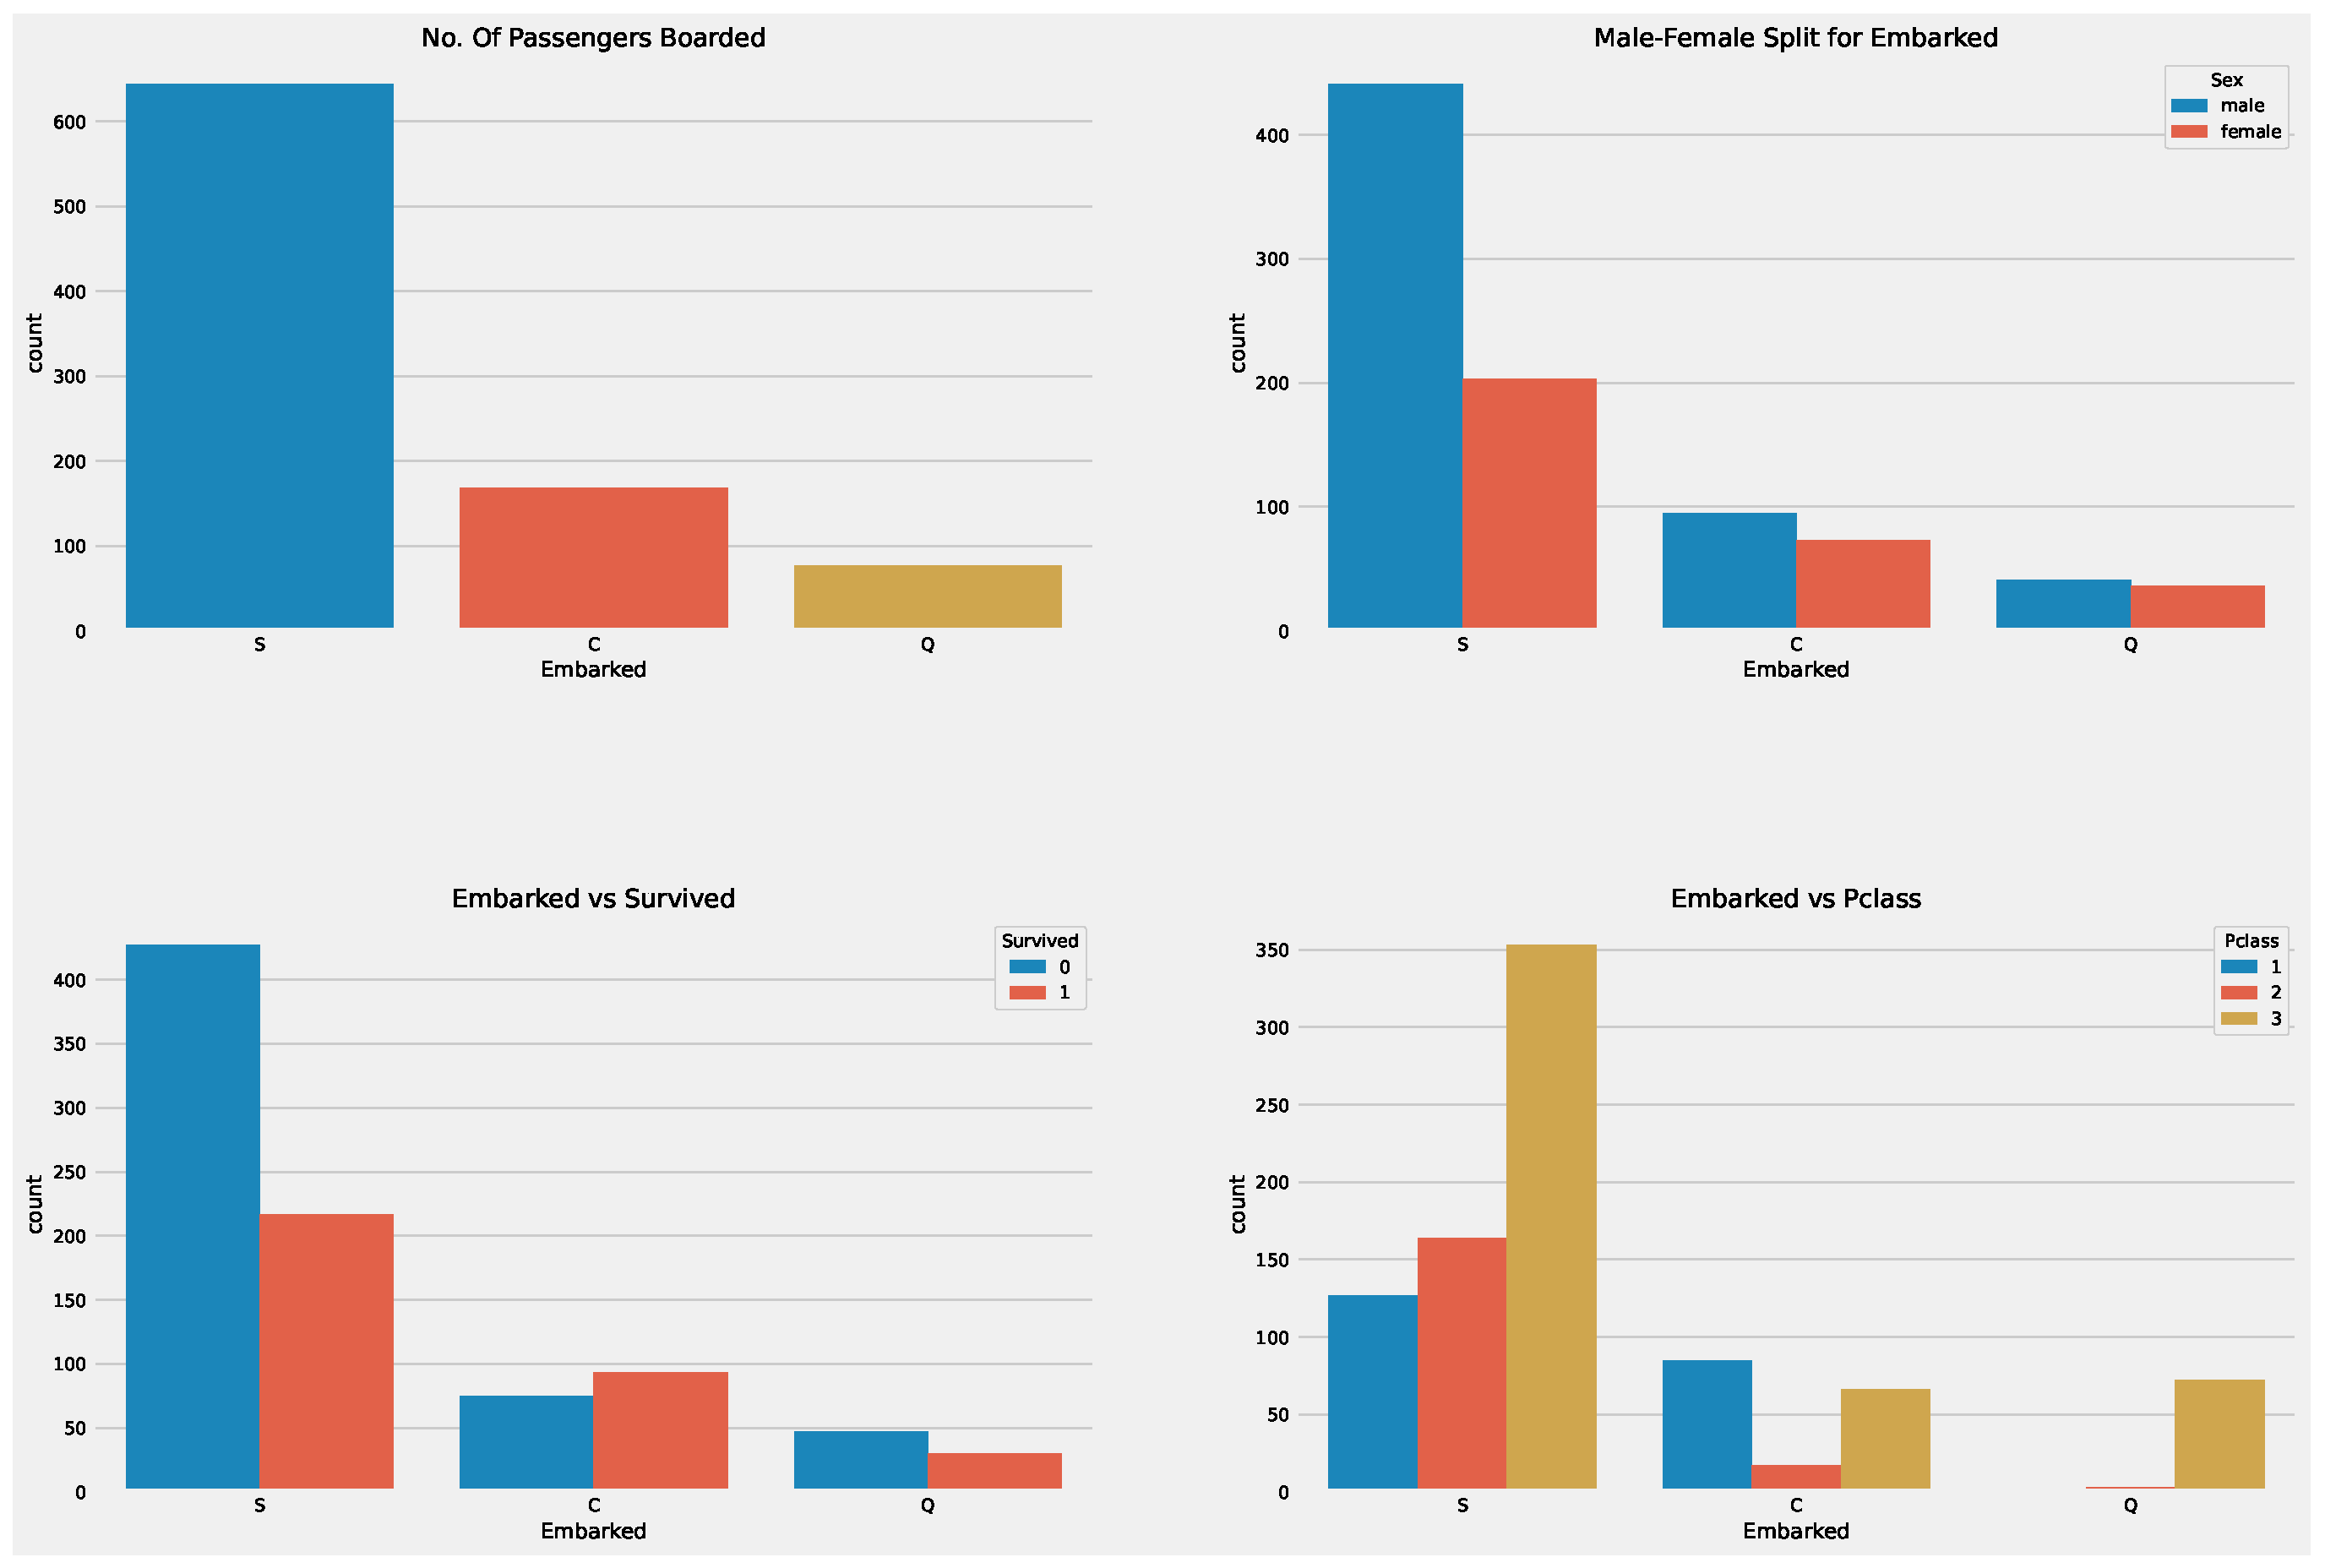
\includegraphics[width=0.6\textwidth,height=.3\textwidth]{/Users/pratikshyaparajuli/Desktop/kaggle/KaggleProject/Code/templatex/graphics/titanicimg/embark.eps}
    }
  \caption{\DIFaddFL{Survival rate with Port of Embarkation}}\label{fig:embark}
\end{figure}
\DIFaddend 

%DIF < %==========================================================================================
\DIFdelbegin %DIFDELCMD < \begin{note}
%DIFDELCMD < %%%
\DIFdel{Next,
I will introduce the non-trivial outlying subspaces.
Non-Trivial outlying subspaces are multi-dimension subspaces.
In the subspace,
the query group's outlying degree is larger than the threshold $\alpha$.
}%DIFDELCMD < 

%DIFDELCMD < %%%
\DIFdel{Table $2$ shows that,
when the threshold $\alpha$ equal four,
the non-trivial outlying subspace is \{$F_3$, $F_4$\}.
}%DIFDELCMD < \end{note}
%DIFDELCMD < %%%
%DIF < %==========================================================================================
%DIFDELCMD < 

%DIFDELCMD < %%%
\DIFdelend \end{slide}
%%
%DIF < %==========================================================================================
\DIFdelbegin %DIFDELCMD < 

%DIFDELCMD < %%%
\section{\DIFdel{Related Work and Challenges}}
%DIFAUXCMD
\addtocounter{section}{-1}%DIFAUXCMD
%DIFDELCMD < 

%DIFDELCMD < %%%
%DIF < %==========================================================================================
\DIFdelend %%
\DIFdelbegin %DIFDELCMD < \begin{slide}{Related Work - Outlying Aspects Mining}
%DIFDELCMD < %%%
%DIF < Related Work - Outlying Aspects Mining
%DIFDELCMD < \begin{itemize}
\begin{itemize}%DIFAUXCMD
%DIFDELCMD < \item
\item%DIFAUXCMD
%DIFDELCMD < %%%
\DIFdel{Existing Methods - \textcolor{orange}{Feature selection}
}%DIFDELCMD < 

%DIFDELCMD < \begin{itemize}
%DIFDELCMD < \item
\item%DIFAUXCMD
%DIFDELCMD < %%%
\DIFdel{To distinguish two classes: the query point (positive) \& rest of data (negative)}
\end{itemize}%DIFAUXCMD
%DIFDELCMD < \end{itemize}
%DIFDELCMD < \vspace{1cm}
%DIFDELCMD < \twocolumn[
%DIFDELCMD < \savevalue{lfrheight}=5cm,
%DIFDELCMD < \savevalue{lfrprop}={
%DIFDELCMD < linestyle=solid,framearc=.2,linewidth=1pt},
%DIFDELCMD < rfrheight=\usevalue{lfrheight},
%DIFDELCMD < rfrprop=\usevalue{lfrprop}
%DIFDELCMD < ]{
%DIFDELCMD < Disadvantages
%DIFDELCMD < \begin{itemize}
\begin{itemize}%DIFAUXCMD
%DIFDELCMD < \item
\item%DIFAUXCMD
%DIFDELCMD < \smallskip
%DIFDELCMD < Positive and negative classes are \textcolor{orange}{Not} balanced.
%DIFDELCMD < 

%DIFDELCMD < \item
\item%DIFAUXCMD
%DIFDELCMD < \smallskip
%DIFDELCMD < \textcolor{orange}{Not} quantify the outlying degree accurately.
%DIFDELCMD < 

%DIFDELCMD < \item
\item%DIFAUXCMD
%DIFDELCMD < \smallskip
%DIFDELCMD < \textcolor{orange}{Not} identify group outlying aspects.

\end{itemize}%DIFAUXCMD
%DIFDELCMD < \end{itemize}
%DIFDELCMD < }
%DIFDELCMD < {
%DIFDELCMD < %%%
\DIFdel{Advantages
}%DIFDELCMD < \begin{itemize}
\begin{itemize}%DIFAUXCMD
%DIFDELCMD < \item
\item%DIFAUXCMD
%DIFDELCMD < \smallskip
%DIFDELCMD < %%%
\DIFdel{Easy to operate.}%DIFDELCMD < 

%DIFDELCMD < \item
\item%DIFAUXCMD
%DIFDELCMD < \smallskip
%DIFDELCMD < %%%
\DIFdel{Resolve dimensionality bias.
}
\end{itemize}%DIFAUXCMD
%DIFDELCMD < \end{itemize}
%DIFDELCMD < }
%DIFDELCMD < \end{itemize}
%DIFDELCMD < 

%DIFDELCMD < %%%
%DIF < %==========================================================================================
%DIFDELCMD < \begin{note}
%DIFDELCMD < %%%
\DIFdel{Let me introduce two existing methods:
Feature selection and score-and-search.
}%DIFDELCMD < 

%DIFDELCMD < %%%
\DIFdel{For feature selection,
the query point can be regarded as positive class and
the rest of the data can be regarded as negative class,
selected the features that best distinguish the two classes.
}%DIFDELCMD < 

%DIFDELCMD < %%%
\DIFdel{The advantages of this method are easy to operate,
and it's able to resolve dimensionality bias.
However, it has some drawbacks.
Firstly,
positive and negative classes are Not balanced,
secondly,
it can't quantify the outlying degree correctly.
Most importantly,
it doesn't identify group outlying aspects.
}%DIFDELCMD < \end{note}
%DIFDELCMD < %%%
%DIF < %==========================================================================================
%DIFDELCMD < 

%DIFDELCMD < \end{slide}
%DIFDELCMD < %%%
\DIFdelend %DIF >  \begin{slide}[toc=,bm=]{SibSip - Discrete Feature}
%DIF >    This feature represents whether a person is alone or with his family members.\\
%DIF >    Sibling = brother, sister, stepbrother, stepsister\\
%DIF >    Spouse = husband, wife\\
%DIF >    insert figure 4 bar graphs
%DIF >  %\vspace{0.1cm}
%DIF >  \begin{figure}
%DIF >    \centering
%DIF >    \selectcolormodel{rgb}
%DIF >    \missingfigure{Testing a long text string.}
%DIF >    %\includegraphics[width=0.6\textwidth]{figures//example-basketball-projection.eps}\\
%DIF >    \caption{Group Outlying Aspects Target}\label{fig:GroupOutAspect-target}
%DIF >  \end{figure}
%DIF >  \end{slide}
%%
%DIF < %==========================================================================================
\DIFdelbegin %DIFDELCMD < 

%DIFDELCMD < %%%
%DIF < %==========================================================================================
\DIFdelend %%
\DIFdelbegin %DIFDELCMD < \begin{slide}[toc=,bm=]{Related Work - Outlying Aspects Mining}
%DIFDELCMD < %%%
\DIFdelend %DIF >  \begin{slide}[toc=,bm=]{Parch - Discrete Feature}
%DIF >    Here too the results are quite similar. Passengers with their parents onboard have greater chance of survival. It however reduces as the number goes up.\\
%DIF >  The chances of survival is good for somebody who has 1-3 parents on the ship. Being alone also proves to be fatal and the chances for survival decreases when somebody has >4 parents on the ship.
%DIF >    insert figure 4 bar graphs
%DIF >  %\vspace{0.1cm}
%DIF >  \begin{figure}
%DIF >    \centering
%DIF >    \selectcolormodel{rgb}
%DIF >    \missingfigure{Testing a long text string.}
%DIF >    %\includegraphics[width=0.6\textwidth]{figures//example-basketball-projection.eps}\\
%DIF >    \caption{Group Outlying Aspects Target}\label{fig:GroupOutAspect-target}
%DIF >  \end{figure}
%DIF >  \end{slide}
%DIF > %
%DIF > %
%DIF >  \begin{slide}[toc=,bm=]{Fare - Continuous Feature}
%DIF >    Highest Fare was: 512.3292\\
%DIF >    Lowest Fare was: 0.0\\
%DIF >    Average Fare was: 32.2042079685746\\
%DIF >    insert figure graphs
%DIF >  %\vspace{0.1cm}
%DIF >  \begin{figure}
%DIF >    \centering
%DIF >    \selectcolormodel{rgb}
%DIF >    \missingfigure{Testing a long text string.}
%DIF >    %\includegraphics[width=0.6\textwidth]{figures//example-basketball-projection.eps}\\
%DIF >    \caption{Group Outlying Aspects Target}\label{fig:GroupOutAspect-target}
%DIF >  \end{figure}
%DIF >  \end{slide}
%DIF > %
%DIF > %
%DIF >  \begin{slide}[toc=,bm=]{Observations in a Nutshell for all features}
%DIF >    Sex: The chance of survival for women is high as compared to men.\\
%DIF >    Pclass:There is a visible trend that being a 1st class passenger gives you better chances of survival. The survival rate for Pclass3 is very low. For women, the chance of survival from Pclass1 is almost 1 and is high too for those from Pclass2. Money Wins!!!.\\
%DIF >    Age: Children less than 5-10 years do have a high chance of survival. Passengers between age group 15 to 35 died a lot.\\
%DIF >    Embarked: This is a very interesting feature. The chances of survival at C looks to be better than even though the majority of Pclass1 passengers got up at S. Passengers at Q were all from Pclass3.\\
%DIF >    Parch+SibSp: Having 1-2 siblings,spouse on board or 1-3 Parents shows a greater chance of probablity rather than being alone or having a large family travelling with you.

\DIFdelbegin %DIFDELCMD < \begin{itemize}
\begin{itemize}%DIFAUXCMD
%DIFDELCMD < \item
\item%DIFAUXCMD
%DIFDELCMD < %%%
\DIFdel{Existing Methods - \textcolor{orange} }%DIFDELCMD < {%%%
\DIFdel{Score-and-search}%DIFDELCMD < }
%DIFDELCMD < 

%DIFDELCMD < \begin{itemize}
%DIFDELCMD < \item
\item%DIFAUXCMD
%DIFDELCMD < %%%
\DIFdel{Define an outlying score function. }%DIFDELCMD < 

%DIFDELCMD < \item
\item%DIFAUXCMD
%DIFDELCMD < %%%
\DIFdel{Search subspaces.}
\end{itemize}%DIFAUXCMD
%DIFDELCMD < \end{itemize}
%DIFDELCMD < \bigskip
%DIFDELCMD < \twocolumn[
%DIFDELCMD < \savevalue{lfrheight}=5cm,
%DIFDELCMD < \savevalue{lfrprop}={
%DIFDELCMD < linestyle=solid,framearc=.2,linewidth=1pt},
%DIFDELCMD < rfrheight=\usevalue{lfrheight},
%DIFDELCMD < rfrprop=\usevalue{lfrprop}
%DIFDELCMD < ]{
%DIFDELCMD < Disadvantages
%DIFDELCMD < \begin{itemize}
\begin{itemize}%DIFAUXCMD
%DIFDELCMD < \item
\item%DIFAUXCMD
%DIFDELCMD < \smallskip
%DIFDELCMD < Dimensionality bias.
%DIFDELCMD < 

%DIFDELCMD < \item
\item%DIFAUXCMD
%DIFDELCMD < \smallskip
%DIFDELCMD < Search efficiency is \textcolor{orange}{Not} high (dataset is large).
%DIFDELCMD < 

%DIFDELCMD < \item
\item%DIFAUXCMD
%DIFDELCMD < \smallskip
%DIFDELCMD < \textcolor{orange}{Not} identify group outlying aspects.

\end{itemize}%DIFAUXCMD
%DIFDELCMD < \end{itemize}
%DIFDELCMD < }{
%DIFDELCMD < Advantages
%DIFDELCMD < \begin{itemize}
\begin{itemize}%DIFAUXCMD
%DIFDELCMD < \item
\item%DIFAUXCMD
%DIFDELCMD < \smallskip
%DIFDELCMD < Quantify the outlying degree correctly.
%DIFDELCMD < 

%DIFDELCMD < \item
\item%DIFAUXCMD
%DIFDELCMD < \smallskip
%DIFDELCMD < High Comprehensibility.
%DIFDELCMD < 


\end{itemize}%DIFAUXCMD
%DIFDELCMD < \end{itemize}
%DIFDELCMD < }
%DIFDELCMD < \end{itemize}
%DIFDELCMD < 

%DIFDELCMD < %%%
\DIFdelend %DIF >  \end{slide}
%DIF > %
%%==========================================================================================
\DIFdelbegin %DIFDELCMD < \begin{note}
%DIFDELCMD < %%%
\DIFdel{For score-and-search method,
it defines an outlying score function,
and then searches for each subspace until it finds out a subspace that
makes the query point show the best score. }%DIFDELCMD < 

%DIFDELCMD < %%%
\DIFdel{The advantages of this method are:
first, it enables to quantify the outlying degree accurately. Besides, its comprehensibility is high.
}\DIFdelend 


\DIFdelbegin \DIFdel{While the disadvantages include three main aspects:
the first one is it has dimensionality bias;
Additionally, its search efficiency is low .
Last but not least, it doesn't identify group outlying aspects.
}%DIFDELCMD < \end{note}
%DIFDELCMD < %%%
\DIFdelend %%==========================================================================================
\DIFdelbegin %DIFDELCMD < 

%DIFDELCMD < \end{slide}
%DIFDELCMD < %%%
\DIFdelend %%
%DIF > \begin{slide}[toc=,bm=]{Relation Between The Features}
%DIF > \vspace{0.1cm}
%DIF > \begin{figure}
  %DIF > \centering
  %DIF > \selectcolormodel{rgb}
  %DIF > \centerline{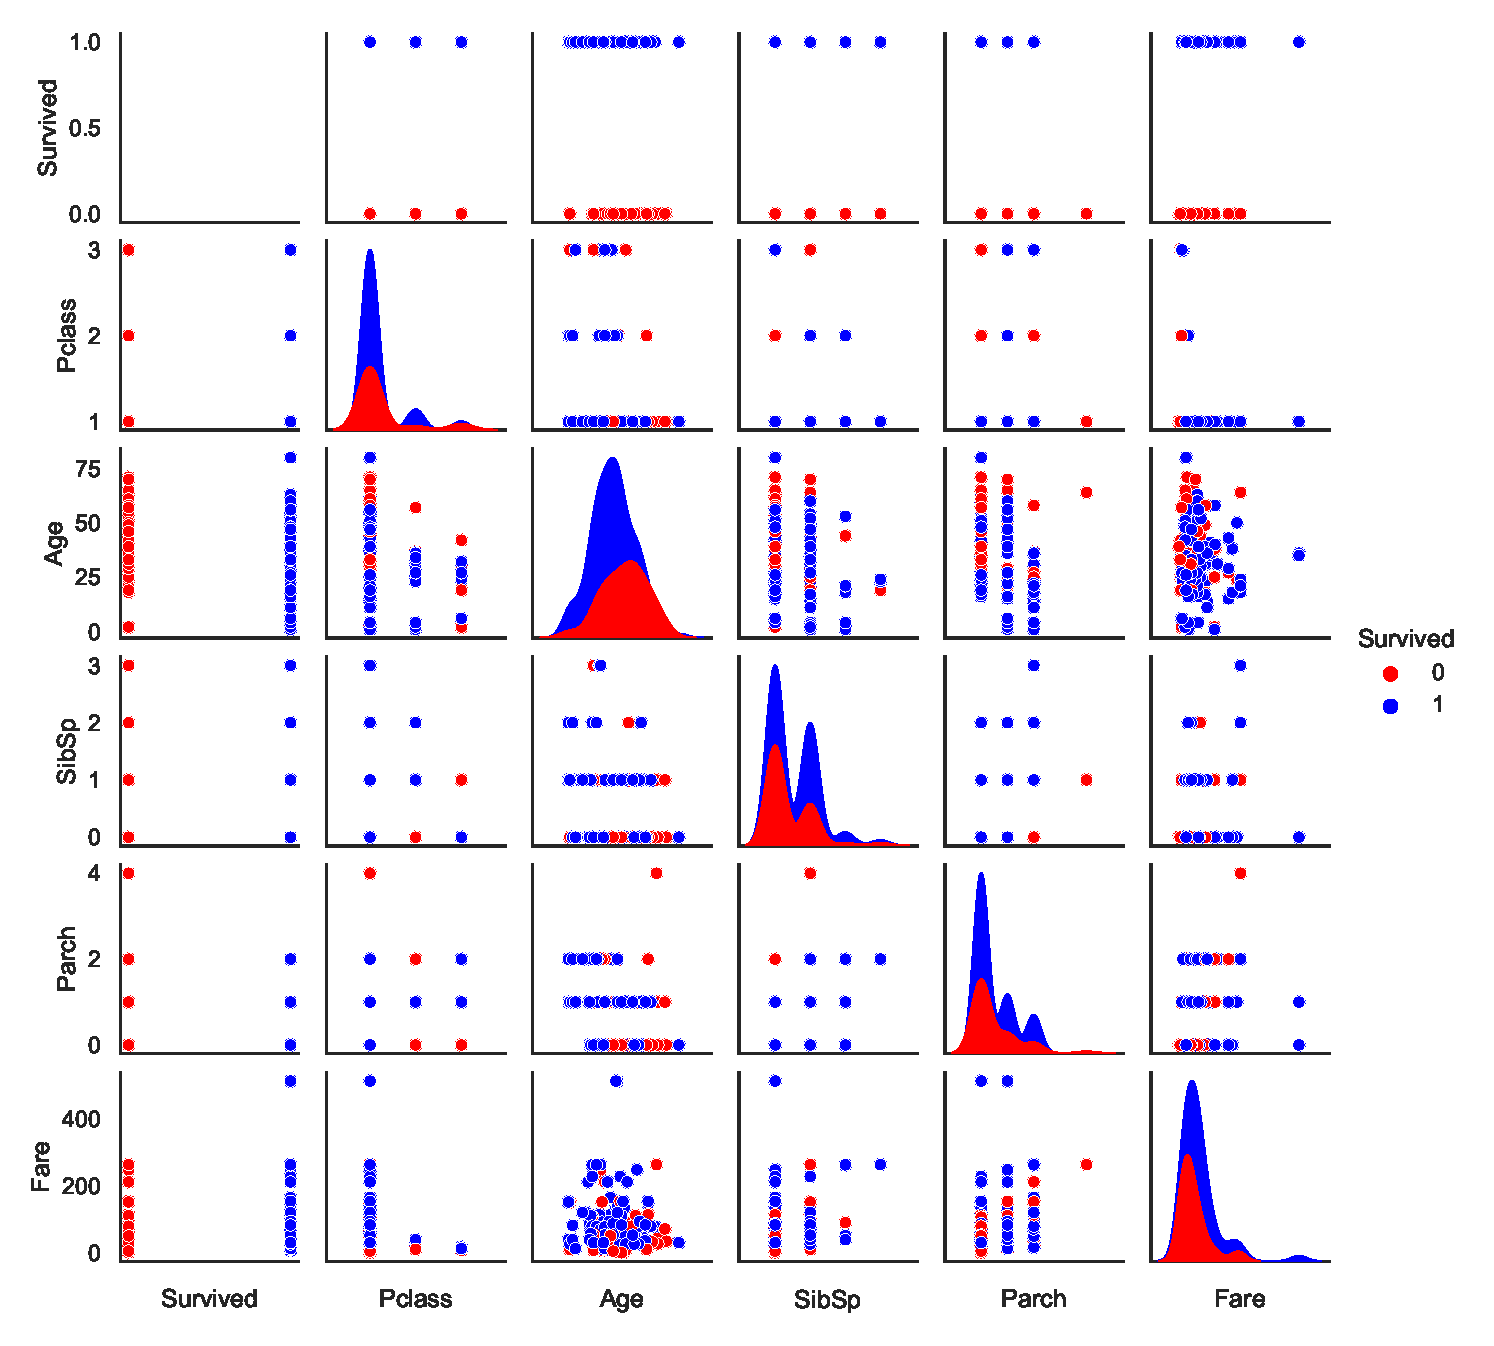
\includegraphics[scale=0.5,width=1.1\textwidth,height=0.4\textwidth]{/Users/pratikshyaparajuli/Desktop/kaggle/KaggleProject/Code/templatex/graphics/titanicimg/relation-between-features.eps}}
  %DIF > \caption{Relation Between The Features}\label{fig:Relation Between Features}
%DIF > \end{figure}
%DIF > \end{slide}
%DIF > %
%%==========================================================================================


%%==========================================================================================
%%
\DIFdelbegin %DIFDELCMD < \begin{slide}[toc=,bm=]{}
%DIFDELCMD < \twocolumn
%DIFDELCMD < {
%DIFDELCMD < %%%
\DIFdel{Group Outlying Aspects Mining
}%DIFDELCMD < \begin{itemize}
%DIFDELCMD < \item
%DIFDELCMD < \smallskip
%DIFDELCMD < %%%
\DIFdel{Focus on differences between \textcolor{orange}{groups}.
}%DIFDELCMD < 

%DIFDELCMD < \item
%DIFDELCMD < \smallskip
%DIFDELCMD < %%%
\DIFdelend \DIFaddbegin \begin{slide}[toc=,bm=]{Correlatoin Matrix}
 \DIFadd{The highest correlation is between }\DIFaddend \textcolor{orange}{\DIFdelbegin \DIFdel{Multiple}\DIFdelend \DIFaddbegin \DIFadd{SibSp and Parch i.e 0.41.}\DIFaddend }
  \DIFdelbegin \DIFdel{points.
}%DIFDELCMD < \medskip
%DIFDELCMD < \end{itemize}
%DIFDELCMD < \vspace{0.75cm}
%DIFDELCMD < %%%
\DIFdelend %\vspace{0.1cm}
  \begin{figure}
    \centering
    \DIFdelbeginFL %DIFDELCMD < \selectcolormodel{rgb}
%DIFDELCMD <   \missingfigure{Testing a long text string.}
%DIFDELCMD <   %%%
%DIF < \includegraphics[width=0.6\textwidth]{figures//example-basketball-projection.eps}\\
  \DIFdelendFL %DIF > \selectcolormodel{rgb}
    \DIFaddbeginFL \centerline{\includegraphics[scale=0.4,width=1.1\textwidth,height=0.5\textwidth]{/Users/pratikshyaparajuli/Desktop/kaggle/KaggleProject/Code/templatex/graphics/titanicimg/heatmap.eps}}
    \DIFaddendFL \caption{\DIFdelbeginFL \DIFdelFL{Group Outlying Aspects Target}\DIFdelendFL \DIFaddbeginFL \DIFaddFL{Interpreting the heatmap}\DIFaddendFL }\DIFdelbeginFL %DIFDELCMD < \label{fig:GroupOutAspect-target}
%DIFDELCMD < %%%
\DIFdelendFL \DIFaddbeginFL \label{fig:Heat map}
  \DIFaddendFL \end{figure}
  \DIFdelbegin %DIFDELCMD < }
%DIFDELCMD < {
%DIFDELCMD < %%%
\DIFdel{Outlying Aspects Mining
}%DIFDELCMD < \begin{itemize}
\begin{itemize}%DIFAUXCMD
%DIFDELCMD < \item
\item%DIFAUXCMD
%DIFDELCMD < %%%
\DIFdel{Concentrates on differences between \textcolor{orange}{objects}.
}%DIFDELCMD < 

%DIFDELCMD < \item
\item%DIFAUXCMD
%DIFDELCMD < %%%
\DIFdel{\textcolor{orange}{One} point.
}
\end{itemize}%DIFAUXCMD
%DIFDELCMD < \end{itemize}
%DIFDELCMD < \bigskip
%DIFDELCMD < \begin{figure}
%DIFDELCMD <   \centering
%DIFDELCMD <   \selectcolormodel{rgb}
%DIFDELCMD <   \missingfigure{Testing a long text string.}
%DIFDELCMD < %%%
%DIF <   \includegraphics[width=0.5\textwidth]{figures//OutAspect_target.eps}\\
  %DIFDELCMD < \caption{%
{%DIFAUXCMD
\DIFdelFL{Outlying Aspects Target}}%DIFAUXCMD
%DIFDELCMD < \label{fig:OutAspect-target}
%DIFDELCMD < \end{figure}
%DIFDELCMD < }
%DIFDELCMD < 

%DIFDELCMD < %%%
%DIF < %==========================================================================================
%DIFDELCMD < \begin{note}
%DIFDELCMD < %%%
\DIFdel{In this research paper,
we proposed the group outlying aspects mining.
Now,
let me summarize the differences between group outlying aspects mining and outlying aspects mining.
}%DIFDELCMD < 

%DIFDELCMD < %%%
\DIFdel{Group outlying aspects mining mainly focuses on the differences between groups.
But outlying aspects mining mainly concentrates on the differences between objects.
The target of group outlying aspects mining can be seen as many points.
While the target of outlying aspects mining can be regarded as one point.
}%DIFDELCMD < 

%DIFDELCMD < %%%
\DIFdel{In the NBA example,
group outlying aspects mining focuses on the advantages
or disadvantages of one team,
however,
outlying aspects mining focuses on the advantages or disadvantages of one player.
}%DIFDELCMD < \end{note}
%DIFDELCMD < %%%
%DIF < %==========================================================================================
%DIFDELCMD < 

%DIFDELCMD < %%%
\DIFdelend \end{slide}
  %%
  %%==========================================================================================

  
  %%==========================================================================================
  %%
\DIFdelbegin %DIFDELCMD < \begin{slide}{Challenges (1)}
%DIFDELCMD < %%%
%DIF < Challenges (1)
%DIFDELCMD < \begin{itemize}
%DIFDELCMD < \item
%DIFDELCMD < %%%
\DIFdel{How to \textcolor{orange}{represent} the group features.
}\DIFdelend %DIF >  \begin{slide}{Finding any relations or trends considering multiple features}
%DIF >  %Challenges (1)
%DIF >  \begin{itemize}
%DIF >  \item
%DIF >  How to \textcolor{orange}{represent} the group features.

\DIFdelbegin %DIFDELCMD < \begin{itemize}
%DIFDELCMD < \item
%DIFDELCMD < %%%
\DIFdel{Can be affected by outlier values.
}\DIFdelend %DIF >  \begin{itemize}
%DIF >  \item
%DIF >  Can be affected by outlier values.

\DIFdelbegin %DIFDELCMD < \item
%DIFDELCMD < %%%
\DIFdel{Can \textcolor{orange}{Not} reflect the overall distribution of group features.
}%DIFDELCMD < \end{itemize}
%DIFDELCMD < \end{itemize}
%DIFDELCMD < %%%
\DIFdelend %DIF >  \item
%DIF >  Can \textcolor{orange}{Not} reflect the overall distribution of group features.
%DIF >  \end{itemize}
%DIF >  \end{itemize}

%DIF < %==========================================================================================
\DIFdelbegin %DIFDELCMD < \begin{note}
%DIFDELCMD < %%%
\DIFdel{Based on current existing methods,
there still remains some research challenges.
}\DIFdelend %DIF >  %%==========================================================================================
%DIF >  % \begin{note}
%DIF >  % Based on current existing methods,
%DIF >  % there still remains some research challenges.

\DIFdelbegin \DIFdel{The first one is how to represent the group features
based on the features of the individuals in the group.
}\DIFdelend %DIF >  % The first one is how to represent the group features
%DIF >  % based on the features of the individuals in the group.

\DIFdelbegin \DIFdel{Although the arithmetic mean of all elements
in each feature can describe the features of one group.
It can be affected by outlier values,
and can't reflect the entire distribution of group features.L
}%DIFDELCMD < \end{note}
%DIFDELCMD < %%%
%DIF < %==========================================================================================
\DIFdelend %DIF >  % Although the arithmetic mean of all elements
%DIF >  % in each feature can describe the features of one group.
%DIF >  % It can be affected by outlier values,
%DIF >  % and can't reflect the entire distribution of group features.L
%DIF >  % \end{note}
%DIF >  %%==========================================================================================

\DIFdelbegin %DIFDELCMD < \end{slide}
%DIFDELCMD < %%%
\DIFdelend %DIF >  \end{slide}
%%
%%==========================================================================================


%%==========================================================================================
%%
\DIFdelbegin %DIFDELCMD < \begin{slide}[toc=,bm=]{Challenges (2)}
%DIFDELCMD < %%%
\DIFdelend %DIF >  \begin{slide}[toc=,bm=]{Challenges (2)}

\DIFdelbegin %DIFDELCMD < \begin{itemize}
%DIFDELCMD < \item
%DIFDELCMD < %%%
\DIFdel{How to \textcolor{orange}{evaluate} the outlying degree in different aspects.
}\DIFdelend %DIF >  \begin{itemize}
%DIF >  \item
%DIF >  How to \textcolor{orange}{evaluate} the outlying degree in different aspects.

\DIFdelbegin %DIFDELCMD < \begin{itemize}
%DIFDELCMD < \item
%DIFDELCMD < %%%
\DIFdel{Need design a scoring function when necessary.
}\DIFdelend %DIF >  \begin{itemize}
%DIF >  \item
%DIF >  Need design a scoring function when necessary.

\DIFdelbegin %DIFDELCMD < \item
%DIFDELCMD < %%%
\DIFdel{Adopting an appropriate scoring function (without dimension bias) remains a problem.
}\DIFdelend %DIF >  \item
%DIF >  Adopting an appropriate scoring function (without dimension bias) remains a problem.

\DIFdelbegin %DIFDELCMD < \end{itemize}
%DIFDELCMD < \end{itemize}
%DIFDELCMD < %%%
\DIFdelend %DIF >  \end{itemize}
%DIF >  \end{itemize}

%DIF < %==========================================================================================
\DIFdelbegin %DIFDELCMD < \begin{note}
%DIFDELCMD < %%%
\DIFdel{The second challenge is how to evaluate the outlying degree of
the query group between different aspects.
}\DIFdelend %DIF >  %%==========================================================================================
%DIF >  \begin{note}
%DIF >  The second challenge is how to evaluate the outlying degree of
%DIF >  the query group between different aspects.

\DIFdelbegin \DIFdel{In that case,
we need to design a scoring function to measure the outlying degree.
But adopting an appropriate scoring function without dimension bias still remains a problem.
}%DIFDELCMD < \end{note}
%DIFDELCMD < %%%
%DIF < %==========================================================================================
\DIFdelend %DIF >  In that case,
%DIF >  we need to design a scoring function to measure the outlying degree.
%DIF >  But adopting an appropriate scoring function without dimension bias still remains a problem.
%DIF >  \end{note}
%DIF >  %%==========================================================================================

\DIFdelbegin %DIFDELCMD < \end{slide}
%DIFDELCMD < %%%
\DIFdelend %DIF >  \end{slide}
%%
%%==========================================================================================
\DIFdelbegin %DIFDELCMD < 

%DIFDELCMD < %%%
\DIFdelend %%==========================================================================================
%%
\DIFdelbegin %DIFDELCMD < \begin{slide}[toc=,bm=]{Challenges (3)}
%DIFDELCMD < %%%
\DIFdelend %DIF >  \begin{slide}[toc=,bm=]{Challenges (3)}

\DIFdelbegin %DIFDELCMD < \begin{itemize}
%DIFDELCMD < \item
%DIFDELCMD < %%%
\DIFdel{How to \textcolor{orange}{improve} the efficiency.
}\DIFdelend %DIF >  \begin{itemize}
%DIF >  \item
%DIF >  How to \textcolor{orange}{improve} the efficiency.

\DIFdelbegin %DIFDELCMD < \begin{itemize}
%DIFDELCMD < %%%
\DIFdelend %DIF >  \begin{itemize}

\DIFdelbegin %DIFDELCMD < \item
%DIFDELCMD < %%%
\DIFdel{When the dimension of the \textcolor{orange}{data is high},
the candidate subspace grows exponentially.
}\DIFdelend %DIF >  \item
%DIF >  When the dimension of the \textcolor{orange}{data is high},
%DIF >  the candidate subspace grows exponentially.

\DIFdelbegin %DIFDELCMD < \item
%DIFDELCMD < %%%
\DIFdel{It will easily go beyond the limits of the computation resources.
}\DIFdelend %DIF >  \item
%DIF >  It will easily go beyond the limits of the computation resources.

\DIFdelbegin %DIFDELCMD < \end{itemize}
%DIFDELCMD < \end{itemize}
%DIFDELCMD < %%%
\DIFdelend %DIF >  \end{itemize}
%DIF >  \end{itemize}

%DIF < %==========================================================================================
\DIFdelbegin %DIFDELCMD < \begin{note}
%DIFDELCMD < %%%
\DIFdel{The third challenge is how to improve efficiency.
}\DIFdelend %DIF >  %%==========================================================================================
%DIF >  \begin{note}
%DIF >  The third challenge is how to improve efficiency.

\DIFdelbegin \DIFdel{To be specific,
when the dimension of data is high,
the candidate subspace increase dramatically,
so that it is very easy to exceed the limit of computer resources.
}%DIFDELCMD < \end{note}
%DIFDELCMD < %%%
%DIF < %==========================================================================================
\DIFdelend %DIF >  To be specific,
%DIF >  when the dimension of data is high,
%DIF >  the candidate subspace increase dramatically,
%DIF >  so that it is very easy to exceed the limit of computer resources.
%DIF >  \end{note}
%DIF >  %%==========================================================================================

\DIFdelbegin %DIFDELCMD < \end{slide}
%DIFDELCMD < %%%
\DIFdelend %DIF >  \end{slide}
%%
%%==========================================================================================


 \section{\DIFdelbegin \DIFdel{GOAM Algorithm}\DIFdelend \DIFaddbegin \DIFadd{Feature Engineering and Data Cleaning}\DIFaddend }


%%==========================================================================================
%%
\DIFdelbegin %DIFDELCMD < \begin{slide}[toc=,bm=]{}
%DIFDELCMD < 

%DIFDELCMD < %%%
\DIFdel{Framework of GOAM algorithm: }%DIFDELCMD < 

%DIFDELCMD < \bigskip
%DIFDELCMD < 

%DIFDELCMD < \begin{figure}
%DIFDELCMD <   \centering
%DIFDELCMD <   \selectcolormodel{rgb}
%DIFDELCMD <   \missingfigure{Testing a long text string.}
%DIFDELCMD < %%%
%DIF <   \includegraphics[width=0.55\textwidth]{figures//framework1.eps}\\
  %DIFDELCMD < \caption{%
{%DIFAUXCMD
\DIFdelFL{Framework of GOAM Algorithm}} %DIFAUXCMD
%DIFDELCMD < \label{framework}
%DIFDELCMD < \end{figure}
%DIFDELCMD < 

%DIFDELCMD < %%%
\DIFdelend \DIFaddbegin \begin{slide}[toc=,bm=]{Converting features into suitable form for modeling}
\begin{itemize}
  \item
   \DIFadd{Age: Age_band
  }\item 
  \DIFadd{Family_size and Alone: Summation of Parch and SibSp
  }\item  
  \DIFadd{Fare: Fare_cat
}\end{itemize}
\smallskip
  \twocolumn[
\savevalue{lfrheight}=7.6cm,
\savevalue{lfrprop}={
linestyle=solid,framearc=.2,linewidth=1pt},
rfrheight=\usevalue{lfrheight},
rfrprop=\usevalue{lfrprop}
]{
  \begin{table}[tb]
    \setlength{\abovecaptionskip}{0pt}
    \setlength{\belowcaptionskip}{10pt}
    %\centering
    \caption{Age_Band}

    \begin{tabular}{p{2.5cm}p{2.9cm}}
    \hline
      Age_band  & Numbers \\
    \hline
       1    & 382 \\
       2    & 325 \\
       0    & 104 \\
       3    & 69  \\
       4    & 11  \\
    \hline
    \end{tabular}
    \end{table}
}{
  \begin{figure}
    \centering
    %\selectcolormodel{rgb}
    \centerline{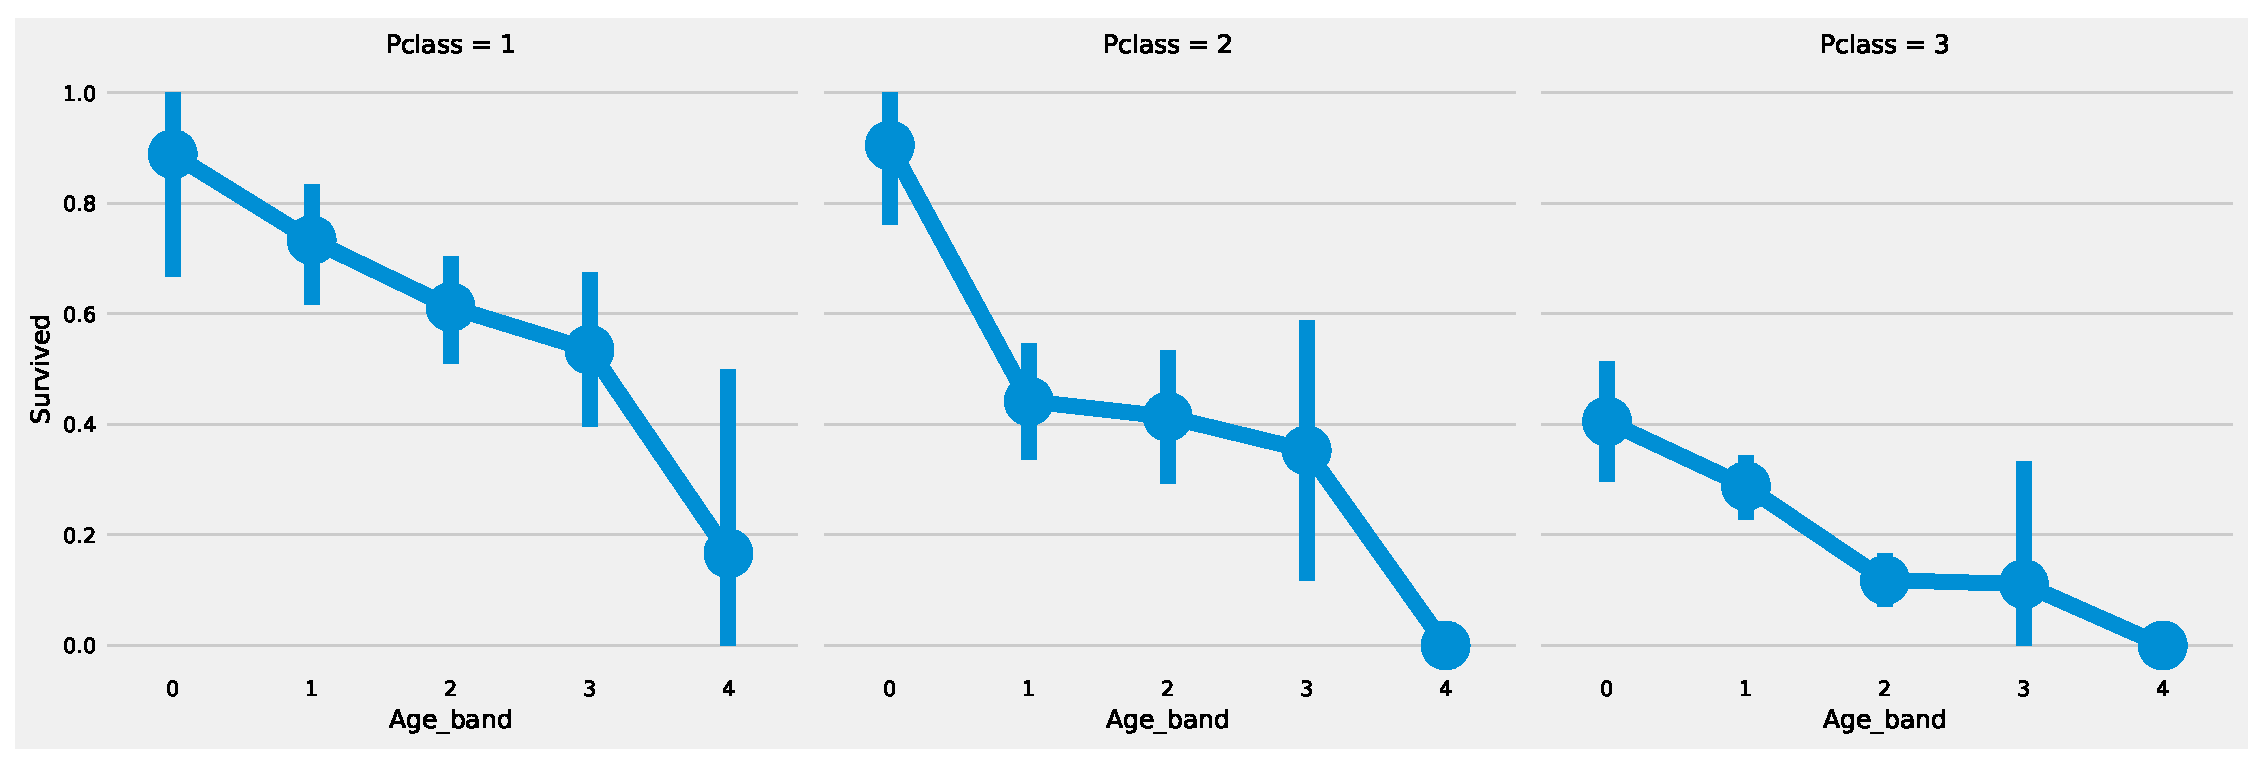
\includegraphics[scale=0.2,width=0.8\textwidth,height=0.5\textwidth]{/Users/pratikshyaparajuli/Desktop/kaggle/KaggleProject/Code/templatex/graphics/titanicimg/age-band.eps}}
    \caption{Age_Band}\label{fig:Age_Band}
  \end{figure}
}
\DIFaddend %%==========================================================================================
\DIFdelbegin %DIFDELCMD < \begin{note}
%DIFDELCMD < %%%
\DIFdel{In order to tackle the above issues,
GOAM algorithm is involved.
}\DIFdelend %DIF >  \begin{note}
%DIF >  In order to tackle the above issues,
%DIF >  GOAM algorithm is involved.

\DIFdelbegin \DIFdel{Let's have a look at the framework of this algorithm.
The first step is to use the histogram to represent the group features
based on all individuals in the group.
}\DIFdelend %DIF >  Let's have a look at the framework of this algorithm.
%DIF >  The first step is to use the histogram to represent the group features
%DIF >  based on all individuals in the group.

\DIFdelbegin \DIFdel{Following that,
we utilize the earth mover distances to measure the
outlying degree between groups.
This is the second step:
outlying degree scoring.
}\DIFdelend %DIF >  Following that,
%DIF >  we utilize the earth mover distances to measure the
%DIF >  outlying degree between groups.
%DIF >  This is the second step:
%DIF >  outlying degree scoring.

\DIFdelbegin \DIFdel{The last step is to identify the outlying aspects.
}\DIFdelend %DIF >  The last step is to identify the outlying aspects.

\DIFdelbegin %DIFDELCMD < \end{note}
%DIFDELCMD < %%%
\DIFdelend %DIF >  \end{note}
%%==========================================================================================

\end{slide}
%%
%%==========================================================================================


%%==========================================================================================
%%
\DIFdelbegin %DIFDELCMD < \begin{slide}{Step One - Group Feature Extraction}
%DIFDELCMD < %%%
\DIFdelend \DIFaddbegin \begin{slide}{Removing Redundant features}
\DIFaddend %Step One - Group Feature Extraction}
\begin{itemize}
\item
  \DIFdelbegin %DIFDELCMD < \smallskip
%DIFDELCMD < %%%
\DIFdel{Suppose $f_1$, $f_2$, $f_3$ are three features of $G_q$}\DIFdelend \DIFaddbegin \DIFadd{Name--> We don't need name feature as it cannot be converted into any categorical value.
  }\item
  \DIFadd{Ticket--> It is any random string that cannot be categorised.
  }\item
  \DIFadd{Fare--> We have the Fare_cat feature, so unneeded
  }\item
   \DIFadd{Cabin--> A lot of NaN values and also many passengers have multiple cabins. So this is a useless feature.
  }\item
   \DIFadd{Fare_Range--> We have the fare_cat feature}\DIFaddend .
  \DIFdelbegin %DIFDELCMD < 

%DIFDELCMD < %%%
\DIFdel{$f_1$: \{$x_1, x_2, x_3, x_4, x_5, x_2, x_3, x_4, x_1, x_2$\} }%DIFDELCMD < \\
%DIFDELCMD < 

%DIFDELCMD < %%%
\DIFdel{$f_2$: \{$y_2, y_2, y_1, y_2, y_3, y_3, y_5, y_4, y_4, y_2$\} }%DIFDELCMD < \\
%DIFDELCMD < 

%DIFDELCMD < %%%
\DIFdel{$f_3$: \{$z_1, z_4, z_2, z_4, z_5, z_3, z_1, z_2, z_4, z_2$\} }%DIFDELCMD < \\
%DIFDELCMD < %%%
\DIFdelend \DIFaddbegin \item
  \DIFadd{PassengerId--> Cannot be categorised.
}\DIFaddend \end{itemize}
\DIFdelbegin %DIFDELCMD < 

%DIFDELCMD < \begin{figure}[htbp]
%DIFDELCMD <     \centering
%DIFDELCMD <     \subfigure[$f_1$]{
%DIFDELCMD <         \selectcolormodel{rgb}
%DIFDELCMD <         \missingfigure[figwidth=5.5cm]{Test.}
%DIFDELCMD <         %\includegraphics[width=0.25\textwidth]{figures//frequency-distribution-feature1.eps}
%DIFDELCMD <         \label{fig:fre-dis-f1}
%DIFDELCMD <     }
%DIFDELCMD <     \subfigure[$f_2$]{
%DIFDELCMD <         \selectcolormodel{rgb}
%DIFDELCMD <         \missingfigure[figwidth=5.5cm]{Test.}
%DIFDELCMD <         \label{fig:fre-dis-f2}
%DIFDELCMD <     }
%DIFDELCMD <     \subfigure[$f_3$]{
%DIFDELCMD <         \selectcolormodel{rgb}
%DIFDELCMD <         \missingfigure[figwidth=5.5cm]{Test.}
%DIFDELCMD <         \label{fig:fre-dis-f3}
%DIFDELCMD <     }
%DIFDELCMD <     %%%
%DIFDELCMD < \caption{%
{%DIFAUXCMD
\DIFdelFL{Histogram of $G_q$ on three features}}
    %DIFAUXCMD
%DIFDELCMD < \label{fig:fre-dis-each-feature}
%DIFDELCMD < \end{figure}
%DIFDELCMD < 

%DIFDELCMD < %%%
%DIF < %==========================================================================================
%DIFDELCMD < \begin{note}
%DIFDELCMD < %%%
\DIFdel{Now, let me specifically explain what each step means.
The first step is group feature extraction.
we can take one group extraction as an example.
  }%DIFDELCMD < 

%DIFDELCMD < %%%
\DIFdel{We suppose to use $f_1$, $f_2$, $f_3$ to represent three features of $G_q$.
The values of $f_1$ are }%DIFDELCMD < {%%%
\DIFdel{$x_1$, $x_2$, $x_3$, $x_4$}%DIFDELCMD < } %%%
\DIFdel{and so on. And the values of $f_2$ are }%DIFDELCMD < {%%%
\DIFdel{$y_2$, $y_2$, $y_1$, $x_2$}%DIFDELCMD < } %%%
\DIFdel{and so on.
}%DIFDELCMD < 

%DIFDELCMD < %%%
\DIFdel{For feature $f_1$,
we use the histogram to illustrate feature $f_1$ after
counting the frequency of each value,
as show in figure 6 (a ).
  }%DIFDELCMD < 

%DIFDELCMD < %%%
\DIFdel{Similarly,
we can also extract other features of the group
according to feature$f_1$.
  }%DIFDELCMD < \end{note}
%DIFDELCMD < %%%
%DIF < %==========================================================================================
%DIFDELCMD < 

%DIFDELCMD < %%%
\DIFdelend \end{slide}
%%
%%==========================================================================================
\DIFdelbegin %DIFDELCMD < 

%DIFDELCMD < %%%
%DIF < %==========================================================================================
%DIF < %
%DIFDELCMD < \begin{slide}{Step Two - Outlying Degree Scoring}
%DIFDELCMD < %%%
%DIF < Step Two - Outlying Degree Scoring
%DIFDELCMD < \begin{itemize}
\begin{itemize}%DIFAUXCMD
%DIFDELCMD < \item
\item%DIFAUXCMD
%DIFDELCMD < %%%
\DIFdel{Calculate Earth Mover Distance
}%DIFDELCMD < 

%DIFDELCMD < \begin{itemize}
%DIFDELCMD < \item
\item%DIFAUXCMD
%DIFDELCMD < %%%
\DIFdel{Represent one feature among different groups
}%DIFDELCMD < 

%DIFDELCMD < \item
\item%DIFAUXCMD
%DIFDELCMD < %%%
\DIFdel{Purpose: calculate the minimum mean distance
}
\end{itemize}%DIFAUXCMD
%DIFDELCMD < \end{itemize}
%DIFDELCMD < 

%DIFDELCMD < %%%
\DIFdelend \DIFaddbegin \begin{slide}{Correlation Matrix after Data Cleaning}
  \DIFadd{Positive correlation: \textcolor{orange}{SibSp andd Family_Size and Parch and Family_Size} and Negative correlation: \textcolor{orange}{Alone and Family_Size}
   %DIF > \vspace{0.1cm}
   }\DIFaddend \begin{figure}
     \DIFdelbeginFL %DIFDELCMD < \selectcolormodel{rgb}
%DIFDELCMD <    \missingfigure{Make a sketch of the structure of a trebuchet.}
%DIFDELCMD < %%%
%DIF <   \includegraphics[width=0.4\textwidth]{figures//example3.eps}\\
   \DIFdelendFL \DIFaddbeginFL \centering
     %DIF > \selectcolormodel{rgb}
     \centerline{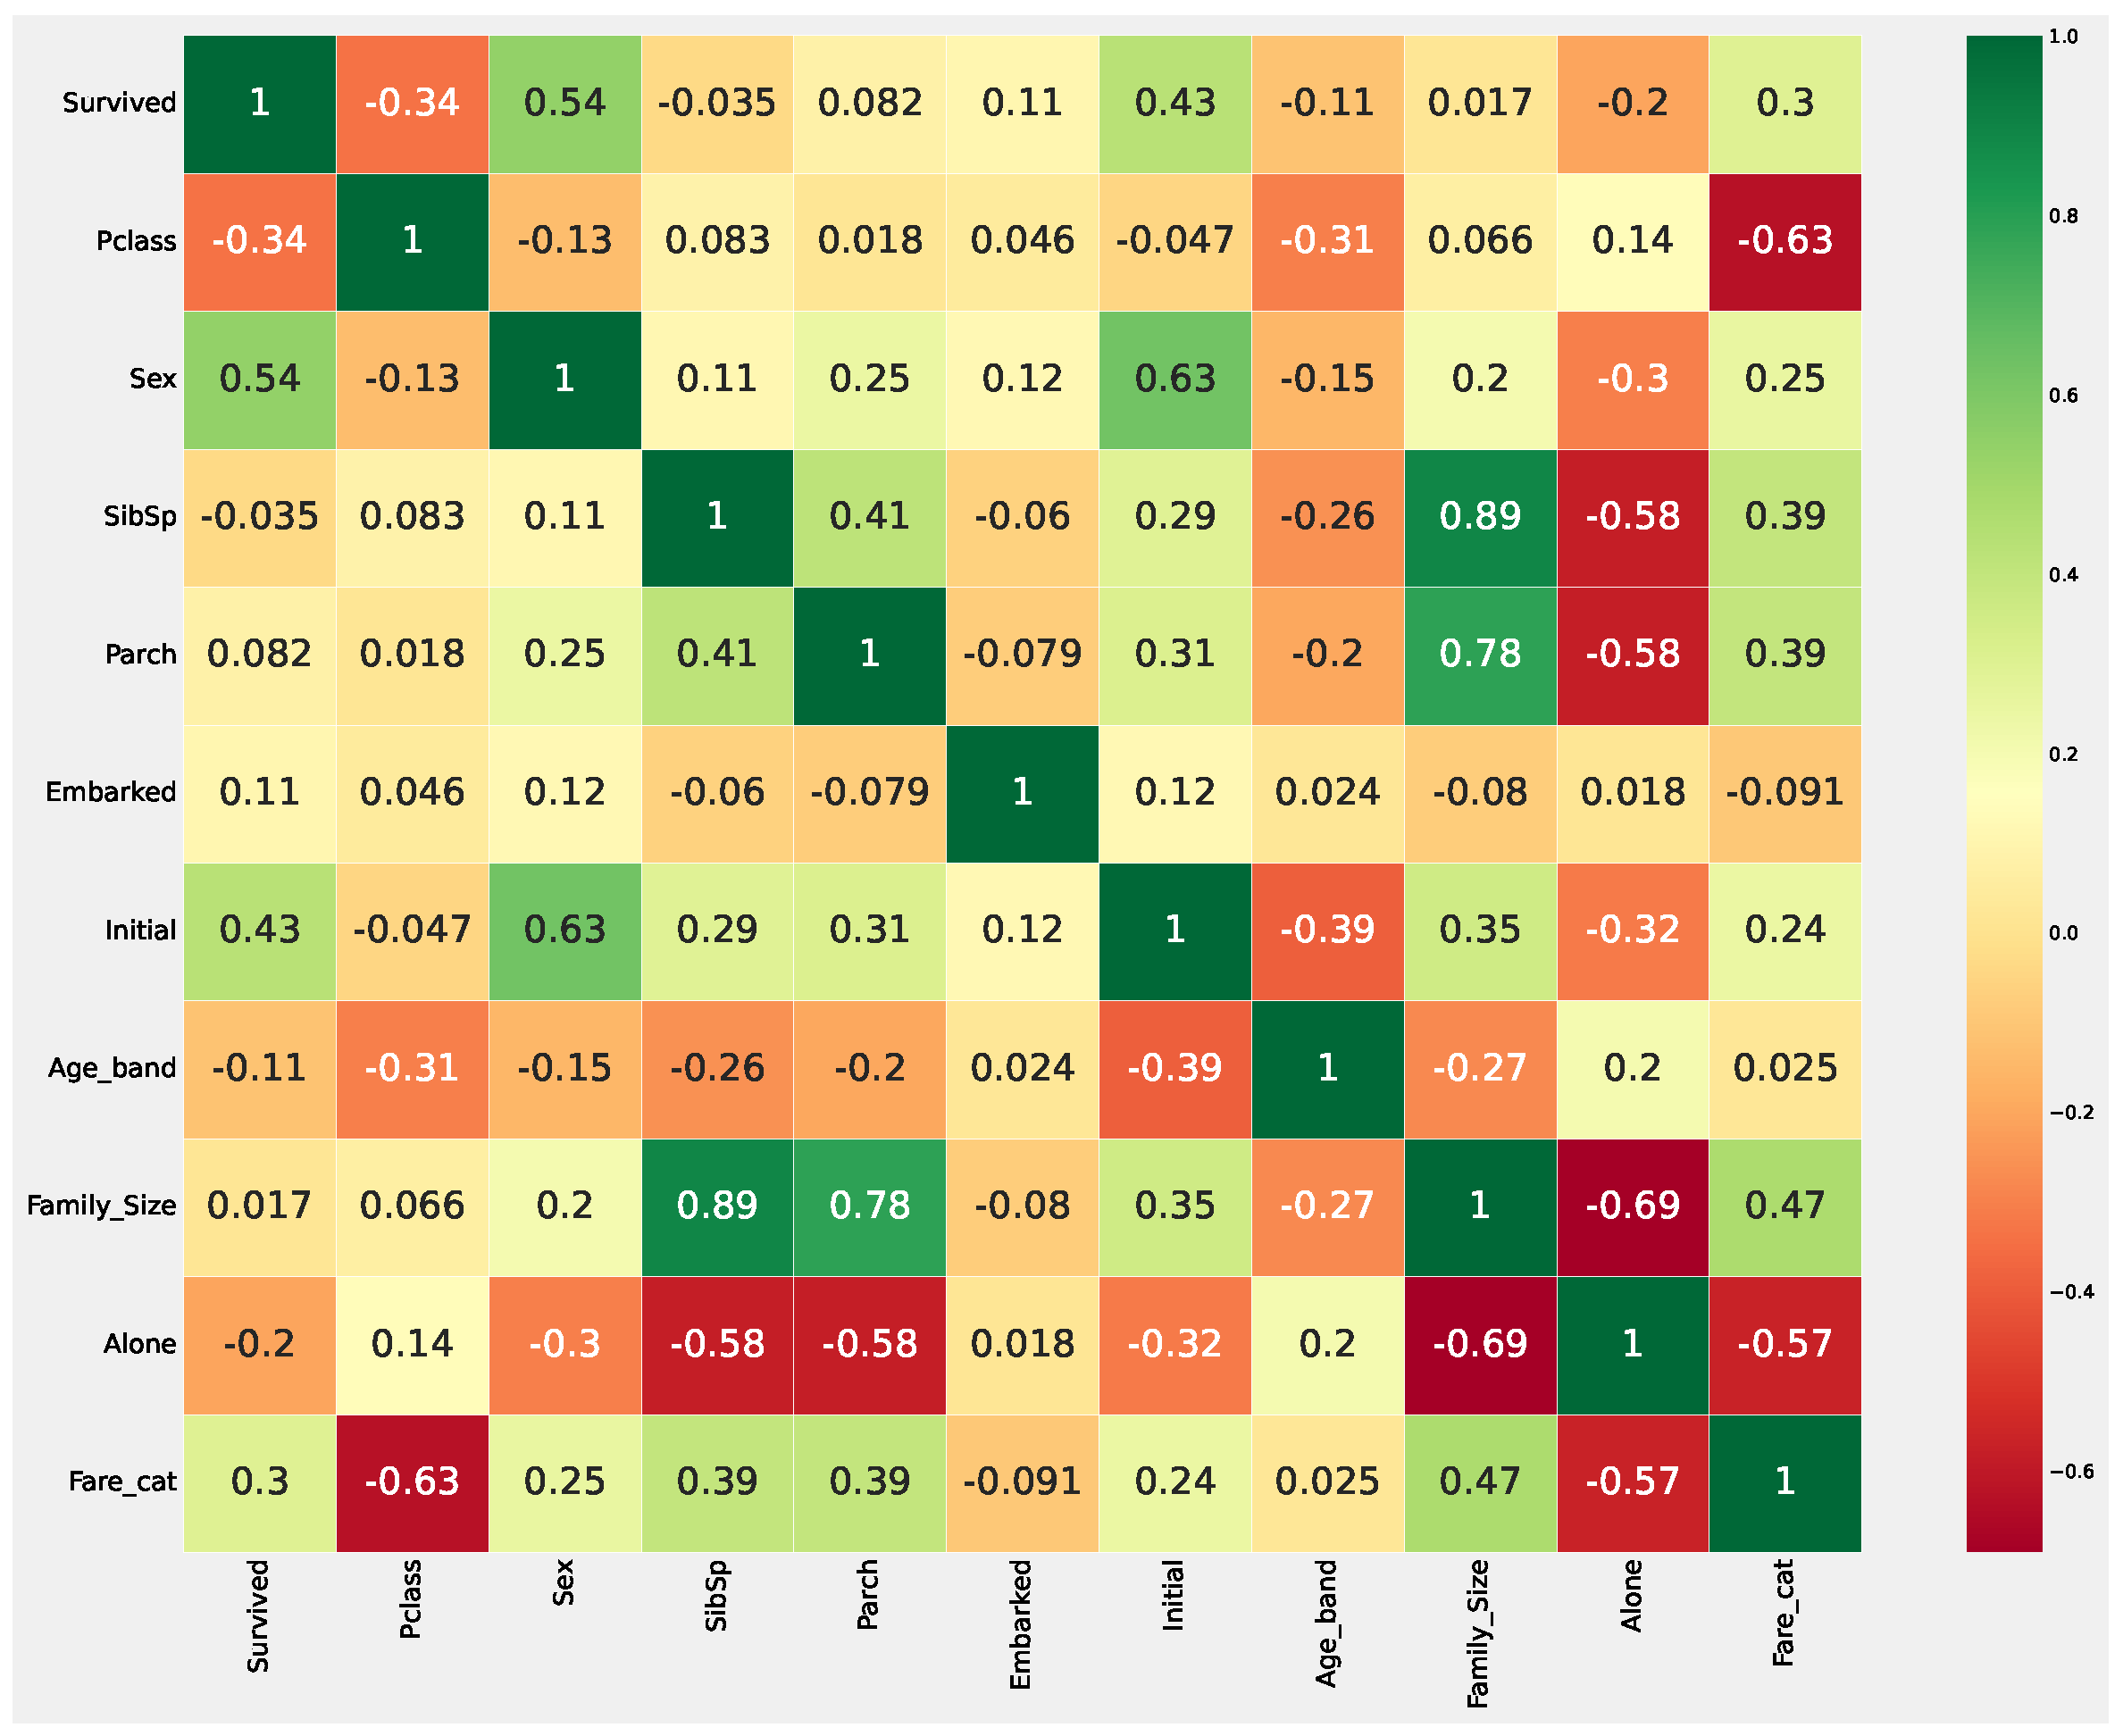
\includegraphics[scale=0.4,width=1.1\textwidth,height=0.45\textwidth]{/Users/pratikshyaparajuli/Desktop/kaggle/KaggleProject/Code/templatex/graphics/titanicimg/clean-heatmap.eps}}
     \DIFaddendFL \caption{\DIFdelbeginFL \DIFdelFL{EMD of one feature}\DIFdelendFL \DIFaddbeginFL \DIFaddFL{Correlation Matrix after Data Cleaning}\DIFaddendFL }\DIFdelbeginFL %DIFDELCMD < \label{EMD}
%DIFDELCMD < %%%
\DIFdelendFL \DIFaddbeginFL \label{fig:clean-Heat map}
   \DIFaddendFL \end{figure}
   \DIFdelbegin %DIFDELCMD < \end{itemize}
%DIFDELCMD < %%%
\DIFdelend \DIFaddbegin \end{slide}
\DIFaddend 

%DIF < %==========================================================================================
\DIFdelbegin %DIFDELCMD < \begin{note}
%DIFDELCMD < %%%
\DIFdel{The second step is outlying degree scoring,
which is to evaluate the outlying degree between the target group and competitive groups.
}\DIFdelend \DIFaddbegin \section{\DIFadd{Predictive Modeling}}
\DIFaddend 


\DIFdelbegin \DIFdel{First,
we calculate the earth mover distance of one feature in different groups.
}%DIFDELCMD < 

%DIFDELCMD < %%%
\DIFdel{The earth mover distance reflects the minimum mean distance between
the target group and other groups on one feature.
}%DIFDELCMD < 

%DIFDELCMD < %%%
\DIFdel{Later on,
we utilize the EMD to measure the differences between groups.
}%DIFDELCMD < \end{note}
%DIFDELCMD < %%%
\DIFdelend %%==========================================================================================
\DIFdelbegin %DIFDELCMD < 

%DIFDELCMD < \end{slide}
%DIFDELCMD < %%%
\DIFdelend %%
%DIF < %==========================================================================================
\DIFaddbegin \begin{slide}[toc=,bm=]{Evaluation Classification Algorithms}
\DIFaddend 

%DIF < %==========================================================================================
%DIF < %
\DIFdelbegin %DIFDELCMD < \begin{slide}[toc=,bm=]{Step Two - Outlying Degree Scoring}
%DIFDELCMD < 

%DIFDELCMD < %%%
\DIFdelend \DIFaddbegin \begin{center}
\DIFaddend \begin{itemize}
\item
\DIFdelbegin \DIFdel{Calculate the outlying degree
}%DIFDELCMD < 

%DIFDELCMD < \vspace{1.2cm}
%DIFDELCMD < 

%DIFDELCMD < \begin{centering}
%DIFDELCMD < 

%DIFDELCMD < %%%
\DIFdel{$ OD(G_q) = \sum_{1}^{n}EDM(h_{q_s}, h_{k_s}) $
}%DIFDELCMD < 

%DIFDELCMD < \end{centering}
%DIFDELCMD < 

%DIFDELCMD < \begin{itemize}
%DIFDELCMD < %%%
\DIFdelend \DIFaddbegin \DIFadd{Logistic Regression
}\DIFaddend \item
\DIFdelbegin \DIFdel{n $\Leftrightarrow$ the number of contrast groups.
}%DIFDELCMD < 

%DIFDELCMD < %%%
\DIFdelend \DIFaddbegin \DIFadd{Support Vector Machines (Linear and radial)
}\DIFaddend \item
\DIFdelbegin \DIFdel{$h_{k_s}$  $\Leftrightarrow$ the histogram representation of $G_k$ in the subspace s.
}%DIFDELCMD < 

%DIFDELCMD < \end{itemize}
%DIFDELCMD < \end{itemize}
%DIFDELCMD < 

%DIFDELCMD < %%%
%DIF < %==========================================================================================
%DIFDELCMD < \begin{note}
%DIFDELCMD < %%%
\DIFdel{Base on the earth mover distance,
we can calculate the outlying degree using the formula shown on the screen.
}%DIFDELCMD < 

%DIFDELCMD < %%%
\DIFdel{This formula is the outlying degree scoring function,
n represents the number of competitive groups.
$h_{k_s}$ is the histogram of $G_k$ in the subspace s.
}%DIFDELCMD < \end{note}
%DIFDELCMD < %%%
%DIF < %==========================================================================================
%DIFDELCMD < 

%DIFDELCMD < \end{slide}
%DIFDELCMD < %%%
%DIF < %
%DIF < %==========================================================================================
%DIFDELCMD < 

%DIFDELCMD < %%%
%DIF < %==========================================================================================
%DIF < %
%DIFDELCMD < \begin{slide}{Step Three - Outlying Aspects Identification}
%DIFDELCMD < %%%
%DIF < Step Three - Outlying Aspects Identification
%DIFDELCMD < \begin{itemize}
%DIFDELCMD < %%%
\DIFdelend \DIFaddbegin \DIFadd{Random Forest
}\DIFaddend \item
\DIFdelbegin \DIFdel{Identify group outlying aspects mining based on the value
of outlying degree.
}%DIFDELCMD < 

%DIFDELCMD < %%%
\DIFdelend \DIFaddbegin \DIFadd{K-Nearest Neighbours
}\DIFaddend \item
\DIFdelbegin \DIFdel{The greater the outlying degree is,
the more likely it is group outlying aspect.
}\DIFdelend \DIFaddbegin \DIFadd{Naive Bayes
}\item
\DIFadd{Decision Tree
}\DIFaddend \end{itemize}
\DIFaddbegin \end{center}
\DIFaddend 

%%==========================================================================================
\DIFdelbegin %DIFDELCMD < \begin{note}
%DIFDELCMD < %%%
\DIFdel{Next,
let me talk about the third step.
}\DIFdelend %DIF >  \begin{note}
%DIF >  Before showing the experiment results,
%DIF >  I will introduce the evaluation of the experiment.

\DIFdelbegin \DIFdel{In this step,
we identify the group outlying aspects according to the value of the outlying degree.
}%DIFDELCMD < 

%DIFDELCMD < %%%
\DIFdel{If a feature's outlying degree is greater,
it is more likely to be a group outlying aspect.
}%DIFDELCMD < \end{note}
%DIFDELCMD < %%%
\DIFdelend %DIF >  We use accuracy formula to make comparisons between GOAM algorithm
%DIF >  and outlying aspect mining method.
%DIF >  In the accuracy formula,
%DIF >  P stands for identified outlying aspects;
%DIF >  and T means the real outlying aspects.
%DIF >  \end{note}
%%==========================================================================================

\end{slide}
%%
%%==========================================================================================


%%==========================================================================================
%%
\DIFdelbegin %DIFDELCMD < \begin{slide}[toc=,bm=]{Pseudo code}
%DIFDELCMD < %%%
\DIFdelend \DIFaddbegin \begin{slide}{Prediction Accuracy}
\DIFaddend 

\begin{itemize}
\item 
   \DIFdelbegin \DIFdel{Pseudo code of GOAM algorithm
}%DIFDELCMD < 

%DIFDELCMD < %%%
\DIFdelend \DIFaddbegin \DIFadd{Split the train sample into train and test dataset
   }\item 
   \DIFadd{Train Data_size : 0.7 and Test Data_size : 0.3
   }\item 
   \DIFadd{Total sample size = 891; training sample size = 623, testing sample size = 268
  }\DIFaddend \end{itemize}

\DIFdelbegin %DIFDELCMD < \begin{figure}
%DIFDELCMD <   \centering
%DIFDELCMD <   \selectcolormodel{rgb}
%DIFDELCMD <   \missingfigure[figwidth=16cm]{Testing a long text string}
%DIFDELCMD <   %%%
%DIF < \includegraphics[width=0.75\textwidth]{figures//GOAM.eps}\\
  %DIF < \caption{GOAM Algorithm}\label{OS-Identification}
%DIFDELCMD < \end{figure}
%DIFDELCMD < 

%DIFDELCMD < %%%
%DIF < %==========================================================================================
%DIFDELCMD < \begin{note}
%DIFDELCMD < %%%
\DIFdel{Last,
we use the outlying degree to identify the specific group outlying aspects.
}%DIFDELCMD < 

%DIFDELCMD < %%%
\DIFdel{The pseudo code of GOAM algorithm is as follows.
The input is the group data, the output is outlying aspects of specific group ($G_1$).
}%DIFDELCMD < 

%DIFDELCMD < %%%
\DIFdel{The details of the algorithm I will use an example to explain.
}%DIFDELCMD < \end{note}
%DIFDELCMD < 

%DIFDELCMD < %%%
%DIF < %==========================================================================================
%DIFDELCMD < \end{slide}
%DIFDELCMD < %%%
%DIF < %
%DIF < %==========================================================================================
%DIFDELCMD < 

%DIFDELCMD < %%%
%DIF < %==========================================================================================
%DIF < %
%DIFDELCMD < \begin{slide}[toc=,bm=]{Illustration}
%DIFDELCMD < %%%
%DIF <  Outlying Aspects Identification
\DIFdelend \begin{table}
\setlength{\abovecaptionskip}{0pt}
\setlength{\belowcaptionskip}{10pt}
\centering
\caption{\DIFdelbeginFL \DIFdelFL{Original Dataset}\DIFdelendFL \DIFaddbeginFL \DIFaddFL{Accuracy Comparison of different Classifier Algorithms}\DIFaddendFL }
\DIFdelbeginFL %DIFDELCMD < \begin{tabular}{ccccc | ccccc}
%DIFDELCMD <   %%%
\DIFdelendFL \DIFaddbeginFL 

\begin{tabular}{cccc}
  \DIFaddendFL \toprule
  \DIFdelbeginFL \DIFdelFL{$G_1$ }\DIFdelendFL %DIF >  after \\: \hline or \cline{col1-col2} \cline{col3-col4} ...
   & \DIFdelbeginFL \DIFdelFL{$F_1$ }%DIFDELCMD < & %%%
\DIFdelFL{$F_2$ }%DIFDELCMD < & %%%
\DIFdelFL{$F_3$ }%DIFDELCMD < & %%%
\DIFdelFL{$F_4$ }%DIFDELCMD < & %%%
\DIFdelFL{$G_2$ }%DIFDELCMD < & %%%
\DIFdelFL{$F_1$ }%DIFDELCMD < & %%%
\DIFdelFL{$F_2$ }%DIFDELCMD < & %%%
\DIFdelFL{$F_3$ }%DIFDELCMD < & %%%
\DIFdelFL{$F_4$ }\DIFdelendFL \DIFaddbeginFL \DIFaddFL{Acuracy }\DIFaddendFL \\
\midrule
  \DIFaddbeginFL \DIFaddFL{Radial Support Vector Machines(rbf-SVM)   }\DIFaddendFL & \DIFdelbeginFL \DIFdelFL{10 }%DIFDELCMD < & %%%
\DIFdelFL{8 }%DIFDELCMD < & %%%
\DIFdelFL{9 }%DIFDELCMD < & %%%
\DIFdelFL{8 }%DIFDELCMD < & &%%%
\DIFdelFL{7 }%DIFDELCMD < & %%%
\DIFdelFL{7 }%DIFDELCMD < & %%%
\DIFdelFL{6 }%DIFDELCMD < & %%%
\DIFdelFL{6 }\DIFdelendFL \DIFaddbeginFL \DIFaddFL{0.835820895522388 }\DIFaddendFL \\
  \DIFaddbeginFL \DIFaddFL{Linear Support Vector Machine(linear-SVM) }\DIFaddendFL & \DIFdelbeginFL \DIFdelFL{9  }%DIFDELCMD < & %%%
\DIFdelFL{9 }%DIFDELCMD < & %%%
\DIFdelFL{7 }%DIFDELCMD < & %%%
\DIFdelFL{9 }%DIFDELCMD < & &%%%
\DIFdelFL{8 }%DIFDELCMD < & %%%
\DIFdelFL{9 }%DIFDELCMD < & %%%
\DIFdelFL{9 }%DIFDELCMD < & %%%
\DIFdelFL{8 }\DIFdelendFL \DIFaddbeginFL \DIFaddFL{0.8171641791044776 }\DIFaddendFL \\
  \DIFaddbeginFL \DIFaddFL{Logistic Regression }\DIFaddendFL & \DIFdelbeginFL \DIFdelFL{8  }%DIFDELCMD < & %%%
\DIFdelFL{10}%DIFDELCMD < & %%%
\DIFdelFL{8 }%DIFDELCMD < & %%%
\DIFdelFL{8 }%DIFDELCMD < & &%%%
\DIFdelFL{6 }%DIFDELCMD < & %%%
\DIFdelFL{7 }%DIFDELCMD < & %%%
\DIFdelFL{8 }%DIFDELCMD < & %%%
\DIFdelFL{9  }\DIFdelendFL \DIFaddbeginFL \DIFaddFL{0.8134328358208955 }\DIFaddendFL \\
  \DIFaddbeginFL \DIFaddFL{Decision Tree }\DIFaddendFL & \DIFdelbeginFL \DIFdelFL{8  }%DIFDELCMD < & %%%
\DIFdelFL{8 }%DIFDELCMD < & %%%
\DIFdelFL{6 }%DIFDELCMD < & %%%
\DIFdelFL{7 }%DIFDELCMD < & &%%%
\DIFdelFL{7 }%DIFDELCMD < & %%%
\DIFdelFL{7 }%DIFDELCMD < & %%%
\DIFdelFL{7 }%DIFDELCMD < & %%%
\DIFdelFL{8  }\DIFdelendFL \DIFaddbeginFL \DIFaddFL{0.8059701492537313 }\DIFaddendFL \\
  \DIFaddbeginFL \DIFaddFL{K-Nearest Neighbours(KNN) }\DIFaddendFL & \DIFdelbeginFL \DIFdelFL{9  }%DIFDELCMD < & %%%
\DIFdelFL{9 }%DIFDELCMD < & %%%
\DIFdelFL{9 }%DIFDELCMD < & %%%
\DIFdelFL{8 }%DIFDELCMD < & &%%%
\DIFdelFL{8 }%DIFDELCMD < & %%%
\DIFdelFL{6 }%DIFDELCMD < & %%%
\DIFdelFL{6 }%DIFDELCMD < & %%%
\DIFdelFL{7  }\DIFdelendFL \DIFaddbeginFL \DIFaddFL{0.832089552238806 }\DIFaddendFL \\
  \DIFdelbeginFL %DIFDELCMD < \midrule
%DIFDELCMD <    %%%
\DIFdelFL{$G_3$ }\DIFdelendFL \DIFaddbeginFL \DIFaddFL{Gaussian Naive Bayes }\DIFaddendFL & \DIFdelbeginFL \DIFdelFL{$F_1$ }%DIFDELCMD < & %%%
\DIFdelFL{$F_2$ }%DIFDELCMD < & %%%
\DIFdelFL{$F_3$ }%DIFDELCMD < & %%%
\DIFdelFL{$F_4$ }%DIFDELCMD < & %%%
\DIFdelFL{$G_4$ }%DIFDELCMD < & %%%
\DIFdelFL{$F_1$ }%DIFDELCMD < & %%%
\DIFdelFL{$F_2$ }%DIFDELCMD < & %%%
\DIFdelFL{$F_3$ }%DIFDELCMD < & %%%
\DIFdelFL{$F_4$ }\DIFdelendFL \DIFaddbeginFL \DIFaddFL{0.8134328358208955 }\DIFaddendFL \\
  \DIFdelbeginFL %DIFDELCMD < \midrule
%DIFDELCMD <    %%%
\DIFdelendFL \DIFaddbeginFL \DIFaddFL{Random Forests }\DIFaddendFL & \DIFdelbeginFL \DIFdelFL{8 }%DIFDELCMD < & %%%
\DIFdelFL{10 }%DIFDELCMD < & %%%
\DIFdelFL{8 }%DIFDELCMD < & %%%
\DIFdelFL{8 }%DIFDELCMD < & &%%%
\DIFdelFL{9 }%DIFDELCMD < & %%%
\DIFdelFL{8 }%DIFDELCMD < & %%%
\DIFdelFL{8 }%DIFDELCMD < & %%%
\DIFdelFL{8}\DIFdelendFL \DIFaddbeginFL \DIFaddFL{0.8208955223880597}\DIFaddendFL \\
\DIFdelbeginFL %DIFDELCMD < &%%%
\DIFdelFL{9 }%DIFDELCMD < & %%%
\DIFdelFL{9  }%DIFDELCMD < & %%%
\DIFdelFL{7 }%DIFDELCMD < & %%%
\DIFdelFL{9 }%DIFDELCMD < & &%%%
\DIFdelFL{7 }%DIFDELCMD < & %%%
\DIFdelFL{7 }%DIFDELCMD < & %%%
\DIFdelFL{7 }%DIFDELCMD < & %%%
\DIFdelFL{9}%DIFDELCMD < \\
%DIFDELCMD <    &%%%
\DIFdelFL{10}%DIFDELCMD < & %%%
\DIFdelFL{9  }%DIFDELCMD < & %%%
\DIFdelFL{10}%DIFDELCMD < & %%%
\DIFdelFL{7 }%DIFDELCMD < & &%%%
\DIFdelFL{8 }%DIFDELCMD < & %%%
\DIFdelFL{6 }%DIFDELCMD < & %%%
\DIFdelFL{6 }%DIFDELCMD < & %%%
\DIFdelFL{8}%DIFDELCMD < \\
%DIFDELCMD <    &%%%
\DIFdelFL{9 }%DIFDELCMD < & %%%
\DIFdelFL{10 }%DIFDELCMD < & %%%
\DIFdelFL{8 }%DIFDELCMD < & %%%
\DIFdelFL{6 }%DIFDELCMD < & &%%%
\DIFdelFL{9 }%DIFDELCMD < & %%%
\DIFdelFL{8 }%DIFDELCMD < & %%%
\DIFdelFL{8 }%DIFDELCMD < & %%%
\DIFdelFL{7}%DIFDELCMD < \\
%DIFDELCMD <    &%%%
\DIFdelFL{9 }%DIFDELCMD < & %%%
\DIFdelFL{9  }%DIFDELCMD < & %%%
\DIFdelFL{7 }%DIFDELCMD < & %%%
\DIFdelFL{9 }%DIFDELCMD < & &%%%
\DIFdelFL{8 }%DIFDELCMD < & %%%
\DIFdelFL{7 }%DIFDELCMD < & %%%
\DIFdelFL{9 }%DIFDELCMD < & %%%
\DIFdelFL{8}%DIFDELCMD < \\
%DIFDELCMD <   %%%
\DIFdelendFL \bottomrule
\end{tabular}
\end{table}

%DIF < %==========================================================================================
\DIFdelbegin %DIFDELCMD < \begin{note}
%DIFDELCMD < %%%
\DIFdel{Next,
let me use an example to explain GOAM algorithm.
}%DIFDELCMD < 

%DIFDELCMD < %%%
\DIFdel{Suppose we have four groups.
Each group has four features,
and
the specific values are shown in table $3$.
}%DIFDELCMD < \end{note}
%DIFDELCMD < %%%
%DIF < %==========================================================================================
%DIFDELCMD < 

%DIFDELCMD < %%%
\DIFdelend \end{slide}
%DIF < %
%DIF < %==========================================================================================

%%==========================================================================================
%%
\DIFdelbegin %DIFDELCMD < \begin{slide}[toc=,bm=]{Illustration}
%DIFDELCMD < %%%
\DIFdelend %DIF >  \section{Evaluation Results}



\DIFdelbegin %DIFDELCMD < \setlength{\abovecaptionskip}{0pt}
%DIFDELCMD < \setlength{\belowcaptionskip}{10pt}
%DIFDELCMD < \centering
%DIFDELCMD < \begin{table}
%DIFDELCMD < %%%
%DIFDELCMD < \caption{%
{%DIFAUXCMD
\DIFdelFL{outlying degree of each possible subspaces}}
%DIFAUXCMD
\DIFdelendFL %DIF >  \begin{slide}[toc=,bm=]{Evaluation}

\DIFdelbeginFL %DIFDELCMD < \begin{tabular}{c|c|c|c}
%DIFDELCMD <   \toprule
%DIFDELCMD <   %%%
%DIF <  after \\: \hline or \cline{col1-col2} \cline{col3-col4}
  \DIFdelFL{Feature }%DIFDELCMD < & %%%
\DIFdelFL{Outlying Degree }%DIFDELCMD < & %%%
\DIFdelFL{Feature }%DIFDELCMD < & %%%
\DIFdelFL{Outlying Degree }%DIFDELCMD < \\
%DIFDELCMD <   \midrule
%DIFDELCMD <   %%%
\DIFdelFL{\textcolor{orange}{\{$F_1$\}}  }%DIFDELCMD < & %%%
\DIFdelFL{4.351  }%DIFDELCMD < & %%%
\DIFdelFL{\{$F_2, F_3$\}  }%DIFDELCMD < & %%%
\DIFdelFL{4.023 }%DIFDELCMD < \\
%DIFDELCMD <   %%%
\DIFdelFL{\{$F_2$\}  }%DIFDELCMD < & %%%
\DIFdelFL{2.012                      }%DIFDELCMD < & %%%
\DIFdelFL{\textcolor{orange}{\{$F_3, F_4$\}} }%DIFDELCMD < & %%%
\DIFdelFL{4.324 }%DIFDELCMD < \\
%DIFDELCMD <   %%%
\DIFdelFL{\{$F_3$\}  }%DIFDELCMD < & %%%
\DIFdelFL{1.392                      }%DIFDELCMD < & %%%
\DIFdelFL{\{$F_2, F_4$\} }%DIFDELCMD < & %%%
\DIFdelFL{2.018 }%DIFDELCMD < \\
%DIFDELCMD <   %%%
\DIFdelFL{\{$F_4$\}  }%DIFDELCMD < & %%%
\DIFdelFL{2.207                      }%DIFDELCMD < & %%%
\DIFdelFL{\{$F_2, F_3, F_4$\} }%DIFDELCMD < & %%%
\DIFdelFL{2.012 }%DIFDELCMD < \\
%DIFDELCMD <   \bottomrule
%DIFDELCMD < \end{tabular}
%DIFDELCMD < \end{table}
%DIFDELCMD < %%%
\DIFdelend %DIF >  \begin{center}
%DIF >  \begin{itemize}

\DIFdelbegin %DIFDELCMD < \bigskip
%DIFDELCMD < %%%
\DIFdelend %DIF >  \item
%DIF >  \smallskip
%DIF >  \large
%DIF >  {$Accuracy = \frac{P}{T}$ \\
%DIF >  P: Identified outlying aspects \\

\DIFdelbegin %DIFDELCMD < \twocolumn{
%DIFDELCMD < \begin{itemize}
\begin{itemize}%DIFAUXCMD
%DIFDELCMD < \item
\item%DIFAUXCMD
%DIFDELCMD < Search process:\\
%DIFDELCMD < $OD(\{\begin{displaymath}F_1\end{displaymath}\}) > \alpha$, save to $T_1$.\\
%DIFDELCMD < $OD(\{\begin{displaymath}F_2\end{displaymath}\}) < \alpha$, save to $C_1$.\\
%DIFDELCMD < $OD(\{\begin{displaymath}F_3\end{displaymath}\}) < \alpha$, save to $C_2$. \\
%DIFDELCMD < $OD(\{\begin{displaymath}F_4\end{displaymath}\}) < \alpha$, save to $C_3$. \\

\end{itemize}%DIFAUXCMD
%DIFDELCMD < \end{itemize}}
%DIFDELCMD < {
%DIFDELCMD < \vspace{.75cm}
%DIFDELCMD < %%%
\DIFdel{$OD(\{\begin{displaymath}F_2, F_3\end{displaymath}\}) > \alpha$, save to $N_1$. }%DIFDELCMD < \\
%DIFDELCMD < %%%
\DIFdel{$OD(\{\begin{displaymath}F_3, F_4\end{displaymath}\}) > \alpha$, save to $N_2$. }%DIFDELCMD < \\
%DIFDELCMD < %%%
\DIFdel{$OD(\{\begin{displaymath}F_2, F_4\end{displaymath}\}) < \alpha$, remove. }%DIFDELCMD < \\
%DIFDELCMD < %%%
\DIFdel{$OD(\{\begin{displaymath}F_2, F_3, F_4\end{displaymath}\}) < \alpha$, remove. }%DIFDELCMD < \\
%DIFDELCMD < }
%DIFDELCMD < %%%
%DIF < Sort $N_i$ in descending order,
%DIF < add subspace with top-k outlying degree in $N_i$ to $O_k$
\DIFdelend %DIF >  T: Real outlying aspects}

%DIF < %==========================================================================================
\DIFdelbegin %DIFDELCMD < \begin{note}
%DIFDELCMD < %%%
\DIFdel{According to the outlying degree scoring function,
we can get the outlying degree of each possible subspace.
}\DIFdelend %DIF >  \end{itemize}
%DIF >  \end{center}

\DIFdelbegin \DIFdel{So that we can filter out the candidate subspaces.
Next is to sort the candidate subspaces in
descending order and then we pick out the top-k subspaces.
}\DIFdelend %DIF >  %%==========================================================================================
%DIF >  \begin{note}
%DIF >  Before showing the experiment results,
%DIF >  I will introduce the evaluation of the experiment.

\DIFdelbegin \DIFdel{The result is as shown in table $4$.
As a result,
the top-1 group outlying aspect is \{$F_1$\}.
The top-2 group outlying aspects include
trivial feature \{$F_1$\},
and non-trivial subspace \{$F_3, F_4$\}.
}%DIFDELCMD < \end{note}
%DIFDELCMD < %%%
%DIF < %==========================================================================================
\DIFdelend %DIF >  We use accuracy formula to make comparisons between GOAM algorithm
%DIF >  and outlying aspect mining method.
%DIF >  In the accuracy formula,
%DIF >  P stands for identified outlying aspects;
%DIF >  and T means the real outlying aspects.
%DIF >  \end{note}
%DIF >  %%==========================================================================================

\DIFdelbegin %DIFDELCMD < \end{slide}
%DIFDELCMD < %%%
\DIFdelend %DIF >  \end{slide}
%%
%%==========================================================================================


%%==========================================================================================
%%
\DIFdelbegin %DIFDELCMD < \begin{slide}[toc=,bm=]{Strengths of GOAM Algorithm}
%DIFDELCMD < \begin{itemize}
%DIFDELCMD < \item
%DIFDELCMD < %%%
\DIFdel{\textcolor{orange}{Reduction of Complexity}
}\DIFdelend %DIF >  \begin{slide}{Synthetic Dataset}

\DIFdelbegin %DIFDELCMD < \begin{itemize}
%DIFDELCMD < \item
%DIFDELCMD < %%%
\DIFdel{Bottom-up search strategy.
}\DIFdelend %DIF >  \begin{itemize}
%DIF >  \item Synthetic Dataset and Ground Truth
%DIF >  \end{itemize}

\DIFdelbegin %DIFDELCMD < \item
%DIFDELCMD < %%%
\DIFdel{Reduce the size of candidate subspaces.
}\DIFdelend %DIF >  \begin{table}
%DIF >  \setlength{\abovecaptionskip}{0pt}
%DIF >  \setlength{\belowcaptionskip}{10pt}
%DIF >  \centering
%DIF >  \caption{Synthetic Dataset and Ground Truth}

\DIFdelbegin %DIFDELCMD < \end{itemize}
%DIFDELCMD < %%%
\DIFdelend %DIF >  \begin{tabular}{p{2.8cm}p{0.9cm}p{0.9cm}p{0.9cm}p{0.9cm}p{0.9cm}p{0.9cm}p{0.9cm}p{0.9cm}}
%DIF >  \hline
%DIF >    % after \\: \hline or \cline{col1-col2} \cline{col3-col4} ...
%DIF >    Query group  & $\mathbf{F_1}$ & $\mathbf{F_2}$ & $F_3$ & $\mathbf{F_4}$ & $F_5$ & $F_6$ & $F_7$ & $F_8$\\
%DIF >  \hline
%DIF >    $i_1$   & \bf{10} & \bf{8}  & 9  & \bf{7}  & 7 & 6 & 6  & 8\\
%DIF >    $i_2$   & \bf{9}  & \bf{9}  & 7  & \bf{8}  & 9 & 9 & 8  & 9\\
%DIF >    $i_3$   & \bf{8}  & \bf{10} & 8  & \bf{9}  & 6 & 8 & 7  & 8\\
%DIF >    $i_4$   & \bf{8}  & \bf{8}  & 6  & \bf{7}  & 8 & 8 & 6  & 7\\
%DIF >    $i_5$   & \bf{9}  & \bf{9}  & 9  & \bf{7}  & 7 & 7 & 8  & 8\\
%DIF >    $i_6$   & \bf{8}  & \bf{10} & 8  & \bf{8}  & 6 & 6 & 8  & 7\\
%DIF >    $i_7$   & \bf{9}  & \bf{9}  & 7  & \bf{9}  & 8 & 8 & 8  & 7\\
%DIF >    $i_8$   & \bf{10} & \bf{9}  & 10 & \bf{7}  & 7 & 7 & 7  & 7\\
%DIF >    $i_9$   & \bf{9}  & \bf{10} & 8  & \bf{8}  & 7 & 6 & 7  & 7\\
%DIF >    $i_{10}$& \bf{9}  & \bf{9}  & 7  & \bf{7}  & 7 & 8 & 8  & 8\\
%DIF >  \hline
%DIF >  \end{tabular}
%DIF >  \end{table}

\DIFdelbegin %DIFDELCMD < \item
%DIFDELCMD < %%%
\DIFdel{\textcolor{orange}{Efficiency}
}\DIFdelend %DIF >  %%==========================================================================================
%DIF >  \begin{note}
%DIF >  Now,
%DIF >  I am gonna use a synthetic dataset to verify our method.

\DIFdelbegin %DIFDELCMD < \begin{itemize}
%DIFDELCMD < \item
%DIFDELCMD < %%%
\DIFdel{Before: $O(2^d)$  }%DIFDELCMD < \\
%DIFDELCMD < %%%
\DIFdel{Now:    $O(d*n^{2})$
}\DIFdelend %DIF >  The dataset we used in our experiment contains $10$ groups,
%DIF >  each group consists of $10$ members,
%DIF >  and each member has $8$ features: $F_1$ to $F_8$.

\DIFdelbegin %DIFDELCMD < \end{itemize}
%DIFDELCMD < \end{itemize}
%DIFDELCMD < %%%
\DIFdelend %DIF >  Table $5$ shows the original data of one group,
%DIF >  and the bold features represent the ground truth,
%DIF >  The ground truth include trivial outlying feature \{$F_1$\},
%DIF >  and non-trivial outlying subspace \{$F_2$, $F_4$\}.
%DIF >  \end{note}
%DIF >  %%==========================================================================================

%DIF < %==========================================================================================
\DIFdelbegin %DIFDELCMD < \begin{note}
%DIFDELCMD < %%%
\DIFdel{In terms of the strengths of GOAM algorithm.
}%DIFDELCMD < 

%DIFDELCMD < %%%
\DIFdel{I would like to talk about two main advantages of this algorithm.
First is the reduction of complexity.
GOAM algorithm utilizes the bottom up search method;
what's more,
it can reduce the size of candidate subspaces.
}%DIFDELCMD < 

%DIFDELCMD < %%%
\DIFdel{Second is efficiency.
The previous time complexity is O($2^d$);
however,
current time complexity if only O($d*n^2$).
}%DIFDELCMD < \end{note}
%DIFDELCMD < %%%
%DIF < %==========================================================================================
%DIFDELCMD < 

%DIFDELCMD < \end{slide}
%DIFDELCMD < %%%
\DIFdelend %DIF >  \end{slide}
%%
%%==========================================================================================


\DIFdelbegin \section{\DIFdel{Evaluation Results}}
%DIFAUXCMD
\addtocounter{section}{-1}%DIFAUXCMD
%DIFDELCMD < 

%DIFDELCMD < %%%
\DIFdelend %%==========================================================================================
%%
\DIFdelbegin %DIFDELCMD < \begin{slide}[toc=,bm=]{Evaluation}
%DIFDELCMD < %%%
\DIFdelend %DIF >  \begin{slide}[toc=,bm=]{Synthetic Dataset Results}

\DIFdelbegin %DIFDELCMD < \begin{center}
%DIFDELCMD < \begin{itemize}
%DIFDELCMD < %%%
\DIFdelend %DIF >  \begin{table}[tb]
%DIF >  \setlength{\abovecaptionskip}{0pt}
%DIF >  \setlength{\belowcaptionskip}{10pt}
%DIF >  \centering
%DIF >  \caption{The experiment result on synthetic dataset}

\DIFdelbegin %DIFDELCMD < \item
%DIFDELCMD < \smallskip
%DIFDELCMD < \large
%DIFDELCMD < {%%%
\DIFdel{$Accuracy = \frac{P}{T}$ }%DIFDELCMD < \\
%DIFDELCMD < %%%
\DIFdel{P: Identified outlying aspects }%DIFDELCMD < \\
%DIFDELCMD < %%%
\DIFdelend %DIF >  \begin{tabular}{ c | c | c | c }
%DIF >  \toprule
%DIF >    % after \\: \hline or \cline{col1-col2} \cline{col3-col4} ...
%DIF >    Method     &  Truth Outlying Aspects    & Identified Aspects & Accuracy      \\
%DIF >  \midrule
%DIF >    GOAM       &  $\{F_1\}$, $\{F_2F_4\}$   &  $\{F_1\}$, $\{F_2F_4\}$    & 100\%    \\

\DIFdelbegin \DIFdel{T: Real outlying aspects}%DIFDELCMD < }
%DIFDELCMD < %%%
\DIFdelend %DIF >  Arithmetic Mean based OAM &  $\{F_1\}$, $\{F_2F_4\}$   &  $\{F_4\}$, $\{F_2\}$    &  0\% \\

\DIFdelbegin %DIFDELCMD < \end{itemize}
%DIFDELCMD < \end{center}
%DIFDELCMD < %%%
\DIFdelend %DIF >  Median based OAM &  $\{F_1\}$, $\{F_2F_4\}$   &  $\{F_2\}$, $\{F_4\}$    &           0\% \\
%DIF >  \bottomrule
%DIF >  \end{tabular}
%DIF >  \end{table}

%DIF < %==========================================================================================
\DIFdelbegin %DIFDELCMD < \begin{note}
%DIFDELCMD < %%%
\DIFdel{Before showing the experiment results,
I will introduce the evaluation of the experiment.
}\DIFdelend %DIF >  %%==========================================================================================
%DIF >  \begin{note}
%DIF >  From table $6$,
%DIF >  we can see that GOAM method can identify the trivial outlying features
%DIF >  and non-trivial outlying subspaces accurately and
%DIF >  it is obvious from the table that the accuracy of GOAM is the best,
%DIF >  which is 100\%.

\DIFdelbegin \DIFdel{We use accuracy formula to make comparisons between GOAM algorithm
and outlying aspect mining method.
In the accuracy formula,
P stands for identified outlying aspects;
and T means the real outlying aspects.
}%DIFDELCMD < \end{note}
%DIFDELCMD < %%%
%DIF < %==========================================================================================
\DIFdelend %DIF >  This is because the outlying aspects mining method
%DIF >  can't obtain the features of a group and the scoring function
%DIF >  is based on point to point metric.
%DIF >  Therefore,
%DIF >  it is not suitable for group outlying aspects mining.
%DIF >  \end{note}
%DIF >  %%==========================================================================================

\DIFdelbegin %DIFDELCMD < \end{slide}
%DIFDELCMD < %%%
\DIFdelend %DIF >  \end{slide}
%%
%%==========================================================================================


%%==========================================================================================
%%
\DIFdelbegin %DIFDELCMD < \begin{slide}{Synthetic Dataset}
%DIFDELCMD < %%%
\DIFdelend %DIF >  \begin{slide}{NBA Dataset}
%DIF >  Data Collection
%DIF >  \begin{description}[type=1]
%DIF >  \item
%DIF >  Source\\
%DIF >  \qquad
%DIF >  \emph{Yahoo Sports} website (\url{http://sports.yahoo.com.cn/nba})

\DIFdelbegin %DIFDELCMD < \begin{itemize}
\begin{itemize}%DIFAUXCMD
%DIFDELCMD < \item %%%
\item%DIFAUXCMD
\DIFdel{Synthetic Dataset and Ground Truth
}
\end{itemize}%DIFAUXCMD
%DIFDELCMD < \end{itemize}
%DIFDELCMD < %%%
\DIFdelend %DIF >  \item
%DIF >  Data

\DIFdelbegin %DIFDELCMD < \begin{table}
%DIFDELCMD < \setlength{\abovecaptionskip}{0pt}
%DIFDELCMD < \setlength{\belowcaptionskip}{10pt}
%DIFDELCMD < \centering
%DIFDELCMD < %%%
%DIFDELCMD < \caption{%
{%DIFAUXCMD
\DIFdelFL{Synthetic Dataset and Ground Truth}}
%DIFAUXCMD
\DIFdelendFL %DIF >  \begin{itemize}
%DIF >   \item Extract NBA teams' data until March 30, 2018;
%DIF >   \item 6 divisions;
%DIF >   \item 12 features (eg: \emph{Point Scored}).
%DIF >  \end{itemize}
%DIF >  \end{description}

\DIFdelbeginFL %DIFDELCMD < \begin{tabular}{p{2.8cm}p{0.9cm}p{0.9cm}p{0.9cm}p{0.9cm}p{0.9cm}p{0.9cm}p{0.9cm}p{0.9cm}}
%DIFDELCMD < \hline
%DIFDELCMD <   %%%
%DIF <  after \\: \hline or \cline{col1-col2} \cline{col3-col4} ...
  \DIFdelFL{Query group  }%DIFDELCMD < & %%%
\DIFdelFL{$\mathbf{F_1}$ }%DIFDELCMD < & %%%
\DIFdelFL{$\mathbf{F_2}$ }%DIFDELCMD < & %%%
\DIFdelFL{$F_3$ }%DIFDELCMD < & %%%
\DIFdelFL{$\mathbf{F_4}$ }%DIFDELCMD < & %%%
\DIFdelFL{$F_5$ }%DIFDELCMD < & %%%
\DIFdelFL{$F_6$ }%DIFDELCMD < & %%%
\DIFdelFL{$F_7$ }%DIFDELCMD < & %%%
\DIFdelFL{$F_8$}%DIFDELCMD < \\
%DIFDELCMD < \hline
%DIFDELCMD <   %%%
\DIFdelFL{$i_1$   }%DIFDELCMD < & \bf{10} & \bf{8}  & %%%
\DIFdelFL{9  }%DIFDELCMD < & \bf{7}  & %%%
\DIFdelFL{7 }%DIFDELCMD < & %%%
\DIFdelFL{6 }%DIFDELCMD < & %%%
\DIFdelFL{6  }%DIFDELCMD < & %%%
\DIFdelFL{8}%DIFDELCMD < \\
%DIFDELCMD <   %%%
\DIFdelFL{$i_2$   }%DIFDELCMD < & \bf{9}  & \bf{9}  & %%%
\DIFdelFL{7  }%DIFDELCMD < & \bf{8}  & %%%
\DIFdelFL{9 }%DIFDELCMD < & %%%
\DIFdelFL{9 }%DIFDELCMD < & %%%
\DIFdelFL{8  }%DIFDELCMD < & %%%
\DIFdelFL{9}%DIFDELCMD < \\
%DIFDELCMD <   %%%
\DIFdelFL{$i_3$   }%DIFDELCMD < & \bf{8}  & \bf{10} & %%%
\DIFdelFL{8  }%DIFDELCMD < & \bf{9}  & %%%
\DIFdelFL{6 }%DIFDELCMD < & %%%
\DIFdelFL{8 }%DIFDELCMD < & %%%
\DIFdelFL{7  }%DIFDELCMD < & %%%
\DIFdelFL{8}%DIFDELCMD < \\
%DIFDELCMD <   %%%
\DIFdelFL{$i_4$   }%DIFDELCMD < & \bf{8}  & \bf{8}  & %%%
\DIFdelFL{6  }%DIFDELCMD < & \bf{7}  & %%%
\DIFdelFL{8 }%DIFDELCMD < & %%%
\DIFdelFL{8 }%DIFDELCMD < & %%%
\DIFdelFL{6  }%DIFDELCMD < & %%%
\DIFdelFL{7}%DIFDELCMD < \\
%DIFDELCMD <   %%%
\DIFdelFL{$i_5$   }%DIFDELCMD < & \bf{9}  & \bf{9}  & %%%
\DIFdelFL{9  }%DIFDELCMD < & \bf{7}  & %%%
\DIFdelFL{7 }%DIFDELCMD < & %%%
\DIFdelFL{7 }%DIFDELCMD < & %%%
\DIFdelFL{8  }%DIFDELCMD < & %%%
\DIFdelFL{8}%DIFDELCMD < \\
%DIFDELCMD <   %%%
\DIFdelFL{$i_6$   }%DIFDELCMD < & \bf{8}  & \bf{10} & %%%
\DIFdelFL{8  }%DIFDELCMD < & \bf{8}  & %%%
\DIFdelFL{6 }%DIFDELCMD < & %%%
\DIFdelFL{6 }%DIFDELCMD < & %%%
\DIFdelFL{8  }%DIFDELCMD < & %%%
\DIFdelFL{7}%DIFDELCMD < \\
%DIFDELCMD <   %%%
\DIFdelFL{$i_7$   }%DIFDELCMD < & \bf{9}  & \bf{9}  & %%%
\DIFdelFL{7  }%DIFDELCMD < & \bf{9}  & %%%
\DIFdelFL{8 }%DIFDELCMD < & %%%
\DIFdelFL{8 }%DIFDELCMD < & %%%
\DIFdelFL{8  }%DIFDELCMD < & %%%
\DIFdelFL{7}%DIFDELCMD < \\
%DIFDELCMD <   %%%
\DIFdelFL{$i_8$   }%DIFDELCMD < & \bf{10} & \bf{9}  & %%%
\DIFdelFL{10 }%DIFDELCMD < & \bf{7}  & %%%
\DIFdelFL{7 }%DIFDELCMD < & %%%
\DIFdelFL{7 }%DIFDELCMD < & %%%
\DIFdelFL{7  }%DIFDELCMD < & %%%
\DIFdelFL{7}%DIFDELCMD < \\
%DIFDELCMD <   %%%
\DIFdelFL{$i_9$   }%DIFDELCMD < & \bf{9}  & \bf{10} & %%%
\DIFdelFL{8  }%DIFDELCMD < & \bf{8}  & %%%
\DIFdelFL{7 }%DIFDELCMD < & %%%
\DIFdelFL{6 }%DIFDELCMD < & %%%
\DIFdelFL{7  }%DIFDELCMD < & %%%
\DIFdelFL{7}%DIFDELCMD < \\
%DIFDELCMD <   %%%
\DIFdelFL{$i_{10}$}%DIFDELCMD < & \bf{9}  & \bf{9}  & %%%
\DIFdelFL{7  }%DIFDELCMD < & \bf{7}  & %%%
\DIFdelFL{7 }%DIFDELCMD < & %%%
\DIFdelFL{8 }%DIFDELCMD < & %%%
\DIFdelFL{8  }%DIFDELCMD < & %%%
\DIFdelFL{8}%DIFDELCMD < \\
%DIFDELCMD < \hline
%DIFDELCMD < \end{tabular}
%DIFDELCMD < \end{table}
%DIFDELCMD < %%%
\DIFdelend %DIF >  %%==========================================================================================
%DIF >  \begin{note}
%DIF >  Next,
%DIF >  I will illustrate it further by applying the GOAM algorithm to the NBA dataset.
%DIF >  The data was collected from Yahoo Sports website.

%DIF < %==========================================================================================
\DIFdelbegin %DIFDELCMD < \begin{note}
%DIFDELCMD < %%%
\DIFdel{Now,
I am gonna use a synthetic dataset to verify our method.
}\DIFdelend %DIF >  In our experiment,
%DIF >  a web crawler was deployed to extract data
%DIF >  for all NBA teams until March 30, 2018.
%DIF >  The data includes all teams from the six divisions,
%DIF >  and each player in the team has 12 features,
%DIF >  such as point scored, field goal\dots
%DIF >  \end{note}
%DIF >  %%==========================================================================================

\DIFdelbegin \DIFdel{The dataset we used in our experiment contains $10$ groups,
each group consists of $10$ members,
and each member has $8$ features: $F_1$ to $F_8$.
}%DIFDELCMD < 

%DIFDELCMD < %%%
\DIFdel{Table $5$ shows the original data of one group,
and the bold features represent the ground truth,
The ground truth include trivial outlying feature \{$F_1$\},
and non-trivial outlying subspace \{$F_2$, $F_4$\}.
}%DIFDELCMD < \end{note}
%DIFDELCMD < %%%
%DIF < %==========================================================================================
%DIFDELCMD < 

%DIFDELCMD < \end{slide}
%DIFDELCMD < %%%
\DIFdelend %DIF >  \end{slide}
%%
%%==========================================================================================


%%==========================================================================================
%%
\DIFdelbegin %DIFDELCMD < \begin{slide}[toc=,bm=]{Synthetic Dataset Results}
%DIFDELCMD < %%%
\DIFdelend %DIF >  \begin{slide}[toc=,bm=]{NBA Dataset}
%DIF >  The detail features are as follows:

\DIFdelbegin %DIFDELCMD < \begin{table}[tb]
%DIFDELCMD < \setlength{\abovecaptionskip}{0pt}
%DIFDELCMD < \setlength{\belowcaptionskip}{10pt}
%DIFDELCMD < \centering
%DIFDELCMD < %%%
%DIFDELCMD < \caption{%
{%DIFAUXCMD
\DIFdelFL{The experiment result on synthetic dataset}}
%DIFAUXCMD
\DIFdelendFL %DIF >  \begin{table}[tb]
%DIF >  \setlength{\abovecaptionskip}{0pt}
%DIF >  \setlength{\belowcaptionskip}{10pt}
%DIF >  \centering
%DIF >  \caption{Collected data of Brooklyn Nets Team}

\DIFdelbeginFL %DIFDELCMD < \begin{tabular}{ c | c | c | c }
%DIFDELCMD < \toprule
%DIFDELCMD <   %%%
%DIF <  after \\: \hline or \cline{col1-col2} \cline{col3-col4} ...
  \DIFdelFL{Method     }%DIFDELCMD < &  %%%
\DIFdelFL{Truth Outlying Aspects    }%DIFDELCMD < & %%%
\DIFdelFL{Identified Aspects }%DIFDELCMD < & %%%
\DIFdelFL{Accuracy      }%DIFDELCMD < \\
%DIFDELCMD < \midrule
%DIFDELCMD <   %%%
\DIFdelFL{GOAM       }%DIFDELCMD < &  %%%
\DIFdelFL{$\{F_1\}$, $\{F_2F_4\}$   }%DIFDELCMD < &  %%%
\DIFdelFL{$\{F_1\}$, $\{F_2F_4\}$    }%DIFDELCMD < & %%%
\DIFdelFL{100\%    }%DIFDELCMD < \\
%DIFDELCMD < %%%
\DIFdelendFL %DIF >  \begin{tabular}{p{0.9cm}p{0.9cm}p{0.9cm}p{0.9cm}p{0.9cm}p{0.9cm}p{0.9cm}p{0.9cm}p{0.9cm}p{0.9cm}p{0.9cm}p{0.9cm}}
%DIF >  \hline
%DIF >    Pts & FGA & FG\% & 3FA & 3PT\% & FTA & FT\% & Reb & Ass & To & Stl & Blk \\
%DIF >  \hline
%DIF >    18   & 12    & 42 &2.00 & 50 & 7.00 & 100& 0& 4& 3& 0& 0 \\
%DIF >    15.7 & 14.07 & 41 &5.45 & 32 & 3.05 & 75 & 3.98& 5.1& 2.98& 0.69& 0.36\\
%DIF >    14.5 & 11.1  & 47 &0.82 & 26 & 4.87 & 78 & 6.82& 2.4& 1.74& 0.92& 0.66 \\
%DIF >    13.5 & 10.8  & 42 &5.37 & 37 & 3.38 & 77 & 6.66& 2& 1.38& 0.83& 0.42 \\
%DIF >    12.7 & 10.59 & 39 &5.36 & 33 & 3.37 & 82 & 3.24& 6.6& 1.56& 0.89& 0.31 \\
%DIF >    12.6 & 10.93 & 40 &6.94 & 37 & 1.70 & 84 & 4.27& 1.5& 1.06& 0.61& 0.44 \\
%DIF >    12.2 & 10.39 & 44 &3.42 & 35 & 2.70 & 72 & 3.79& 4.1& 2.15& 1.12& 0.32 \\
%DIF >    10.6 & 7.85  & 49 &4.51 & 41 & 1.35 & 83 & 3.34& 1.6& 1.15 & 0.45& 0.24 \\
%DIF >  \hline
%DIF >  \end{tabular}
%DIF >  \end{table}

\DIFdelbeginFL \DIFdelFL{Arithmetic Mean based OAM }%DIFDELCMD < &  %%%
\DIFdelFL{$\{F_1\}$, $\{F_2F_4\}$   }%DIFDELCMD < &  %%%
\DIFdelFL{$\{F_4\}$, $\{F_2\}$    }%DIFDELCMD < &  %%%
\DIFdelFL{0\% }%DIFDELCMD < \\
%DIFDELCMD < %%%
\DIFdelendFL %DIF >  %%==========================================================================================
%DIF >  \begin{note}
%DIF >  Table $7$ shows part of the collected data.
%DIF >  From this table,
%DIF >  we can see that the feature values are continuous.
%DIF >  \end{note}
%DIF >  %%==========================================================================================

\DIFdelbeginFL \DIFdelFL{Median based OAM }%DIFDELCMD < &  %%%
\DIFdelFL{$\{F_1\}$, $\{F_2F_4\}$   }%DIFDELCMD < &  %%%
\DIFdelFL{$\{F_2\}$, $\{F_4\}$    }%DIFDELCMD < &           %%%
\DIFdelFL{0\% }%DIFDELCMD < \\
%DIFDELCMD < \bottomrule
%DIFDELCMD < \end{tabular}
%DIFDELCMD < \end{table}
%DIFDELCMD < 

%DIFDELCMD < %%%
%DIF < %==========================================================================================
%DIFDELCMD < \begin{note}
%DIFDELCMD < %%%
\DIFdel{From table $6$,
we can see that GOAM method can identify the trivial outlying features
and non-trivial outlying subspaces accurately and
it is obvious from the table that the accuracy of GOAM is the best,
which is 100\%.
}%DIFDELCMD < 

%DIFDELCMD < %%%
\DIFdel{This is because the outlying aspects mining method
can't obtain the features of a group and the scoring function
is based on point to point metric.
Therefore,
it is not suitable for group outlying aspects mining.
}%DIFDELCMD < \end{note}
%DIFDELCMD < %%%
%DIF < %==========================================================================================
%DIFDELCMD < 

%DIFDELCMD < \end{slide}
%DIFDELCMD < %%%
\DIFdelend %DIF >  \end{slide}
%%
%%==========================================================================================


%%==========================================================================================
%%
\DIFdelbegin %DIFDELCMD < \begin{slide}{NBA Dataset}
%DIFDELCMD < %%%
\DIFdel{Data Collection
}%DIFDELCMD < \begin{description}[type=1]
%DIFDELCMD < \item
%DIFDELCMD < %%%
\DIFdel{Source}%DIFDELCMD < \\
%DIFDELCMD < \qquad
%DIFDELCMD < %%%
\emph{\DIFdel{Yahoo Sports}} %DIFAUXCMD
\DIFdel{website (}%DIFDELCMD < \url{http://sports.yahoo.com.cn/nba}%%%
\DIFdel{)
}\DIFdelend %DIF >  \begin{slide}[toc=,bm=]{NBA Dataset}
%DIF >  \begin{itemize}
%DIF >  \item Data Preprocess
%DIF >  \end{itemize}

\DIFdelbegin %DIFDELCMD < \item
%DIFDELCMD < %%%
\DIFdel{Data
}\DIFdelend %DIF >  \begin{table}
%DIF >  \setlength{\abovecaptionskip}{0pt}
%DIF >  \setlength{\belowcaptionskip}{10pt}
%DIF >  \centering
%DIF >  \caption{The bins that used to discrete data of each feature}

\DIFdelbegin %DIFDELCMD < \begin{itemize}
\begin{itemize}%DIFAUXCMD
%DIFDELCMD <  \item %%%
\item%DIFAUXCMD
\DIFdel{Extract NBA teams' data until March 30, 2018;
 }%DIFDELCMD < \item %%%
\item%DIFAUXCMD
\DIFdel{6 divisions;
 }%DIFDELCMD < \item %%%
\item%DIFAUXCMD
\DIFdel{12 features (eg: }\emph{\DIFdel{Point Scored}}%DIFAUXCMD
\DIFdel{).
}
\end{itemize}%DIFAUXCMD
%DIFDELCMD < \end{itemize}
%DIFDELCMD < \end{description}
%DIFDELCMD < %%%
\DIFdelend %DIF >  \begin{tabular}{p{2.5cm}p{2cm}p{1.8cm}p{2cm}p{1.8cm}p{1.8cm}p{1.8cm}}
%DIF >  \hline
%DIF >    Labels & Pts & FGA & FG\% & 3FA & 3PT\% & FTA  \\
%DIF >  \hline
%DIF >    low &  [0,5]& [0,4] & [0,0.35] & [0,1.0] & [0,0.2] & [0,1.0] \\
%DIF >    medium& (5,10]& (4,7] & (0.35,0.45] & (1.0,2.5]& (0.2,0.3] & (1.0,1.5] \\
%DIF >    high &  (10,15] & (7,10] & (0.45,0.5] & (2.5,3.5]& (0.3,0.35]& (1.5,2.5] \\
%DIF >    very high&(15,$+\infty$]& (10,$+\infty$] & (0.5,1] & (3.5,$+\infty$] & (0.35,1] & (2.5,$+\infty$] \\
%DIF >  \hline
%DIF >   Labels & FT\% & Reb & Ass & To & Stl & Blk \\
%DIF >  \hline
%DIF >    low   & [0,0.6] & [0,2.0] & [0,1.0] & [0,0.6] & [0,0.2] & [0,0.25] \\
%DIF >    medium& (0.6,0.65]& (2,5] & (1,2] & (0.6,0.9] & (0.2,0.5] & (0.25,0.5] \\
%DIF >    high  & (0.65,0.75] & (5,6] & (2,4] & (0.9,1.7] & (0.6,0.75] & (0.5,0.7] \\
%DIF >    very high& (0.75,1] & (6,$+\infty$] & (4,$+\infty$] & (1.7,$+\infty$] & (0.75,$+\infty$] & (0.7,$+\infty$]\\
%DIF >  \hline
%DIF >  \end{tabular}
%DIF >  \end{table}

%DIF < %==========================================================================================
\DIFdelbegin %DIFDELCMD < \begin{note}
%DIFDELCMD < %%%
\DIFdel{Next,
I will illustrate it further by applying the GOAM algorithm to the NBA dataset.
The data was collected from Yahoo Sports website.
}\DIFdelend %DIF >  %%==========================================================================================
%DIF >  \begin{note}
%DIF >  For those features with continuous values,
%DIF >  we use the binning method to discretize them,
%DIF >  the results are shown in table $8$.

\DIFdelbegin \DIFdel{In our experiment,
a web crawler was deployed to extract data
for all NBA teams until March 30, 2018.
The data includes all teams from the six divisions,
and each player in the team has 12 features,
such as point scored, field goal}%DIFDELCMD < \dots
%DIFDELCMD < \end{note}
%DIFDELCMD < %%%
%DIF < %==========================================================================================
\DIFdelend %DIF >  Once the data was prepared,
%DIF >  we added three teams in the eastern division
%DIF >  and three teams in the western division into the query group,
%DIF >  the other teams together belonged to the contrast groups.
%DIF >  \end{note}
%DIF >  %%==========================================================================================

\DIFdelbegin %DIFDELCMD < \end{slide}
%DIFDELCMD < %%%
\DIFdelend %DIF >  \end{slide}
%%
%%==========================================================================================


%%==========================================================================================
%%
\DIFdelbegin %DIFDELCMD < \begin{slide}[toc=,bm=]{NBA Dataset}
%DIFDELCMD < %%%
\DIFdel{The detail features are as follows:
}\DIFdelend %DIF >  \begin{slide}[toc=,bm=]{NBA Dataset Results}

\DIFdelbegin %DIFDELCMD < \begin{table}[tb]
%DIFDELCMD < \setlength{\abovecaptionskip}{0pt}
%DIFDELCMD < \setlength{\belowcaptionskip}{10pt}
%DIFDELCMD < \centering
%DIFDELCMD < %%%
%DIFDELCMD < \caption{%
{%DIFAUXCMD
\DIFdelFL{Collected data of Brooklyn Nets Team}}
%DIFAUXCMD
\DIFdelendFL %DIF >  \begin{table}[htbp]
%DIF >  \setlength{\abovecaptionskip}{0pt}
%DIF >  \setlength{\belowcaptionskip}{10pt}
%DIF >  \centering
%DIF >  \caption{The identified outlying aspects of groups}

\DIFdelbeginFL %DIFDELCMD < \begin{tabular}{p{0.9cm}p{0.9cm}p{0.9cm}p{0.9cm}p{0.9cm}p{0.9cm}p{0.9cm}p{0.9cm}p{0.9cm}p{0.9cm}p{0.9cm}p{0.9cm}}
%DIFDELCMD < \hline
%DIFDELCMD <   %%%
\DIFdelFL{Pts }%DIFDELCMD < & %%%
\DIFdelFL{FGA }%DIFDELCMD < & %%%
\DIFdelFL{FG\% }%DIFDELCMD < & %%%
\DIFdelFL{3FA }%DIFDELCMD < & %%%
\DIFdelFL{3PT\% }%DIFDELCMD < & %%%
\DIFdelFL{FTA }%DIFDELCMD < & %%%
\DIFdelFL{FT\% }%DIFDELCMD < & %%%
\DIFdelFL{Reb }%DIFDELCMD < & %%%
\DIFdelFL{Ass }%DIFDELCMD < & %%%
\DIFdelFL{To }%DIFDELCMD < & %%%
\DIFdelFL{Stl }%DIFDELCMD < & %%%
\DIFdelFL{Blk }%DIFDELCMD < \\
%DIFDELCMD < \hline
%DIFDELCMD <   %%%
\DIFdelFL{18   }%DIFDELCMD < & %%%
\DIFdelFL{12    }%DIFDELCMD < & %%%
\DIFdelFL{42 }%DIFDELCMD < &%%%
\DIFdelFL{2.00 }%DIFDELCMD < & %%%
\DIFdelFL{50 }%DIFDELCMD < & %%%
\DIFdelFL{7.00 }%DIFDELCMD < & %%%
\DIFdelFL{100}%DIFDELCMD < & %%%
\DIFdelFL{0}%DIFDELCMD < & %%%
\DIFdelFL{4}%DIFDELCMD < & %%%
\DIFdelFL{3}%DIFDELCMD < & %%%
\DIFdelFL{0}%DIFDELCMD < & %%%
\DIFdelFL{0 }%DIFDELCMD < \\
%DIFDELCMD <   %%%
\DIFdelFL{15.7 }%DIFDELCMD < & %%%
\DIFdelFL{14.07 }%DIFDELCMD < & %%%
\DIFdelFL{41 }%DIFDELCMD < &%%%
\DIFdelFL{5.45 }%DIFDELCMD < & %%%
\DIFdelFL{32 }%DIFDELCMD < & %%%
\DIFdelFL{3.05 }%DIFDELCMD < & %%%
\DIFdelFL{75 }%DIFDELCMD < & %%%
\DIFdelFL{3.98}%DIFDELCMD < & %%%
\DIFdelFL{5.1}%DIFDELCMD < & %%%
\DIFdelFL{2.98}%DIFDELCMD < & %%%
\DIFdelFL{0.69}%DIFDELCMD < & %%%
\DIFdelFL{0.36}%DIFDELCMD < \\
%DIFDELCMD <   %%%
\DIFdelFL{14.5 }%DIFDELCMD < & %%%
\DIFdelFL{11.1  }%DIFDELCMD < & %%%
\DIFdelFL{47 }%DIFDELCMD < &%%%
\DIFdelFL{0.82 }%DIFDELCMD < & %%%
\DIFdelFL{26 }%DIFDELCMD < & %%%
\DIFdelFL{4.87 }%DIFDELCMD < & %%%
\DIFdelFL{78 }%DIFDELCMD < & %%%
\DIFdelFL{6.82}%DIFDELCMD < & %%%
\DIFdelFL{2.4}%DIFDELCMD < & %%%
\DIFdelFL{1.74}%DIFDELCMD < & %%%
\DIFdelFL{0.92}%DIFDELCMD < & %%%
\DIFdelFL{0.66 }%DIFDELCMD < \\
%DIFDELCMD <   %%%
\DIFdelFL{13.5 }%DIFDELCMD < & %%%
\DIFdelFL{10.8  }%DIFDELCMD < & %%%
\DIFdelFL{42 }%DIFDELCMD < &%%%
\DIFdelFL{5.37 }%DIFDELCMD < & %%%
\DIFdelFL{37 }%DIFDELCMD < & %%%
\DIFdelFL{3.38 }%DIFDELCMD < & %%%
\DIFdelFL{77 }%DIFDELCMD < & %%%
\DIFdelFL{6.66}%DIFDELCMD < & %%%
\DIFdelFL{2}%DIFDELCMD < & %%%
\DIFdelFL{1.38}%DIFDELCMD < & %%%
\DIFdelFL{0.83}%DIFDELCMD < & %%%
\DIFdelFL{0.42 }%DIFDELCMD < \\
%DIFDELCMD <   %%%
\DIFdelFL{12.7 }%DIFDELCMD < & %%%
\DIFdelFL{10.59 }%DIFDELCMD < & %%%
\DIFdelFL{39 }%DIFDELCMD < &%%%
\DIFdelFL{5.36 }%DIFDELCMD < & %%%
\DIFdelFL{33 }%DIFDELCMD < & %%%
\DIFdelFL{3.37 }%DIFDELCMD < & %%%
\DIFdelFL{82 }%DIFDELCMD < & %%%
\DIFdelFL{3.24}%DIFDELCMD < & %%%
\DIFdelFL{6.6}%DIFDELCMD < & %%%
\DIFdelFL{1.56}%DIFDELCMD < & %%%
\DIFdelFL{0.89}%DIFDELCMD < & %%%
\DIFdelFL{0.31 }%DIFDELCMD < \\
%DIFDELCMD <   %%%
\DIFdelFL{12.6 }%DIFDELCMD < & %%%
\DIFdelFL{10.93 }%DIFDELCMD < & %%%
\DIFdelFL{40 }%DIFDELCMD < &%%%
\DIFdelFL{6.94 }%DIFDELCMD < & %%%
\DIFdelFL{37 }%DIFDELCMD < & %%%
\DIFdelFL{1.70 }%DIFDELCMD < & %%%
\DIFdelFL{84 }%DIFDELCMD < & %%%
\DIFdelFL{4.27}%DIFDELCMD < & %%%
\DIFdelFL{1.5}%DIFDELCMD < & %%%
\DIFdelFL{1.06}%DIFDELCMD < & %%%
\DIFdelFL{0.61}%DIFDELCMD < & %%%
\DIFdelFL{0.44 }%DIFDELCMD < \\
%DIFDELCMD <   %%%
\DIFdelFL{12.2 }%DIFDELCMD < & %%%
\DIFdelFL{10.39 }%DIFDELCMD < & %%%
\DIFdelFL{44 }%DIFDELCMD < &%%%
\DIFdelFL{3.42 }%DIFDELCMD < & %%%
\DIFdelFL{35 }%DIFDELCMD < & %%%
\DIFdelFL{2.70 }%DIFDELCMD < & %%%
\DIFdelFL{72 }%DIFDELCMD < & %%%
\DIFdelFL{3.79}%DIFDELCMD < & %%%
\DIFdelFL{4.1}%DIFDELCMD < & %%%
\DIFdelFL{2.15}%DIFDELCMD < & %%%
\DIFdelFL{1.12}%DIFDELCMD < & %%%
\DIFdelFL{0.32 }%DIFDELCMD < \\
%DIFDELCMD <   %%%
\DIFdelFL{10.6 }%DIFDELCMD < & %%%
\DIFdelFL{7.85  }%DIFDELCMD < & %%%
\DIFdelFL{49 }%DIFDELCMD < &%%%
\DIFdelFL{4.51 }%DIFDELCMD < & %%%
\DIFdelFL{41 }%DIFDELCMD < & %%%
\DIFdelFL{1.35 }%DIFDELCMD < & %%%
\DIFdelFL{83 }%DIFDELCMD < & %%%
\DIFdelFL{3.34}%DIFDELCMD < & %%%
\DIFdelFL{1.6}%DIFDELCMD < & %%%
\DIFdelFL{1.15 }%DIFDELCMD < & %%%
\DIFdelFL{0.45}%DIFDELCMD < & %%%
\DIFdelFL{0.24 }%DIFDELCMD < \\
%DIFDELCMD < \hline
%DIFDELCMD < \end{tabular}
%DIFDELCMD < \end{table}
%DIFDELCMD < %%%
\DIFdelend %DIF >  \begin{tabular}{ccc}
%DIF >  \hline
%DIF >    Teams                   & Trivial Outlying Aspects  & NonTrivial Outlying Aspects    \\
%DIF >  \hline
%DIF >    Cleveland Cavaliers     & \{3FA\}                   & \{FGA, FT\%\}, \{FGA, FG\%\} \\
%DIF >    Orlando Magic           & \{Stl\}                   & None                         \\
%DIF >    Milwaukee Bucks         & \{To\}, \{FTA\}           & \{FGA, FTA\}, \{3FA, FTA\}     \\
%DIF >    Golden State Warriors   & \{FG\%\}                  & \{FT\%, Blk\}, \{FGA, 3PT\%, FTA\}\\
%DIF >    Utah Jazz               & \{Blk\}                   & \{3FA, 3PT\%\}                    \\
%DIF >    New Orleans Pelicans    & \{FT\%\}, \{FTA\}         & \{FTA, Stl\}, \{FTA, To\}          \\
%DIF >  \hline
%DIF >  \end{tabular}
%DIF >  \end{table}

%DIF < %==========================================================================================
\DIFdelbegin %DIFDELCMD < \begin{note}
%DIFDELCMD < %%%
\DIFdel{Table $7$ shows part of the collected data.
From this table,
we can see that the feature values are continuous.
}%DIFDELCMD < \end{note}
%DIFDELCMD < %%%
%DIF < %==========================================================================================
\DIFdelend %DIF >  %%==========================================================================================
%DIF >  \begin{note}
%DIF >  We can see the identified group outlying aspects of each team from table $9$.
%DIF >  It is very clear that the GOAM algorithm can identify the
%DIF >  Trivial Outlying Aspects and Non-Trivial Outlying Aspects of each team.
%DIF >  \end{note}
%DIF >  %%==========================================================================================

\DIFdelbegin %DIFDELCMD < \end{slide}
%DIFDELCMD < %%%
\DIFdelend %DIF >  \end{slide}
%%
%%==========================================================================================


%DIF < %==========================================================================================
%DIF < %
\DIFdelbegin %DIFDELCMD < \begin{slide}[toc=,bm=]{NBA Dataset}
%DIFDELCMD < \begin{itemize}
\begin{itemize}%DIFAUXCMD
%DIFDELCMD < \item %%%
\item%DIFAUXCMD
\DIFdel{Data Preprocess
}
\end{itemize}%DIFAUXCMD
%DIFDELCMD < \end{itemize}
%DIFDELCMD < 

%DIFDELCMD < \begin{table}
%DIFDELCMD < \setlength{\abovecaptionskip}{0pt}
%DIFDELCMD < \setlength{\belowcaptionskip}{10pt}
%DIFDELCMD < \centering
%DIFDELCMD < %%%
%DIFDELCMD < \caption{%
{%DIFAUXCMD
\DIFdelFL{The bins that used to discrete data of each feature}}
%DIFAUXCMD
%DIFDELCMD < 

%DIFDELCMD < \begin{tabular}{p{2.5cm}p{2cm}p{1.8cm}p{2cm}p{1.8cm}p{1.8cm}p{1.8cm}}
%DIFDELCMD < \hline
%DIFDELCMD <   %%%
\DIFdelFL{Labels }%DIFDELCMD < & %%%
\DIFdelFL{Pts }%DIFDELCMD < & %%%
\DIFdelFL{FGA }%DIFDELCMD < & %%%
\DIFdelFL{FG\% }%DIFDELCMD < & %%%
\DIFdelFL{3FA }%DIFDELCMD < & %%%
\DIFdelFL{3PT\% }%DIFDELCMD < & %%%
\DIFdelFL{FTA  }%DIFDELCMD < \\
%DIFDELCMD < \hline
%DIFDELCMD <   %%%
\DIFdelFL{low }%DIFDELCMD < &  [%%%
\DIFdelFL{0,5}%DIFDELCMD < ]& [%%%
\DIFdelFL{0,4}%DIFDELCMD < ] & [%%%
\DIFdelFL{0,0.35}%DIFDELCMD < ] & [%%%
\DIFdelFL{0,1.0}%DIFDELCMD < ] & [%%%
\DIFdelFL{0,0.2}%DIFDELCMD < ] & [%%%
\DIFdelFL{0,1.0}%DIFDELCMD < ] \\
%DIFDELCMD <   %%%
\DIFdelFL{medium}%DIFDELCMD < & %%%
\DIFdelFL{(5,10}%DIFDELCMD < ]& %%%
\DIFdelFL{(4,7}%DIFDELCMD < ] & %%%
\DIFdelFL{(0.35,0.45}%DIFDELCMD < ] & %%%
\DIFdelFL{(1.0,2.5}%DIFDELCMD < ]& %%%
\DIFdelFL{(0.2,0.3}%DIFDELCMD < ] & %%%
\DIFdelFL{(1.0,1.5}%DIFDELCMD < ] \\
%DIFDELCMD <   %%%
\DIFdelFL{high }%DIFDELCMD < &  %%%
\DIFdelFL{(10,15}%DIFDELCMD < ] & %%%
\DIFdelFL{(7,10}%DIFDELCMD < ] & %%%
\DIFdelFL{(0.45,0.5}%DIFDELCMD < ] & %%%
\DIFdelFL{(2.5,3.5}%DIFDELCMD < ]& %%%
\DIFdelFL{(0.3,0.35}%DIFDELCMD < ]& %%%
\DIFdelFL{(1.5,2.5}%DIFDELCMD < ] \\
%DIFDELCMD <   %%%
\DIFdelFL{very high}%DIFDELCMD < &%%%
\DIFdelFL{(15,$+\infty$}%DIFDELCMD < ]& %%%
\DIFdelFL{(10,$+\infty$}%DIFDELCMD < ] & %%%
\DIFdelFL{(0.5,1}%DIFDELCMD < ] & %%%
\DIFdelFL{(3.5,$+\infty$}%DIFDELCMD < ] & %%%
\DIFdelFL{(0.35,1}%DIFDELCMD < ] & %%%
\DIFdelFL{(2.5,$+\infty$}%DIFDELCMD < ] \\
%DIFDELCMD < \hline
%DIFDELCMD <  %%%
\DIFdelFL{Labels }%DIFDELCMD < & %%%
\DIFdelFL{FT\% }%DIFDELCMD < & %%%
\DIFdelFL{Reb }%DIFDELCMD < & %%%
\DIFdelFL{Ass }%DIFDELCMD < & %%%
\DIFdelFL{To }%DIFDELCMD < & %%%
\DIFdelFL{Stl }%DIFDELCMD < & %%%
\DIFdelFL{Blk }%DIFDELCMD < \\
%DIFDELCMD < \hline
%DIFDELCMD <   %%%
\DIFdelFL{low   }%DIFDELCMD < & [%%%
\DIFdelFL{0,0.6}%DIFDELCMD < ] & [%%%
\DIFdelFL{0,2.0}%DIFDELCMD < ] & [%%%
\DIFdelFL{0,1.0}%DIFDELCMD < ] & [%%%
\DIFdelFL{0,0.6}%DIFDELCMD < ] & [%%%
\DIFdelFL{0,0.2}%DIFDELCMD < ] & [%%%
\DIFdelFL{0,0.25}%DIFDELCMD < ] \\
%DIFDELCMD <   %%%
\DIFdelFL{medium}%DIFDELCMD < & %%%
\DIFdelFL{(0.6,0.65}%DIFDELCMD < ]& %%%
\DIFdelFL{(2,5}%DIFDELCMD < ] & %%%
\DIFdelFL{(1,2}%DIFDELCMD < ] & %%%
\DIFdelFL{(0.6,0.9}%DIFDELCMD < ] & %%%
\DIFdelFL{(0.2,0.5}%DIFDELCMD < ] & %%%
\DIFdelFL{(0.25,0.5}%DIFDELCMD < ] \\
%DIFDELCMD <   %%%
\DIFdelFL{high  }%DIFDELCMD < & %%%
\DIFdelFL{(0.65,0.75}%DIFDELCMD < ] & %%%
\DIFdelFL{(5,6}%DIFDELCMD < ] & %%%
\DIFdelFL{(2,4}%DIFDELCMD < ] & %%%
\DIFdelFL{(0.9,1.7}%DIFDELCMD < ] & %%%
\DIFdelFL{(0.6,0.75}%DIFDELCMD < ] & %%%
\DIFdelFL{(0.5,0.7}%DIFDELCMD < ] \\
%DIFDELCMD <   %%%
\DIFdelFL{very high}%DIFDELCMD < & %%%
\DIFdelFL{(0.75,1}%DIFDELCMD < ] & %%%
\DIFdelFL{(6,$+\infty$}%DIFDELCMD < ] & %%%
\DIFdelFL{(4,$+\infty$}%DIFDELCMD < ] & %%%
\DIFdelFL{(1.7,$+\infty$}%DIFDELCMD < ] & %%%
\DIFdelFL{(0.75,$+\infty$}%DIFDELCMD < ] & %%%
\DIFdelFL{(0.7,$+\infty$}%DIFDELCMD < ]\\
%DIFDELCMD < \hline
%DIFDELCMD < \end{tabular}
%DIFDELCMD < \end{table}
%DIFDELCMD < 

%DIFDELCMD < %%%
%DIF < %==========================================================================================
%DIFDELCMD < \begin{note}
%DIFDELCMD < %%%
\DIFdel{For those features with continuous values,
we use the binning method to discretize them,
the results are shown in table $8$.
}%DIFDELCMD < 

%DIFDELCMD < %%%
\DIFdel{Once the data was prepared,
we added three teams in the eastern division
and three teams in the western division into the query group,
the other teams together belonged to the contrast groups.
}%DIFDELCMD < \end{note}
%DIFDELCMD < %%%
%DIF < %==========================================================================================
%DIFDELCMD < 

%DIFDELCMD < \end{slide}
%DIFDELCMD < %%%
%DIF < %
%DIF < %==========================================================================================
%DIFDELCMD < 

%DIFDELCMD < %%%
%DIF < %==========================================================================================
%DIF < %
%DIFDELCMD < \begin{slide}[toc=,bm=]{NBA Dataset Results}
%DIFDELCMD < 

%DIFDELCMD < \begin{table}[htbp]
%DIFDELCMD < \setlength{\abovecaptionskip}{0pt}
%DIFDELCMD < \setlength{\belowcaptionskip}{10pt}
%DIFDELCMD < \centering
%DIFDELCMD < %%%
%DIFDELCMD < \caption{%
{%DIFAUXCMD
\DIFdelFL{The identified outlying aspects of groups}}
%DIFAUXCMD
%DIFDELCMD < 

%DIFDELCMD < \begin{tabular}{ccc}
%DIFDELCMD < \hline
%DIFDELCMD <   %%%
\DIFdelFL{Teams                   }%DIFDELCMD < & %%%
\DIFdelFL{Trivial Outlying Aspects  }%DIFDELCMD < & %%%
\DIFdelFL{NonTrivial Outlying Aspects    }%DIFDELCMD < \\
%DIFDELCMD < \hline
%DIFDELCMD <   %%%
\DIFdelFL{Cleveland Cavaliers     }%DIFDELCMD < & %%%
\DIFdelFL{\{3FA\}                   }%DIFDELCMD < & %%%
\DIFdelFL{\{FGA, FT\%\}, \{FGA, FG\%\} }%DIFDELCMD < \\
%DIFDELCMD <   %%%
\DIFdelFL{Orlando Magic           }%DIFDELCMD < & %%%
\DIFdelFL{\{Stl\}                   }%DIFDELCMD < & %%%
\DIFdelFL{None                         }%DIFDELCMD < \\
%DIFDELCMD <   %%%
\DIFdelFL{Milwaukee Bucks         }%DIFDELCMD < & %%%
\DIFdelFL{\{To\}, \{FTA\}           }%DIFDELCMD < & %%%
\DIFdelFL{\{FGA, FTA\}, \{3FA, FTA\}     }%DIFDELCMD < \\
%DIFDELCMD <   %%%
\DIFdelFL{Golden State Warriors   }%DIFDELCMD < & %%%
\DIFdelFL{\{FG\%\}                  }%DIFDELCMD < & %%%
\DIFdelFL{\{FT\%, Blk\}, \{FGA, 3PT\%, FTA\}}%DIFDELCMD < \\
%DIFDELCMD <   %%%
\DIFdelFL{Utah Jazz               }%DIFDELCMD < & %%%
\DIFdelFL{\{Blk\}                   }%DIFDELCMD < & %%%
\DIFdelFL{\{3FA, 3PT\%\}                    }%DIFDELCMD < \\
%DIFDELCMD <   %%%
\DIFdelFL{New Orleans Pelicans    }%DIFDELCMD < & %%%
\DIFdelFL{\{FT\%\}, \{FTA\}         }%DIFDELCMD < & %%%
\DIFdelFL{\{FTA, Stl\}, \{FTA, To\}          }%DIFDELCMD < \\
%DIFDELCMD < \hline
%DIFDELCMD < \end{tabular}
%DIFDELCMD < \end{table}
%DIFDELCMD < 

%DIFDELCMD < %%%
%DIF < %==========================================================================================
%DIFDELCMD < \begin{note}
%DIFDELCMD < %%%
\DIFdel{We can see the identified group outlying aspects of each team from table $9$.
It is very clear that the GOAM algorithm can identify the
Trivial Outlying Aspects and Non-Trivial Outlying Aspects of each team.
}%DIFDELCMD < \end{note}
%DIFDELCMD < %%%
%DIF < %==========================================================================================
%DIFDELCMD < 

%DIFDELCMD < \end{slide}
%DIFDELCMD < %%%
%DIF < %
%DIF < %==========================================================================================
%DIFDELCMD < 

%DIFDELCMD < %%%
\DIFdelend \section{Conclusion}

%%==========================================================================================
%%
\begin{slide}[toc=,bm=]{Conclusion}
\begin{itemize}
\item
\smallskip
\DIFdelbegin \DIFdel{Formalize the problem of }\emph{\DIFdel{Group Outlying Aspects Mining}} %DIFAUXCMD
\DIFdel{by
extending outlying aspects mining;
}\DIFdelend \DIFaddbegin \DIFadd{Basic modeling of the data
}\DIFaddend 

\item
\smallskip
\DIFdelbegin \DIFdel{Propose a novel method \textcolor{orange}{GOAM algorithm} to solve the }\emph{\DIFdel{Group Outlying Aspects Mining}} %DIFAUXCMD
\DIFdel{problem;
}\DIFdelend \DIFaddbegin \DIFadd{To overcome the model variance, and get a generalized model,we can use Cross Validation
}\DIFaddend 

\item
\smallskip
\DIFdelbegin \DIFdel{Utilize the pruning strategies to reduce time complexity.
}\DIFdelend \DIFaddbegin \DIFadd{Results can be further enhanced
}\DIFaddend 

\end{itemize}

%%==========================================================================================
\begin{note}
In conclusion,
we firstly formalized the problem of
group outlying aspects mining,

Then proposed a novel method GOAM algorithm to address the problem of
group outlying aspects mining,
and the proposed method use pruning to reduce time complexity
while identifying the suitable set of outlying features for the interested group.

Thank you and any question?
\end{note}
%%==========================================================================================

\end{slide}
%%
%%==========================================================================================


%%==========================================================================================
%
\DIFdelbegin %DIFDELCMD < \begin{slide}[toc=,bm=]{Questions?}
%DIFDELCMD < \begin{center}
%DIFDELCMD < \begin{figure}
%DIFDELCMD <     \animategraphics[autoplay, loop, height=0.4\textheight]{5}{./graphics//gif//question//q_}{1}{30}
%DIFDELCMD < \end{figure}
%DIFDELCMD < \end{center}
%DIFDELCMD < \end{slide}
%DIFDELCMD < %%%
\DIFdelend %DIF >  \begin{slide}[toc=,bm=]{Questions?}
%DIF >  \begin{center}
%DIF >  \begin{figure}
%DIF >      \animategraphics[autoplay, loop, height=0.4\textheight]{5}{./graphics//gif//question//q_}{1}{30}
%DIF >  \end{figure}
%DIF >  \end{center}
%DIF >  \end{slide}
%%
%%==========================================================================================


%%==========================================================================================
% TODO: Contact Page
\begin{wideslide}[toc=,bm=]{Contact Information}
\centering
\vspace{\stretch{1}}
\twocolumn[
lcolwidth=0.35\linewidth,
rcolwidth=0.65\linewidth
]
{
 %DIF <  \centerline{\includegraphics[scale=.2]{tulip-logo.eps}}
%DIF > \centerline{\includegraphics[scale=.2]{tulip-logo.eps}}
}
{
\vspace{\stretch{1}}
\DIFdelbegin \DIFdel{Associate Professor Gang Li}\DIFdelend \DIFaddbegin \DIFadd{Pratikshya Parajuli}\DIFaddend \\
\DIFdelbegin \DIFdel{School of Information Technology}\DIFdelend \DIFaddbegin \DIFadd{Ministry of Finance}\DIFaddend \\
\DIFdelbegin \DIFdel{Deakin University, Australia
}\DIFdelend \DIFaddbegin \DIFadd{Government of Nepal
}\DIFaddend \begin{description}
 \item[\textcolor{orange}{\faEnvelope}] \DIFdelbegin \href{\DIFdel{mailto:gangli@tulip.org.au}}
 %DIFAUXCMD
%DIFDELCMD < {%%%
\textsc{%DIFDELCMD < \footnotesize{gangli@tulip.org.au}%%%
}%DIFAUXCMD
\DIFdelend \DIFaddbegin \href{\DIFadd{mailto:pparajuli@mof.gov.np}}
 {\textsc{\footnotesize{pparajuli@mof.gov.np}}\DIFaddend }

 \DIFdelbegin %DIFDELCMD < \item[\textcolor{orange}{\faHome}] %%%
\item[\DIFdel{\textcolor{orange}{\faHome}}]%DIFAUXCMD
\href{http://www.tulip.org.au}
 {\textsc{%DIFDELCMD < \footnotesize{Team for Universal Learning and Intelligent Processing}%%%
}%DIFAUXCMD
}
%DIFAUXCMD
\DIFdelend %DIF > \item[\textcolor{orange}{\faHome}] \href{http://www.tulip.org.au}
%DIF >  {\textsc{\footnotesize{Team for Universal Learning and Intelligent Processing}}}
\end{description}
}
\vspace{\stretch{1}}
\end{wideslide}

\end{document}

\endinput
